\section{Experimental Analysis}
We describe the experimental environments and results. We have chosen four tables from four domains: payroll, health, personal records, and airline market. The baseline methods are anonymization\slash perturbation techniques implemented in ARX\footnote{One of the most popular tools accessible in \url{http://arx.deidentifier.org}} and sdcMicro\footnote{An open-source tool comparable to $\mu$-ARGUS. Accessible in \url{https://cran.r-project.org/web/packages/sdcMicro/index.html}}, and other generative models. Throughout the experiments, our table-GAN shows the best balance between privacy level and model compatibility.

\subsection{Experimental Environments}
\subsubsection{Dataset} We use four tables, as summarized in Table~\ref{T:data}. The LACity dataset\footnote{\url{https://controllerdata.lacity.org/Payroll/City-Employee-Payroll/pazn-qyym}} contains records of Los Angeles city government employees (such as salary, department and so on). The Adult dataset\footnote{\url{https://archive.ics.uci.edu/ml/machine-learning-databases/adult}} has many personal records (such as nationality, education level, occupation, work hours per week, and so forth). The Health dataset\footnote{\url{https://wwwn.cdc.gov/Nchs/Nhanes/Default.aspx}} consists of various information (such as blood test results, questionnaire survey, diabetes, and so on). The Airline dataset is created by the Bureau of Transportation Statistics (BTS). BTS randomly selects 10\% of all tickets sold in the USA and releases these data to the public every quarter\footnote{\url{https://www.transtats.bts.gov/DataIndex.asp}}. Each dataset has one ground-truth label that can be used for model compatibility tests, as follows:
\begin{enumerate}
\item In the LACity dataset, we know the salary information of employees. Thus, regression analysis tests are available. For classification tests, we use the median salary and create the high-salary attribute.  If an employee is paid more than the median salary, then its label is 1.
\item In the Adult dataset, the work-hour attribute has the information of work hours per week for each individual. We create additional binary labels after checking whether people work longer than the median case. Thus, we perform both classification and regression tests with this dataset.
\item In the Health dataset, we have the diabetes attribute, which indicates whether a person has been diagnosed as having diabetes by doctors. Only classification tests are available in this dataset.
\item In the Airline dataset, there is an attribute that contains ticket price information. We can perform regression tests with this attribute. We also create binary labels of whether prices are greater than the median price for classification tests.
\end{enumerate}

We generate synthetic tables that have the same number of records as the original table. For each dataset, we also prepared for testing records that are not part of the original table to check the model compatibility. The number of testing records is approximately 20\% of the number of records in the original table.

\begin{table}[t]
\centering
\small
\caption{Statistics of datasets\label{T:data}}
\begin{tabular}{|c|c|c|c|c|}
\hline
        & \# of Records & \# of QIDs & \begin{tabular}[c]{@{}c@{}}\# of Sensitive\\ Attributes\end{tabular} & \begin{tabular}[c]{@{}c@{}}\# of Testing\\ Records\end{tabular} \\ \hline
LACity &    15000  &    2  &     21   &   3000      \\ \hline
Adult   &    32561 &     5       &      9    &   16281   \\ \hline
Health  &    9813 &      4      &       28 &     1963  \\ \hline
Airline  &    1000000   &   2    &    30  &     200000  \\ \hline
\end{tabular}

\centering
\caption{Training time of table-GAN in each dataset. We used the multi-chunk parallel approach for Airline to save its training and generating time (see Section~\ref{scal}).\label{T:time}}
\begin{tabular}{|c|c|c|c|c|}
\hline
   & LACity & Adult  & Health & Airline \\ \hline
\begin{tabular}[c]{@{}c@{}}Training Time of\\ table-GAN\end{tabular} & 3.9 mins  & 8.16 mins & 1.9 mins & 20.2 mins \\ \hline
\end{tabular}

\scriptsize
\centering
\caption{Euclidean distance between a real record to its closest synthetic/anonymized/perturbed record after attribute-wise normalization. Its format is $\textrm{average} \pm \textrm{std dev}$ in each cell. Risky cases, where the average distance is too small or the standard deviation is too large, are indicated in red.\label{T:dist}}
\begin{tabular}{|c|c|c|c|c|c|}
\hline
       & \begin{tabular}[c]{@{}c@{}}table-GAN\\ (low-privacy)\end{tabular} & \begin{tabular}[c]{@{}c@{}}table-GAN\\ (high-privacy)\end{tabular} & \begin{tabular}[c]{@{}c@{}}The best of\\ARX\end{tabular} & \begin{tabular}[c]{@{}c@{}}The best of\\sdcMicro\end{tabular} & DCGAN \\ \hline
\multicolumn{6}{|c|}{QIDs + Sensitive attributes} \\ \hline
LACity & $0.96 \pm 0.22$ & $1.48 \pm 0.3$ & {\color{red}$0.68 \pm 0.52$} & {\color{red}$0.07 \pm 0.17$} & $0.83 \pm 0.31$   \\ \hline

Adult  & $0.75 \pm 0.19$ & $1.84 \pm 0.23$ & $0.59\pm0.17$ & $0.54 \pm 0.12$ & $0.88 \pm 0.24$     \\ \hline

Health & $2.53 \pm 0.43$ & $2.75 \pm 0.41$ & $0.61 \pm 0.25$ & $1.23 \pm 0.34$ & $2.85 \pm 0.42$ \\ \hline

Airline & $1.21 \pm 0.21$ & $1.23 \pm 0.27$ & $1.46 \pm 0.32$ & {\color{red}$0.98 \pm 0.41$} & $0.86 \pm 0.15$ \\ \hline

\multicolumn{6}{|c|}{Only Sensitive attributes} \\ \hline

LACity & $0.68 \pm 0.18$ & $1.24 \pm 0.17$ & {\color{red}$0 \pm 0$} & {\color{red}$0.05 \pm 0.13$} & $0.54 \pm 0.18$ \\ \hline

Adult  & $0.45 \pm 0.14$ & $1.25 \pm 0.17$ & {\color{red}$0 \pm 0$} & {\color{red}$0.2 \pm 0.1$} & $0.82 \pm 0.24$  \\ \hline
 
Health & $2.4 \pm 0.38$ & $2.56 \pm 0.39$ & {\color{red}$0 \pm 0$} & {\color{red}$0.22 \pm 0.2$ } & $2.68 \pm 0.41$  \\ \hline

Airline & $0.96 \pm 0.19$ & $1.08 \pm 0.26$ & {\color{red}$0 \pm 0$} & {\color{red}$0.69 \pm 0.36$} & $0.76 \pm 0.16$ \\ \hline
\end{tabular}
\end{table}

\subsubsection{Evaluation Method} The evaluation of data anonymization, perturbation and synthesis methods cannot be performed in a simple manner. This evaluation involves several different methods because they should be evaluated in various aspects. We use the following three evaluation methods:

\begin{enumerate}
\item \textit{Statistical comparison} is to compare statistical similarity between an attribute in the original table and a corresponding attribute in anonymized\slash perturbed\slash synthesized tables. We will compare cumulative distributions and histograms for each attribute.
\item \textit{Distance to the closest record (DCR)} means Euclidean distance between a record $r$ of an anonymized\slash perturbed\slash synthesized table and the closest record to $r$ in the original table. Note that an anonymized\slash perturbed\slash synthesized record with DCR = 0 leaks real information. We calculate the distance after attribute-wise normalization because each attribute contributes to the distance equally after the normalization. Distance-based metrics are widely used in many works~\cite{Mateo-Sanz2004}. There also exist several risk evaluation metrics~\cite{Domingo-ferrer01comparingsdc,Mateo-Sanz04outlierprotection}. However, they require equivalence classes and one-to-one correspondence between real records and anonymized\slash perturbed\slash synthesized records. Our method does not provide them.
\item \textit{Machine learning score similarity} is to evaluate the model compatibility. After fixing a classification or regression algorithm and its parameter, we train with the original table or the anonymized\slash perturbed\slash synthesized table. If the accuracy values of the two cases for unknown testing cases are the same, then we can say that they are compatible. We use F-1\footnote{F-1 is the harmonic mean of precision and recall, and it is one of the most widely used metrics to evaluate classification models.} for classification tests and mean relative error (MRE) for regression tests.
\end{enumerate}

Note that in the model compatibility test, we exclude the grid search\footnote{It is a method to find the best parameter setup for machine learning algorithms; it evaluates the prediction accuracy of various parameter setups through cross-validation and returns only the best model}. Enabling the grid search during the test means that we compare only the best performing parameter setup for an algorithm. Because two models can show similar accuracy by accident after the grid search, we exclude it.

In general, classical anonymization techniques show good performance for the statistical comparison and machine learning score similarity tests because they do not actively change sensitive attributes. We demonstrate that our method significantly outperforms anonymization techniques with respect to DCR by slightly sacrificing the performance in the statistical comparison and machine learning score similarity tests. Surprisingly, our method shows better model compatibility  than anonymization techniques in some tests.

\subsubsection{Baseline Methods}
Among existing anonymization techniques, the combination of $k$-anonymity and $t$-closeness is considered to be the most basic method and is already implemented in ARX, a powerful anonymization tool that is widely used in real applications and research. ARX also has $(\epsilon,d)$-differential privacy and $\delta$-disclosure. Thus, we create two baseline methods with ARX: one is the combination of $k$-anonymity and $t$-closeness and the other is the combination of $(\epsilon,d)$-differential privacy and $\delta$-disclosure.  Recall that all these methods in ARX do not change sensitive attributes but construct equivalence classes (by altering QIDs) in a way that can meet the requirements of each privacy protection concept.

For perturbation, we will use the micro-aggregation (for QIDs) and the post-randomization method (for sensitive attributes) implemented in sdcMicro. Note that sdcMicro perturbs sensitive attributes as well.

Another baseline method is DCGAN, which is the state-of-the-art GAN model for generating images. Because we convert a record into a matrix, DCGAN is also able to synthesize records. However, their loss functions and training procedures are optimized only for images.

% Therefore, \textbf{we have four baseline methods: ARX1, ARX2, sdcMicro, and DCGAN}.

\begin{figure*}[!ht]
\centering
\subfigure[Ours,low-privacy,LACity]{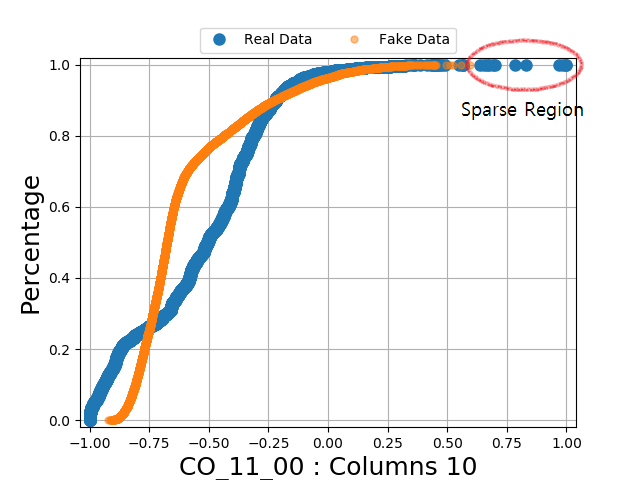
\includegraphics[trim={0 0.65cm 0 0},clip,width=0.26\textwidth]{images/CO_11_00___Columns_10.png}}
\subfigure[Ours,high-privacy,LACity]{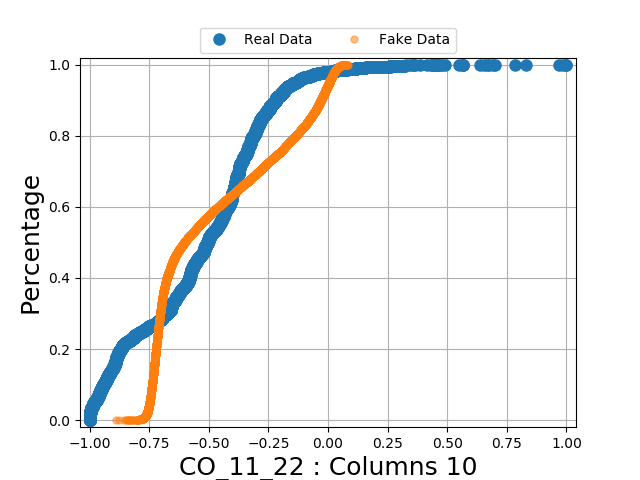
\includegraphics[trim={0 0.65cm 0 0},clip,width=0.26\textwidth]
{images/CO_11_22___Columns_10.png}}
\subfigure[DCGAN,LACity]{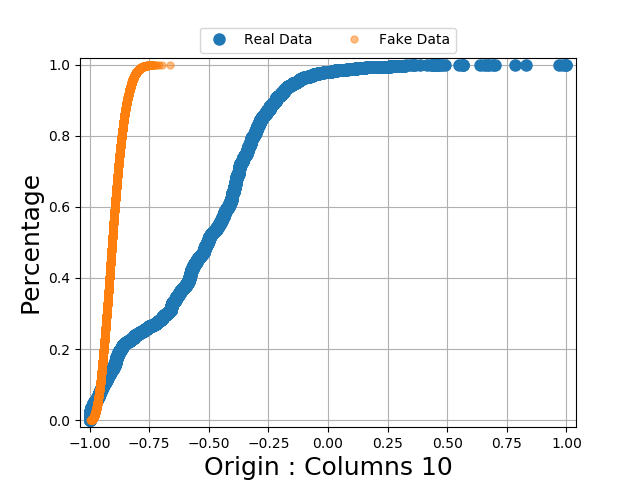
\includegraphics[trim={0 0.65cm 0 0},clip,width=0.26\textwidth]{images/Origin___Columns_10.png}} \\
% \subfigure[ARX1 (zero-privacy), LACity]{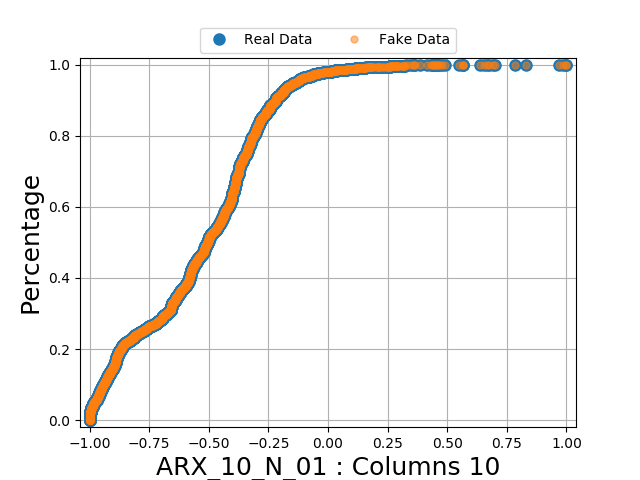
\includegraphics[trim={0 0.65cm 0 0},clip,width=0.24\textwidth]{LACity_ARX_10_N_01___Columns_10.png}}\\
\vspace{-1em}
\subfigure[Ours,low-privacy,Adult]{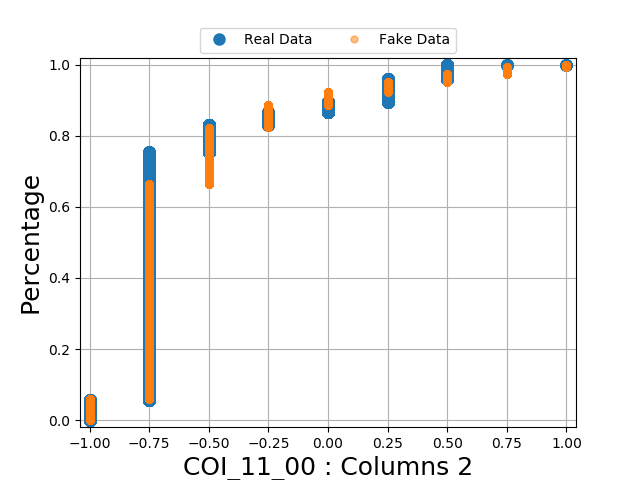
\includegraphics[trim={0 0.65cm 0 0},clip,width=0.26\textwidth]
{images/COI_11_00___Columns_2.png}}
\subfigure[Ours,high-privacy,Adult]{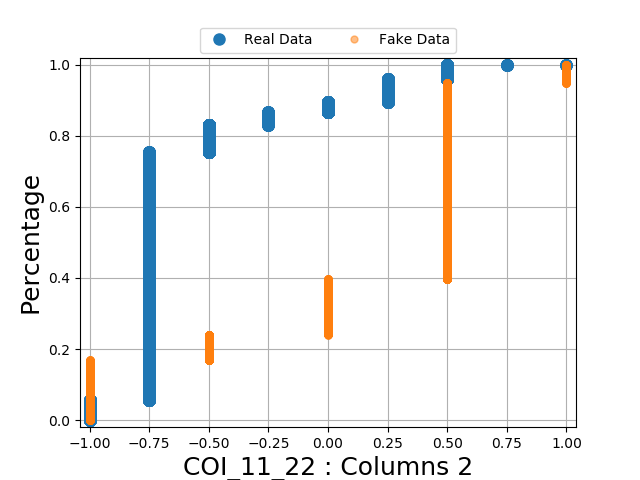
\includegraphics[trim={0 0.65cm 0 0},clip,width=0.26\textwidth]
{images/COI_11_22___Columns_2.png}}
\subfigure[DCGAN,Adult]{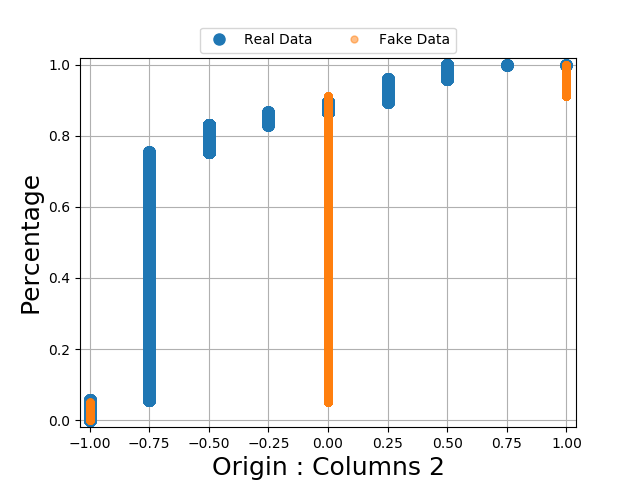
\includegraphics[trim={0 0.65cm 0 0},clip,width=0.26\textwidth]
{images/Origin___Columns_2.png}} \\
% \subfigure[sdcMicro, Adult]{\includegraphics[trim={0 0.65cm 0 0},clip,width=0.24\textwidth]
% {images/sdc_Adult___Columns_4.png}}\\
\vspace{-1em}
\subfigure[Ours,low-privacy,Health]{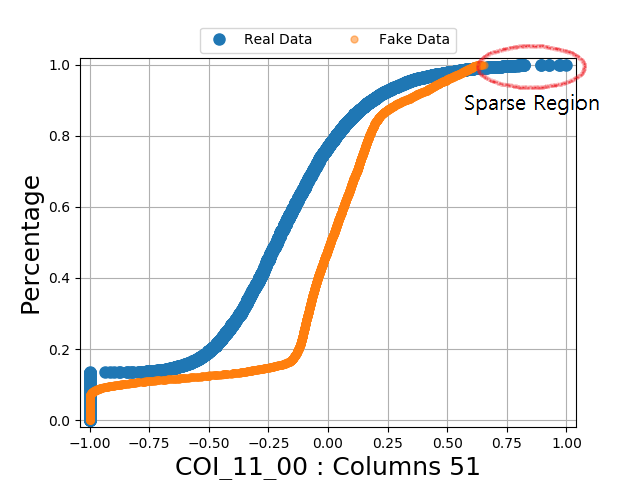
\includegraphics[trim={0 0.65cm 0 0},clip,width=0.26\textwidth]
{images/COI_11_00___Columns_51.png}}
\subfigure[Ours,high-privacy,Health]{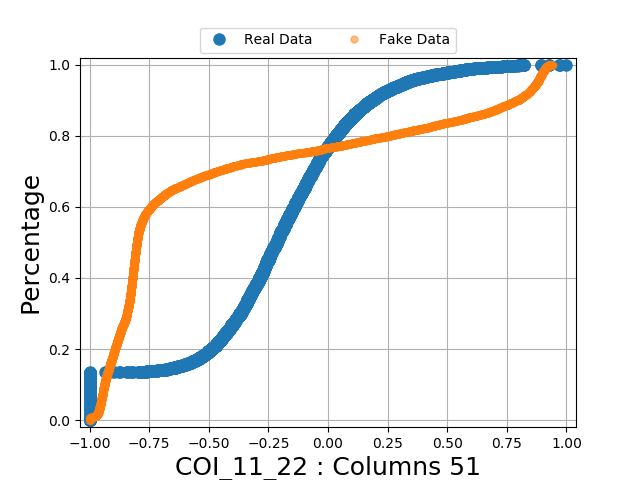
\includegraphics[trim={0 0.65cm 0 0},clip,width=0.26\textwidth]
{images/COI_11_22___Columns_51.png}}
\subfigure[DCGAN,Health]{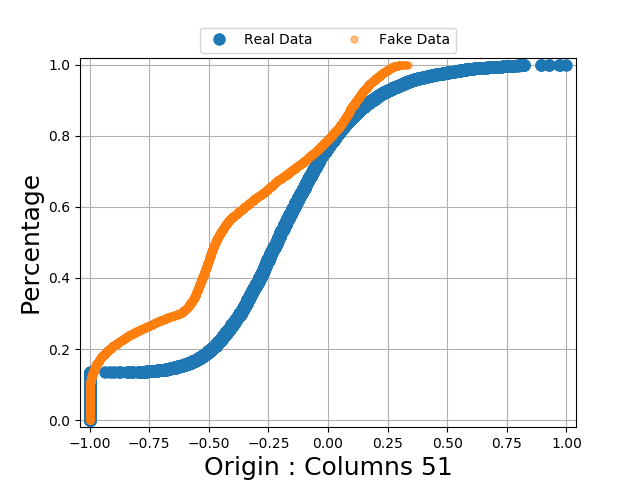
\includegraphics[trim={0 0.65cm 0 0},clip,width=0.26\textwidth]
{images/Origin___Columns_51.png}}\\
\vspace{-1em}
\subfigure[Ours,low-privacy,LACity]{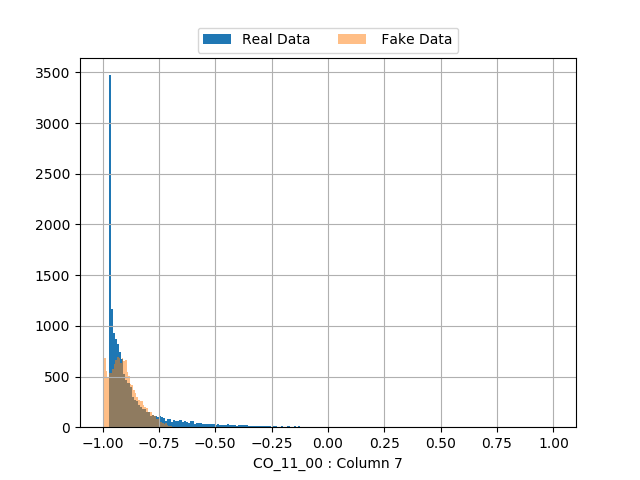
\includegraphics[trim={0 0.65cm 0 0},clip,width=0.26\textwidth]
{images/CO_11_00___Column_7.png}}
\subfigure[Ours,high-privacy,LACity]{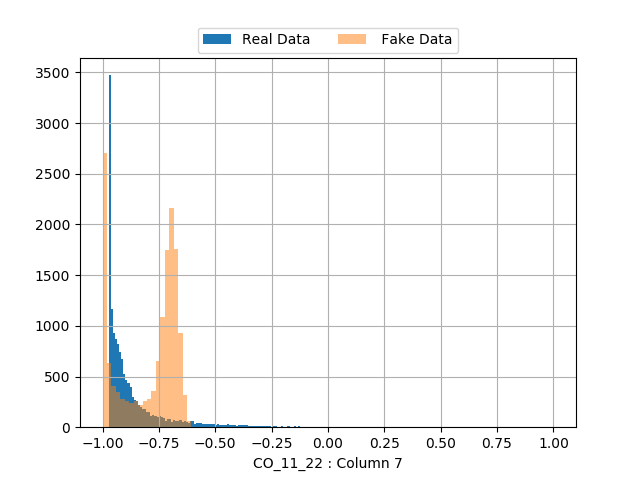
\includegraphics[trim={0 0.65cm 0 0},clip,width=0.26\textwidth]
{images/CO_11_22___Column_7.png}}
\subfigure[DCGAN,LACity]{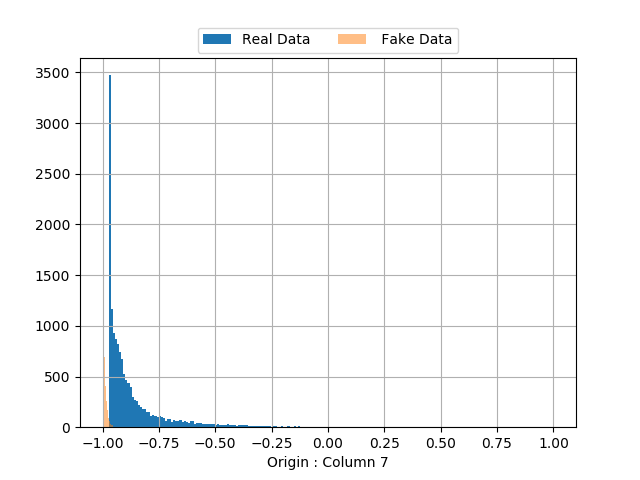
\includegraphics[trim={0 0.65cm 0 0},clip,width=0.26\textwidth]
{images/Origin___Column_7.png}}\\
\vspace{-1em}
\subfigure[Ours,low-privacy,Airline]{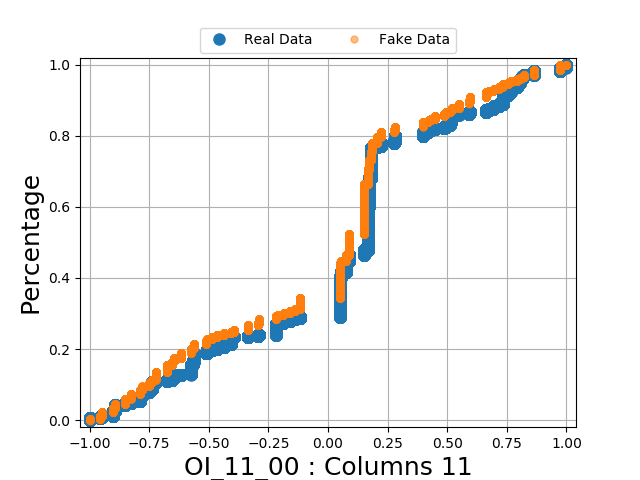
\includegraphics[trim={0 0.65cm 0 0},clip,width=0.26\textwidth]
{images/tgan_low_OI_11_00___Columns_11.png}}
\subfigure[Ours,high-privacy,Airline]{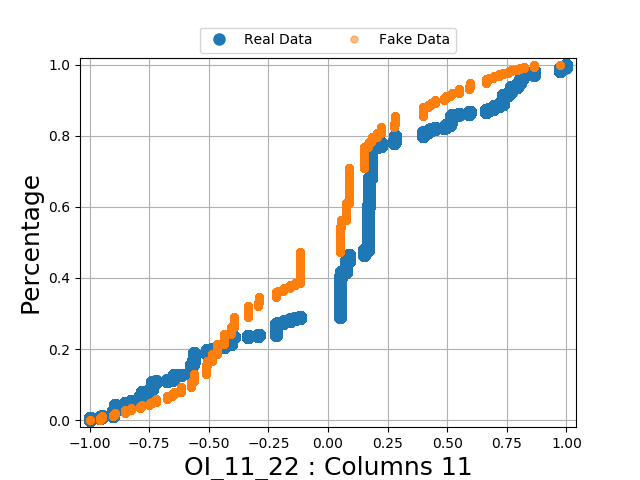
\includegraphics[trim={0 0.65cm 0 0},clip,width=0.26\textwidth]
{images/tgan_high_OI_11_22___Columns_11.png}}
\subfigure[DCGAN,Airline]{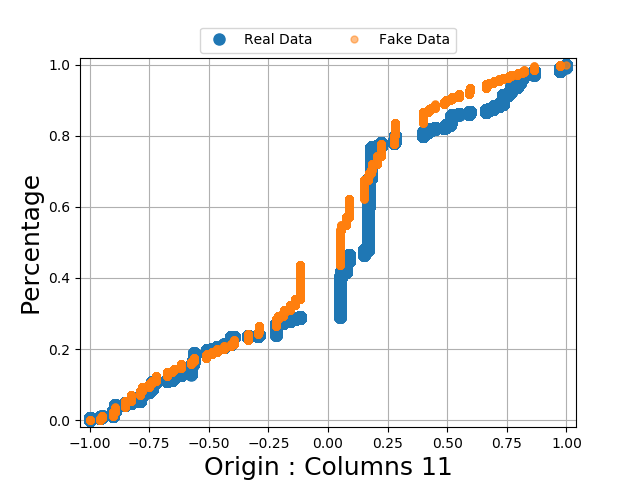
\includegraphics[trim={0 0.65cm 0 0},clip,width=0.26\textwidth]
{images/dcgan_Origin___Columns_11.png}}\\
\vspace{-1em}
\caption{Cumulative distributions and histograms of sensitive attributes by DCGAN and table-GAN. X-axes are normalized. Statistics of the original attributes are marked in blue, and synthetic ones are marked in orange.}\label{fig:cd}
\end{figure*}

\subsubsection{Computing Environments}
We implemented the proposed table-GAN based on Tensorflow and trained in a server with an i7 3.4 Ghz CPU and GTX970 GPU. We did not use any expensive components for the experiments. Even in the entry-level server, it took at most 20 minutes to generate synthetic tables, as shown in Table~\ref{T:time}.

\begin{figure*}[t]
\centering
\subfigure[Ours,low-privacy,LACity]{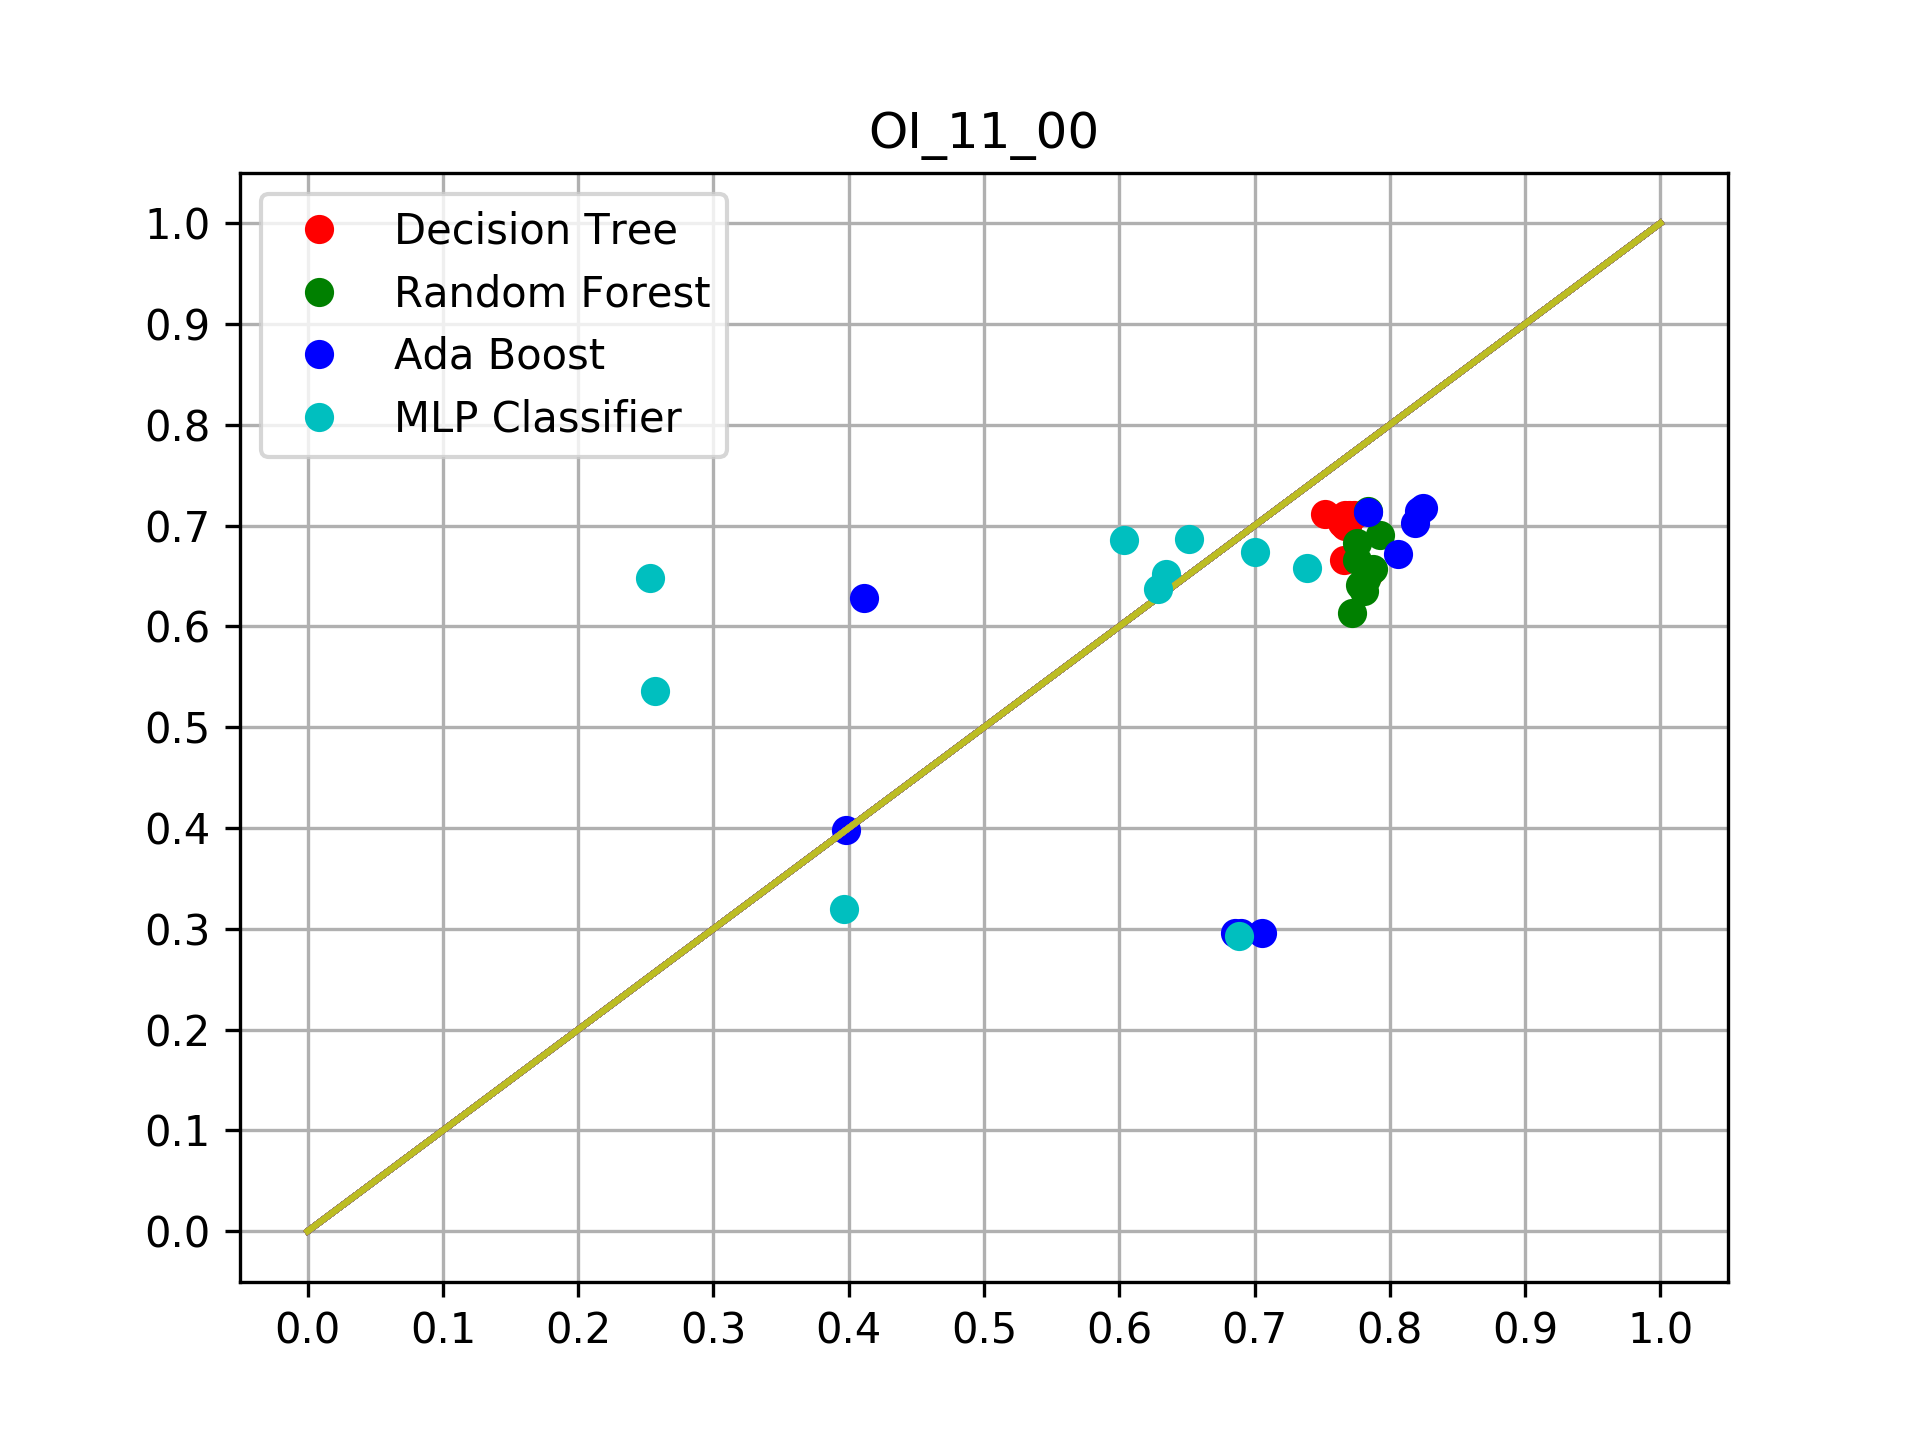
\includegraphics[trim={1cm 0.8cm 1cm 1.37cm},clip,width=0.24\textwidth]{images/12.png}}
\subfigure[Ours,high-privacy,LACity]{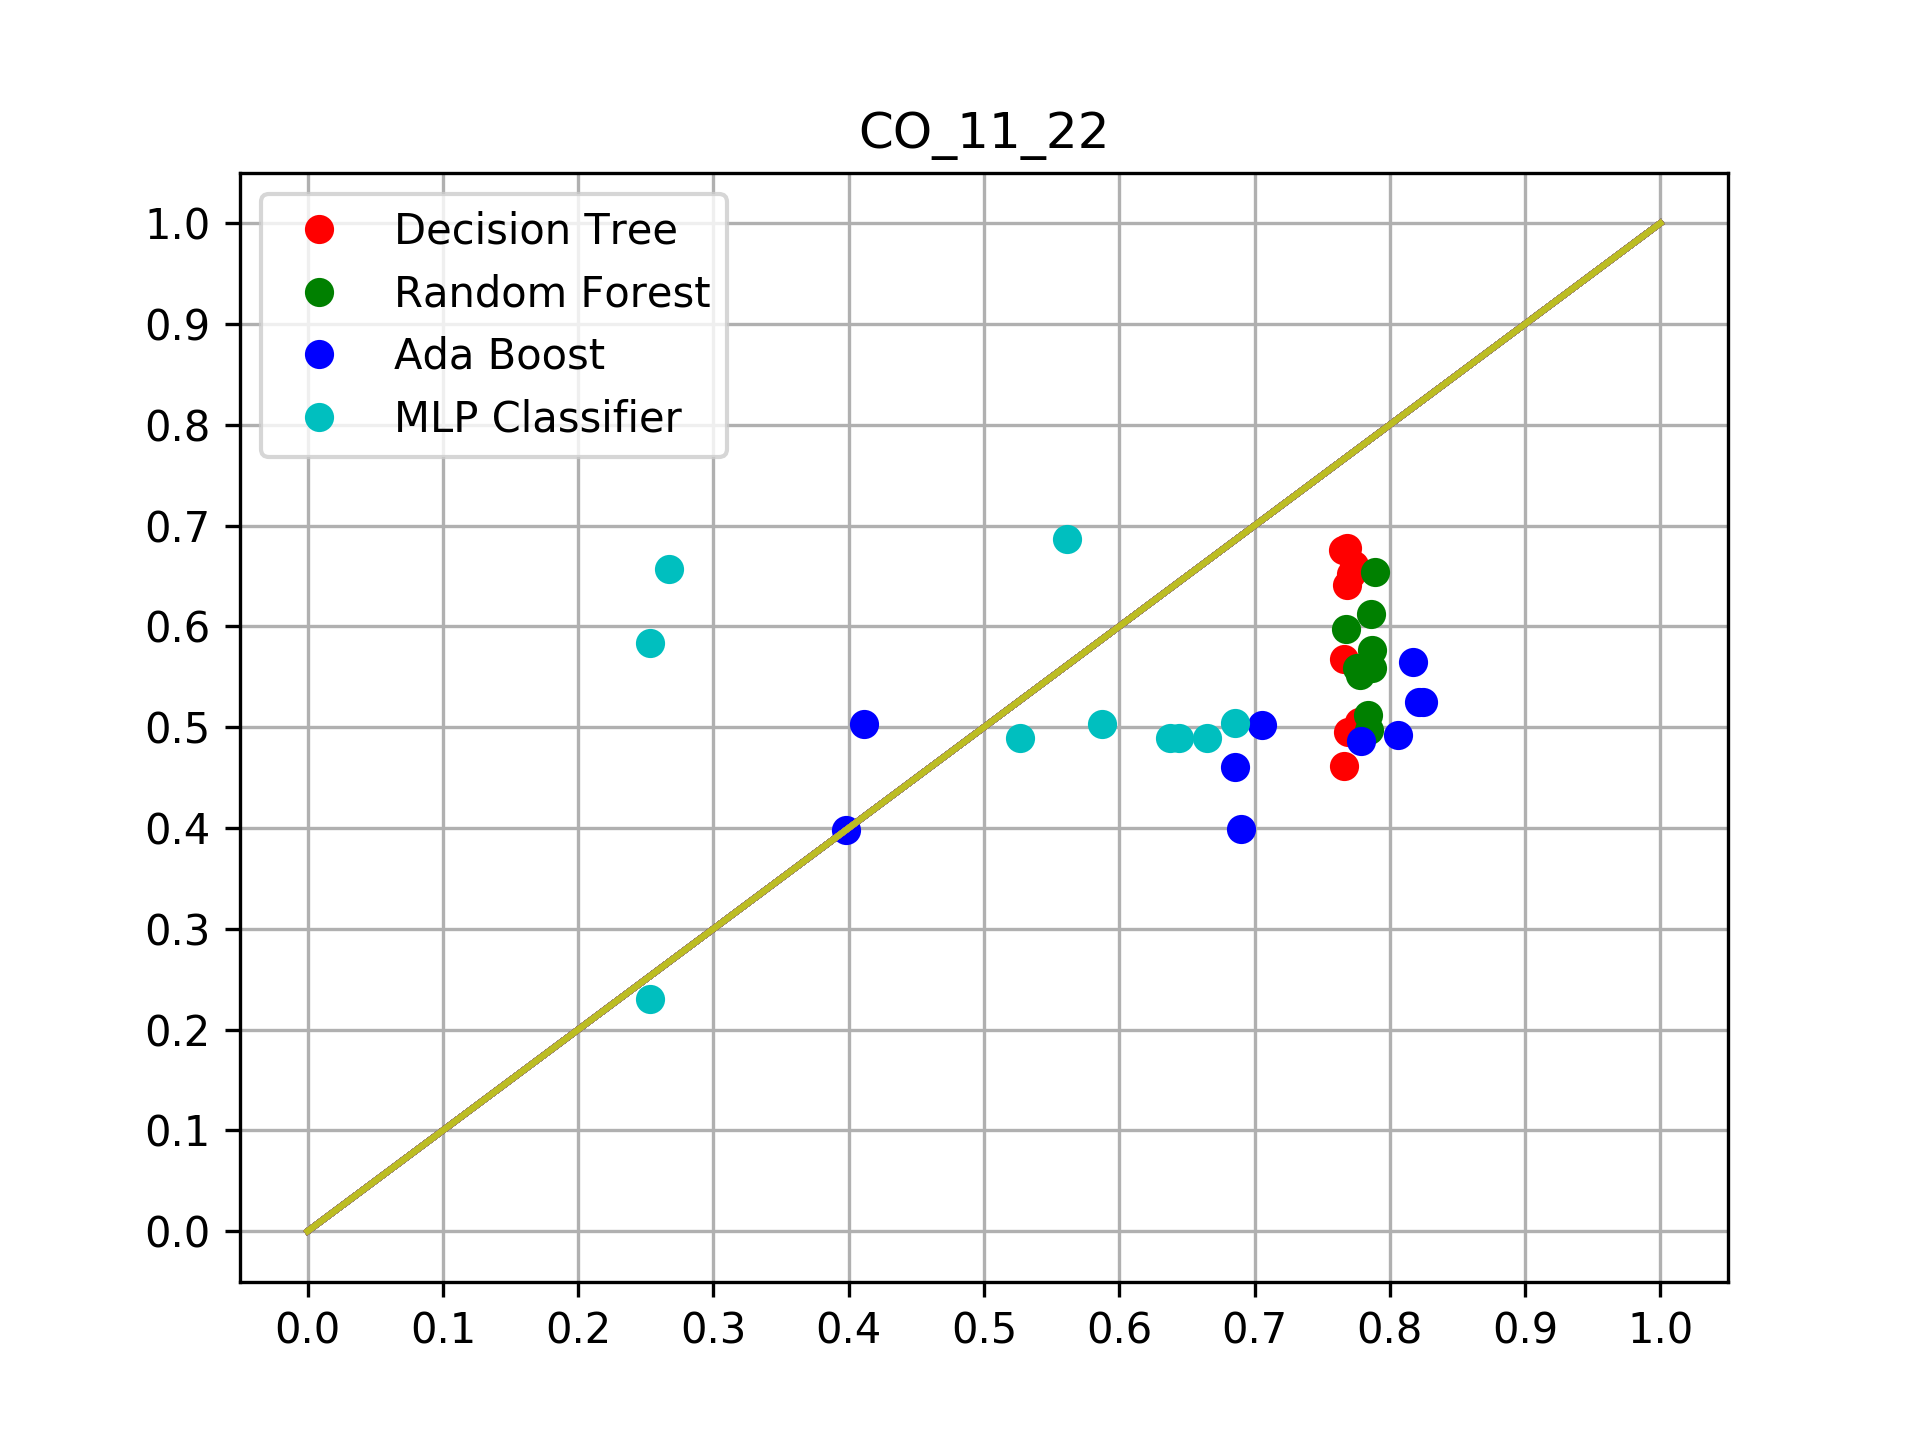
\includegraphics[trim={1cm 0.8cm 1cm 1.37cm},clip,width=0.24\textwidth]
{images/10.png}}
\subfigure[The best of ARX,LACity]{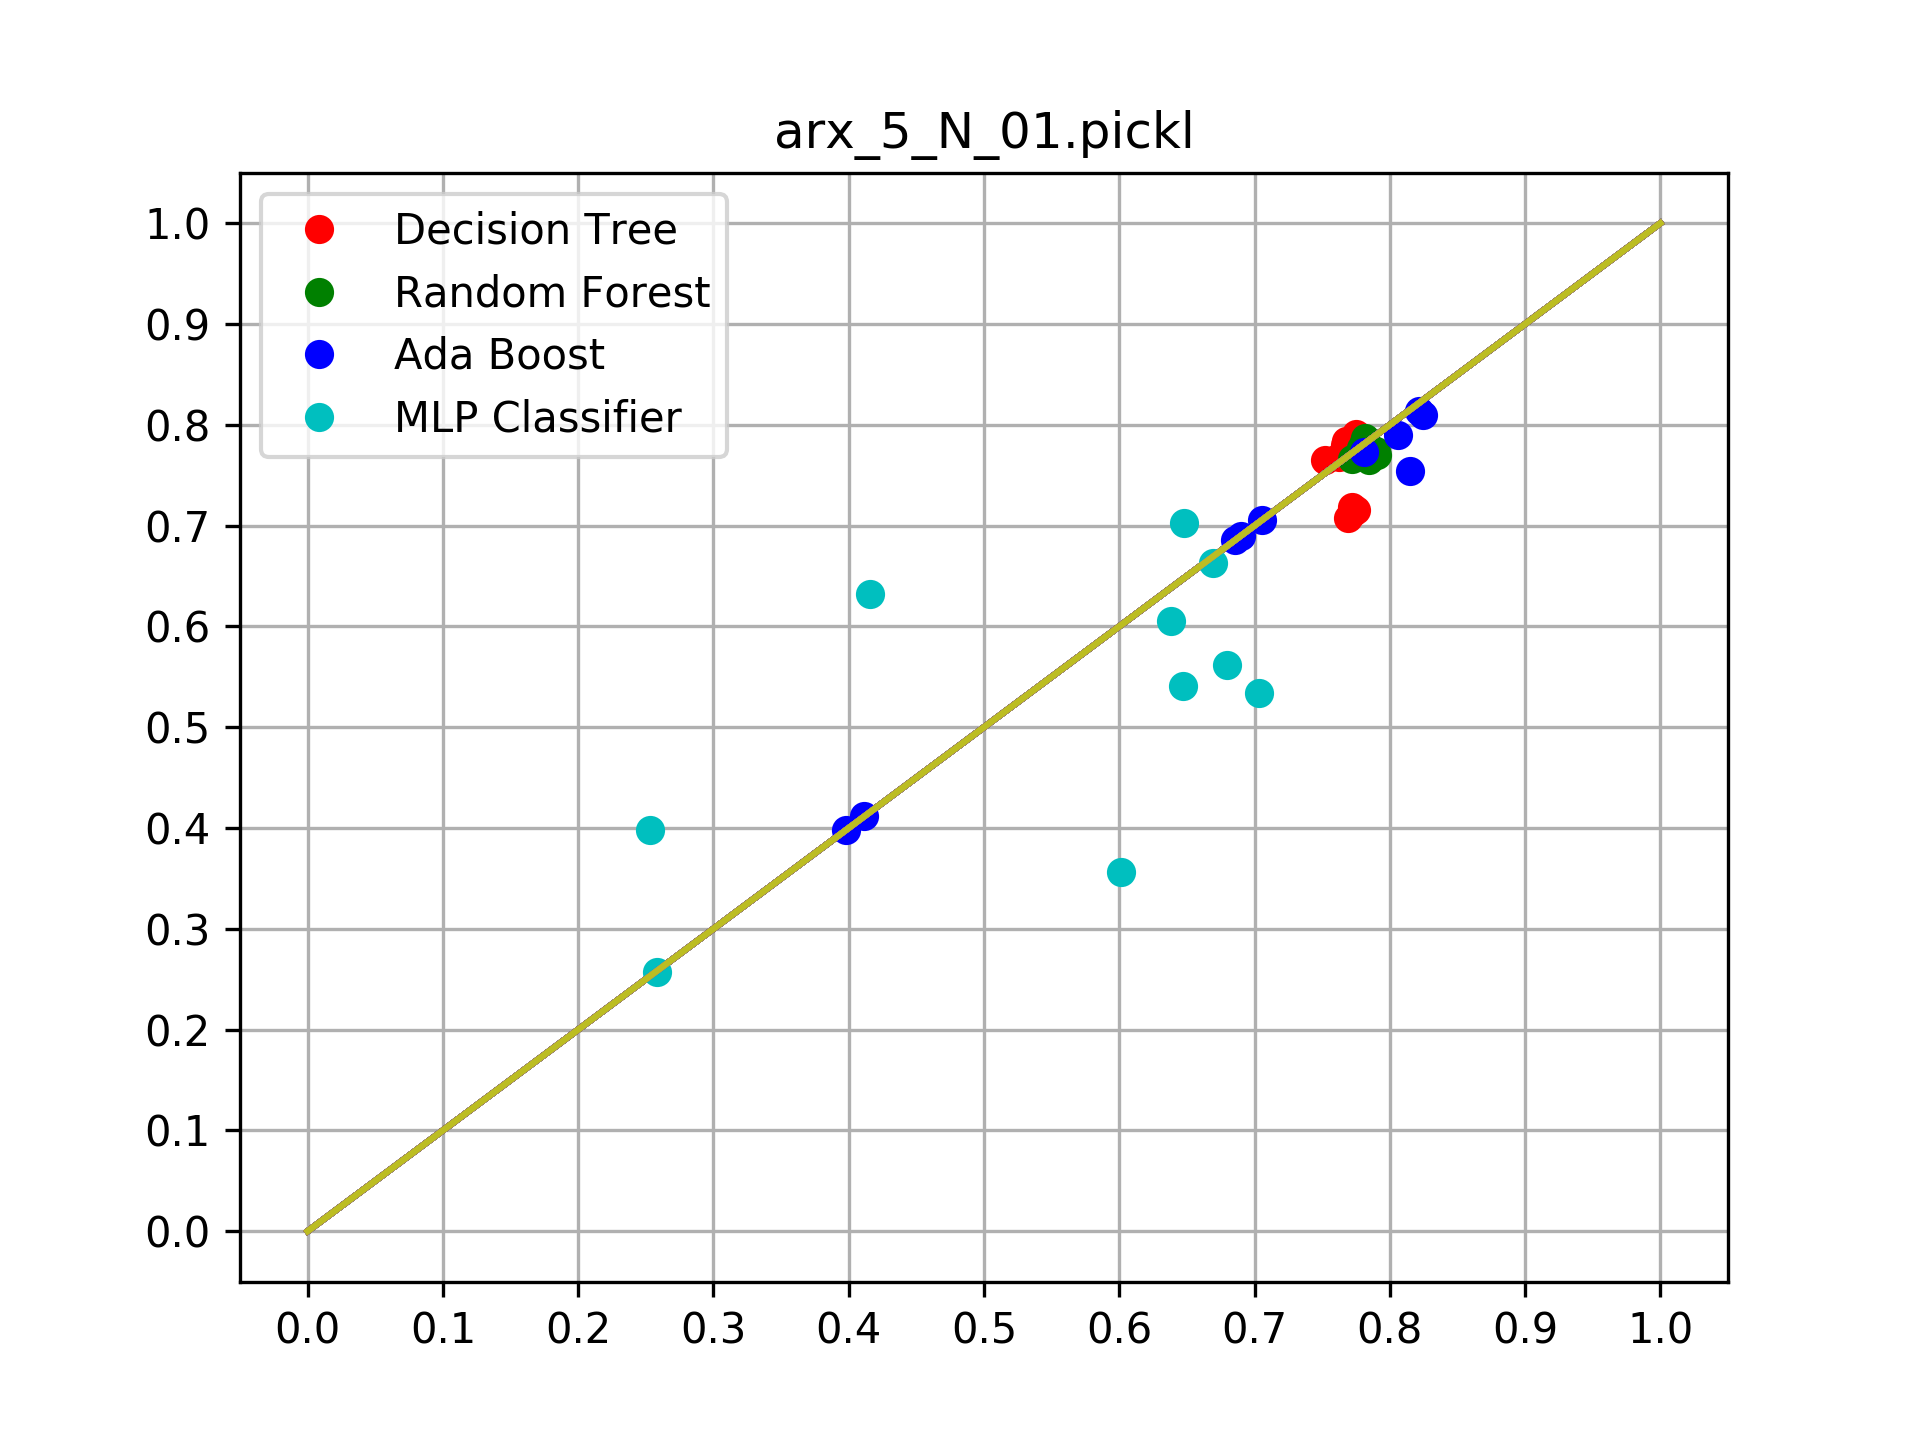
\includegraphics[trim={1cm 0.8cm 1cm 1.37cm},clip,width=0.24\textwidth]{images/23.png}}
\subfigure[The best of sdcMicro,LACity]{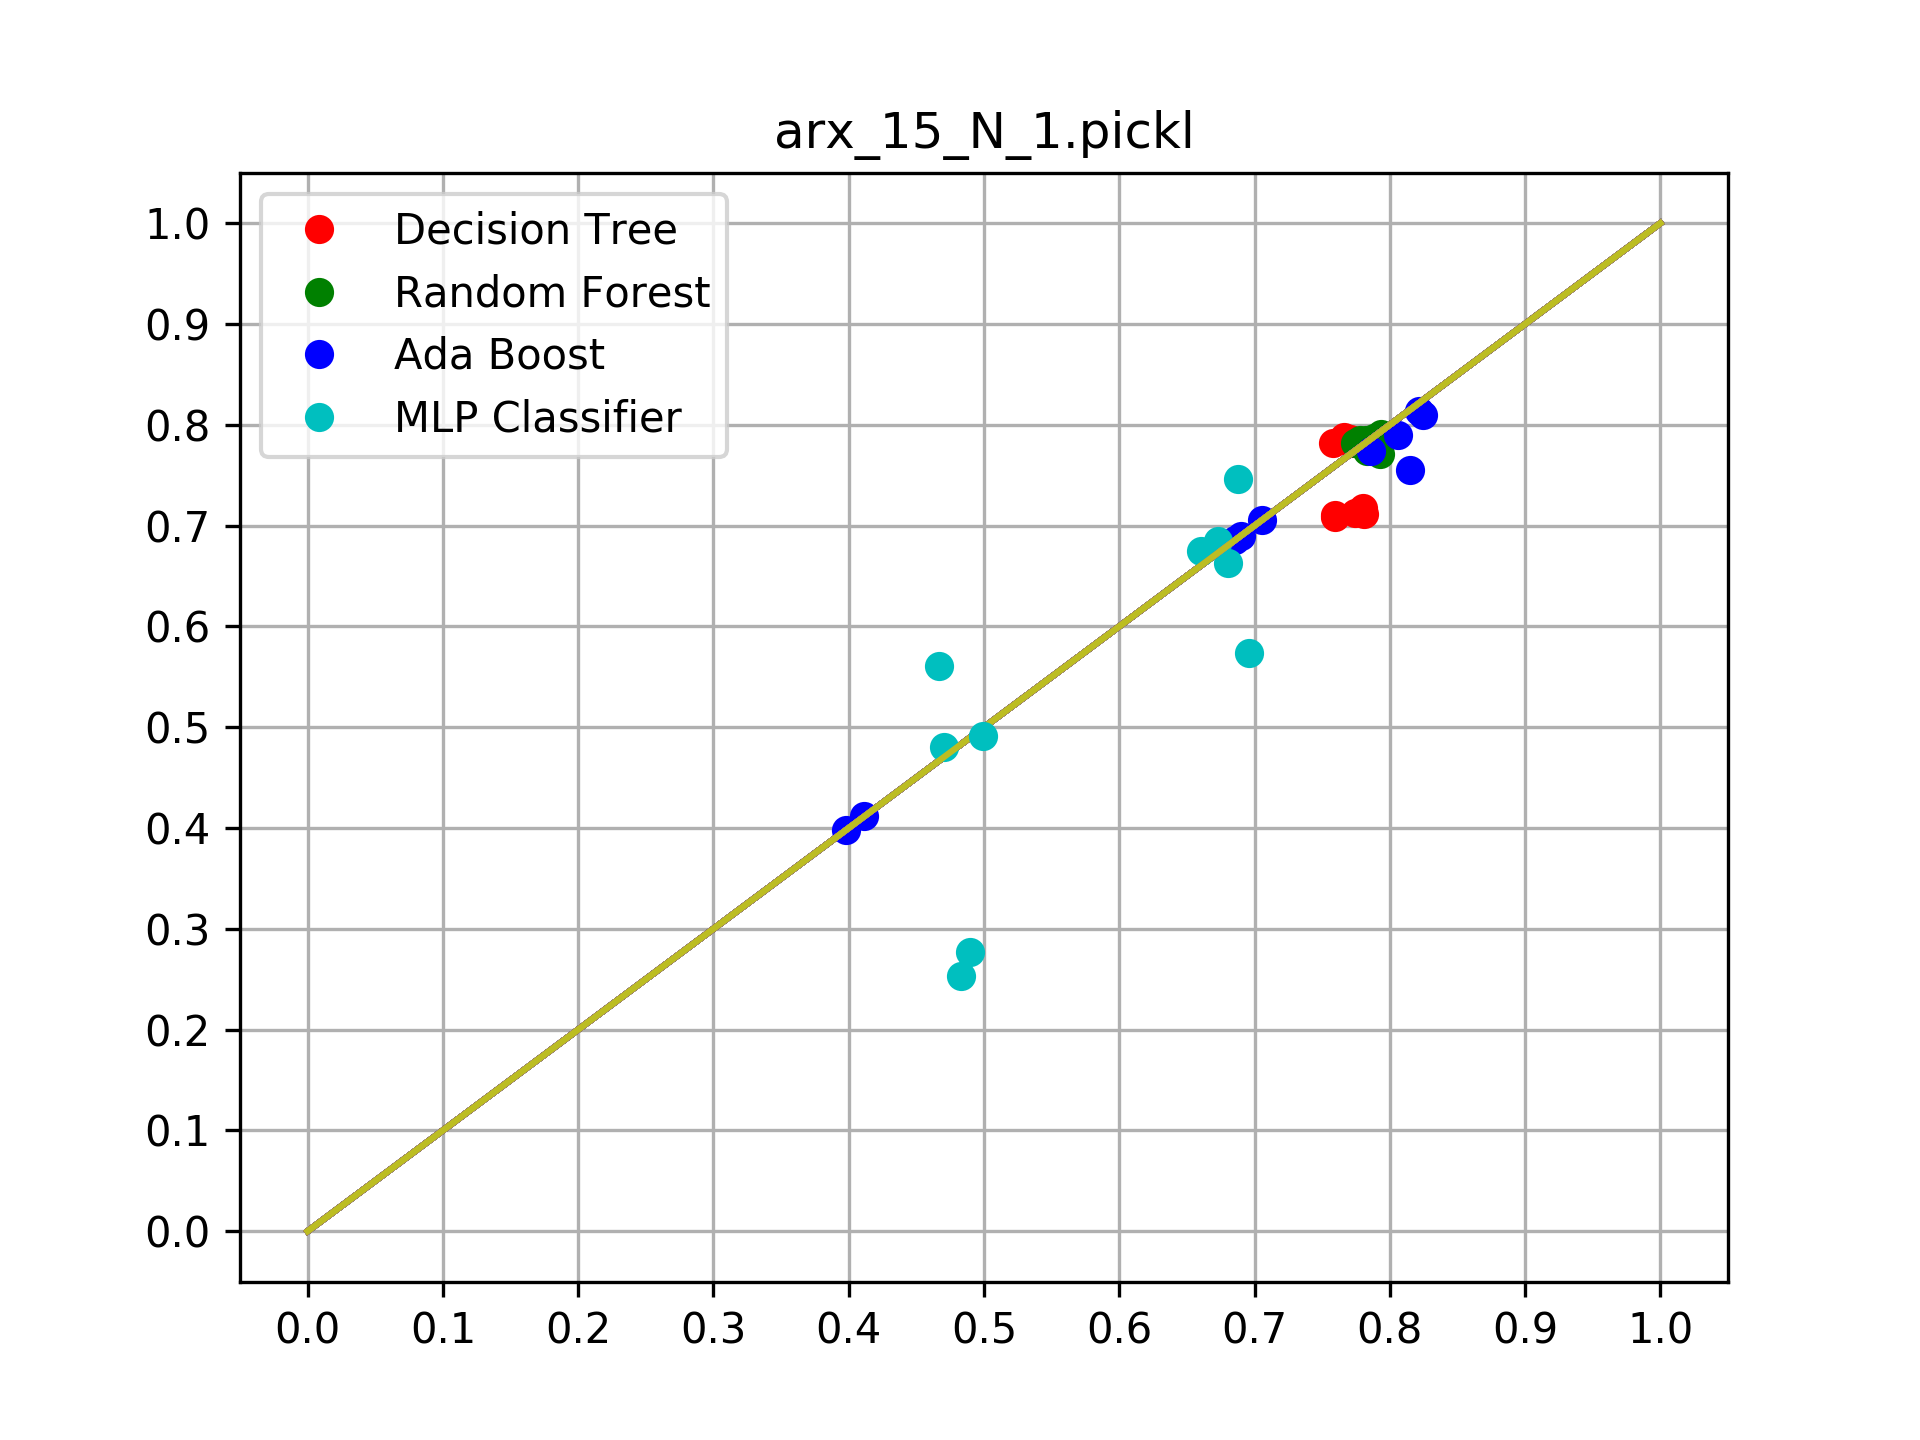
\includegraphics[trim={1cm 0.8cm 1cm 1.37cm},clip,width=0.24\textwidth]{images/25.png}}\\
\vspace{-1em}
\subfigure[Ours,low-privacy,Adult]{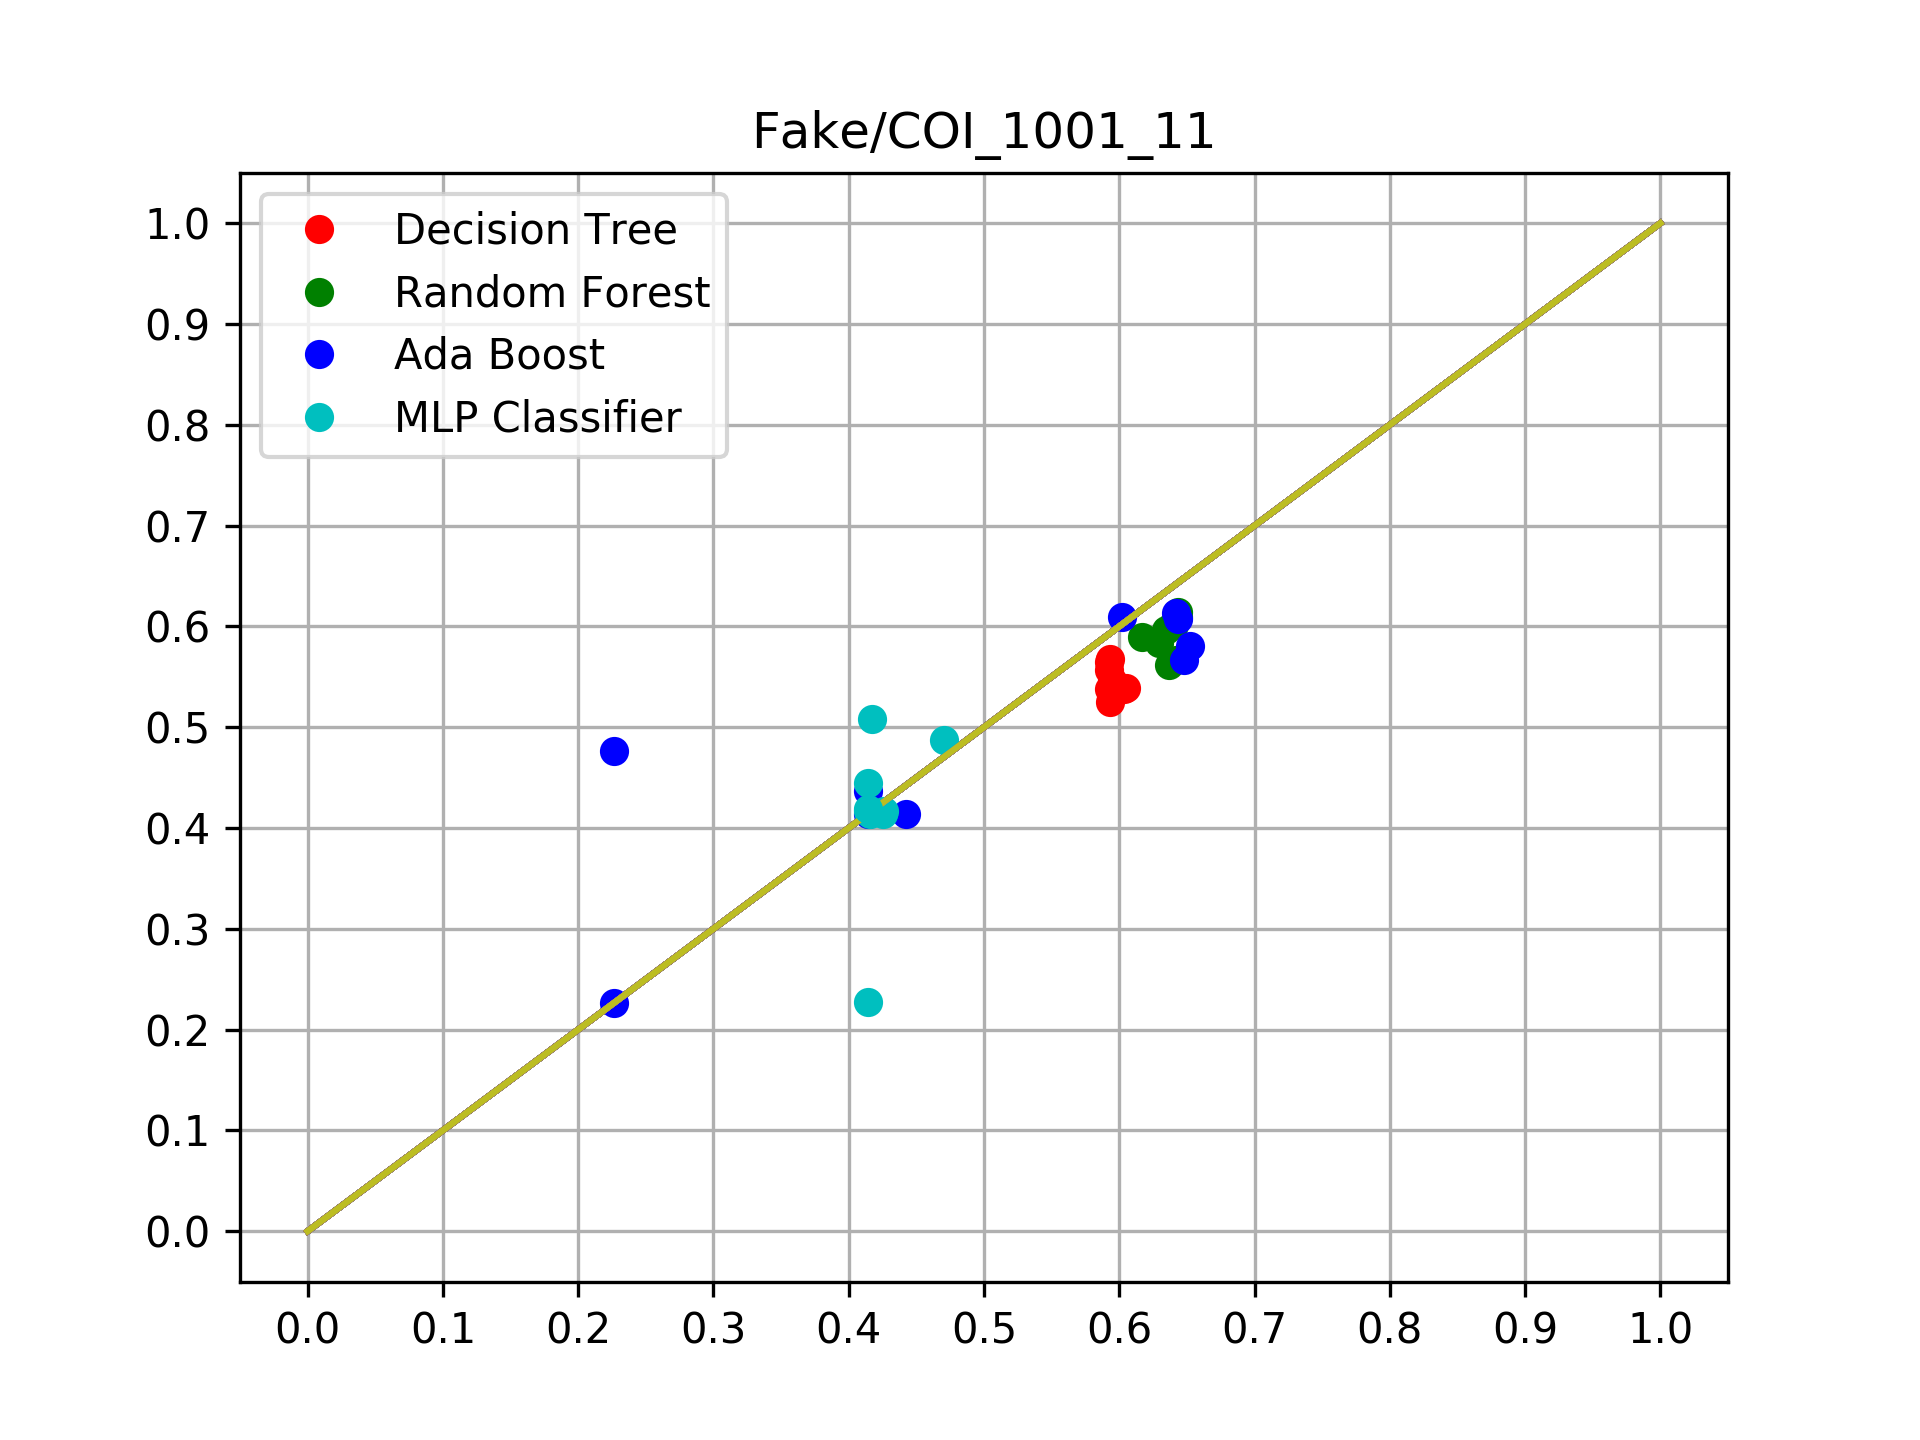
\includegraphics[trim={1cm 0.8cm 1cm 1.37cm},clip,width=0.24\textwidth]{images/Adult_16.png}}
\subfigure[Ours,high-privacy,Adult]{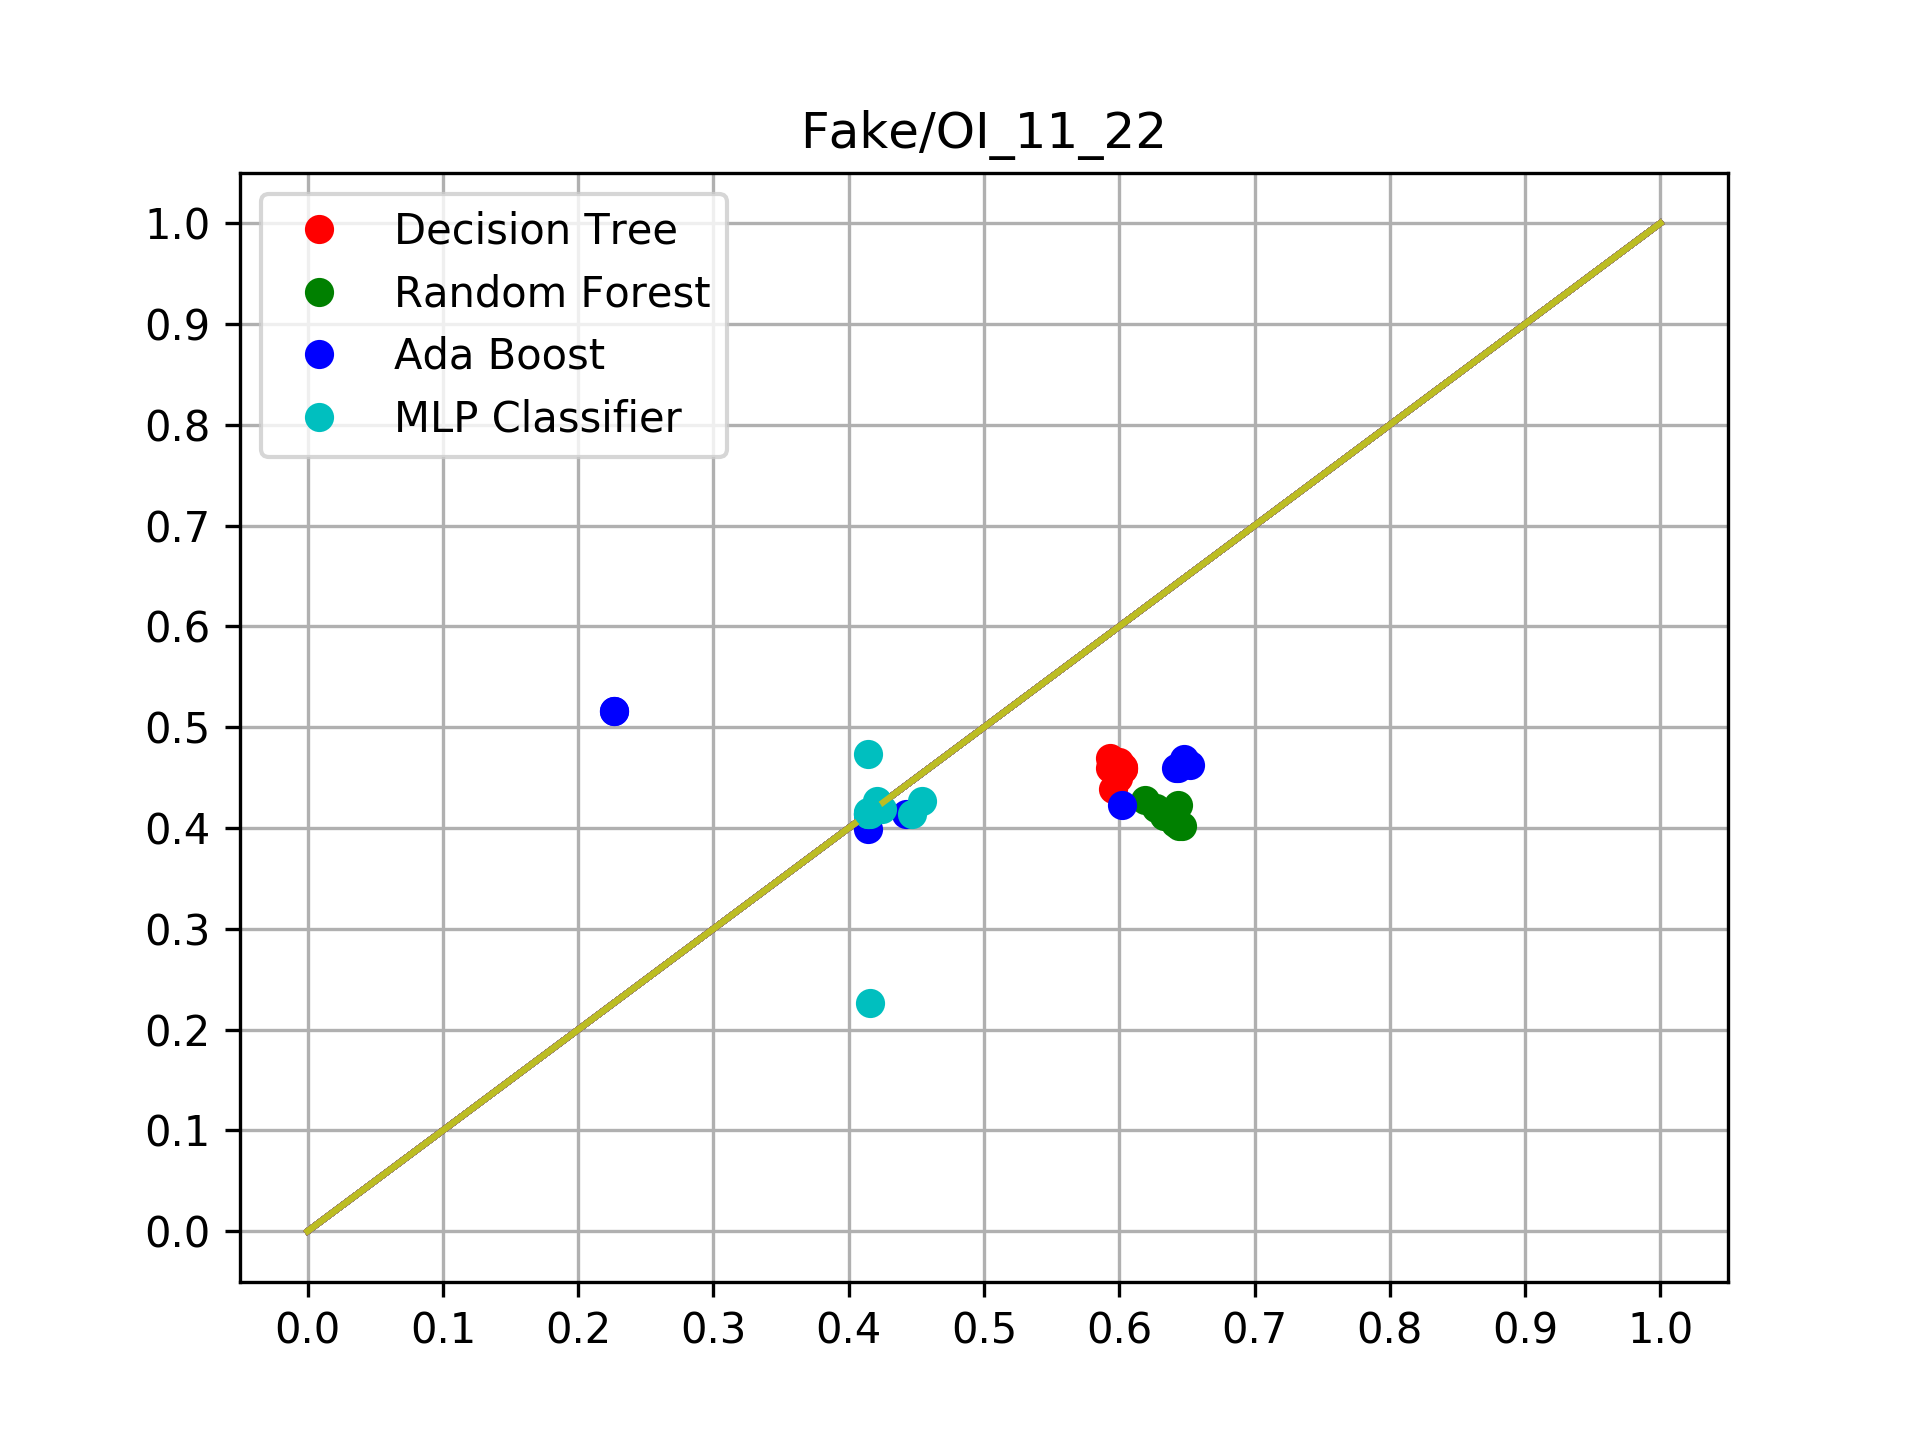
\includegraphics[trim={1cm 0.8cm 1cm 1.37cm},clip,width=0.24\textwidth]
{images/Adult_4.png}}
\subfigure[The best of ARX,Adult]{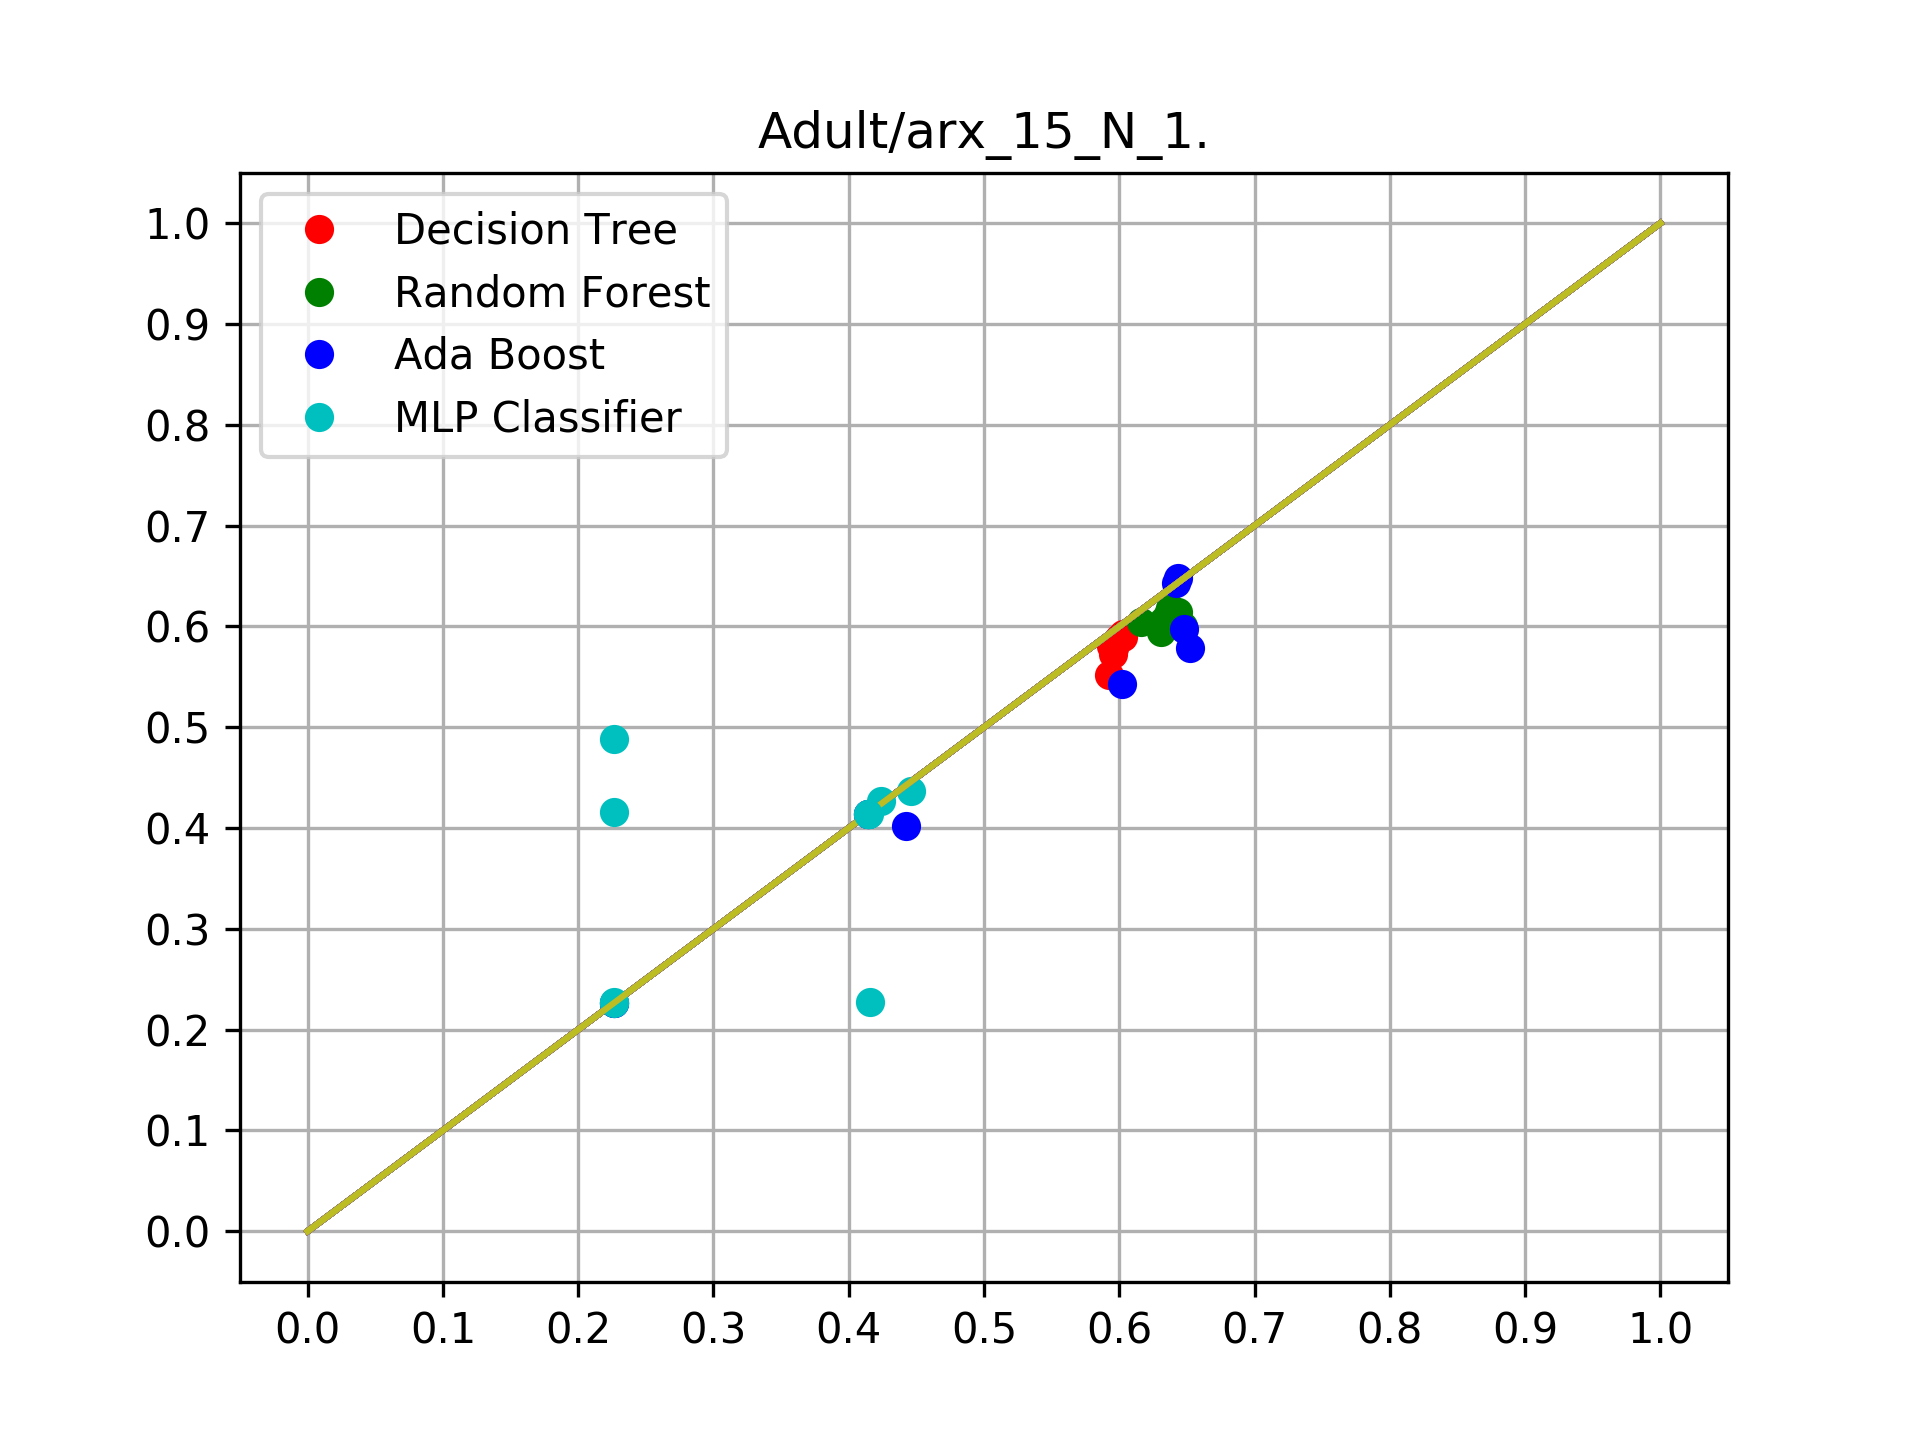
\includegraphics[trim={1cm 0.8cm 1cm 1.37cm},clip,width=0.24\textwidth]{images/ARX_Adult_6.png}}
\subfigure[The best of sdcMicro,Adult]{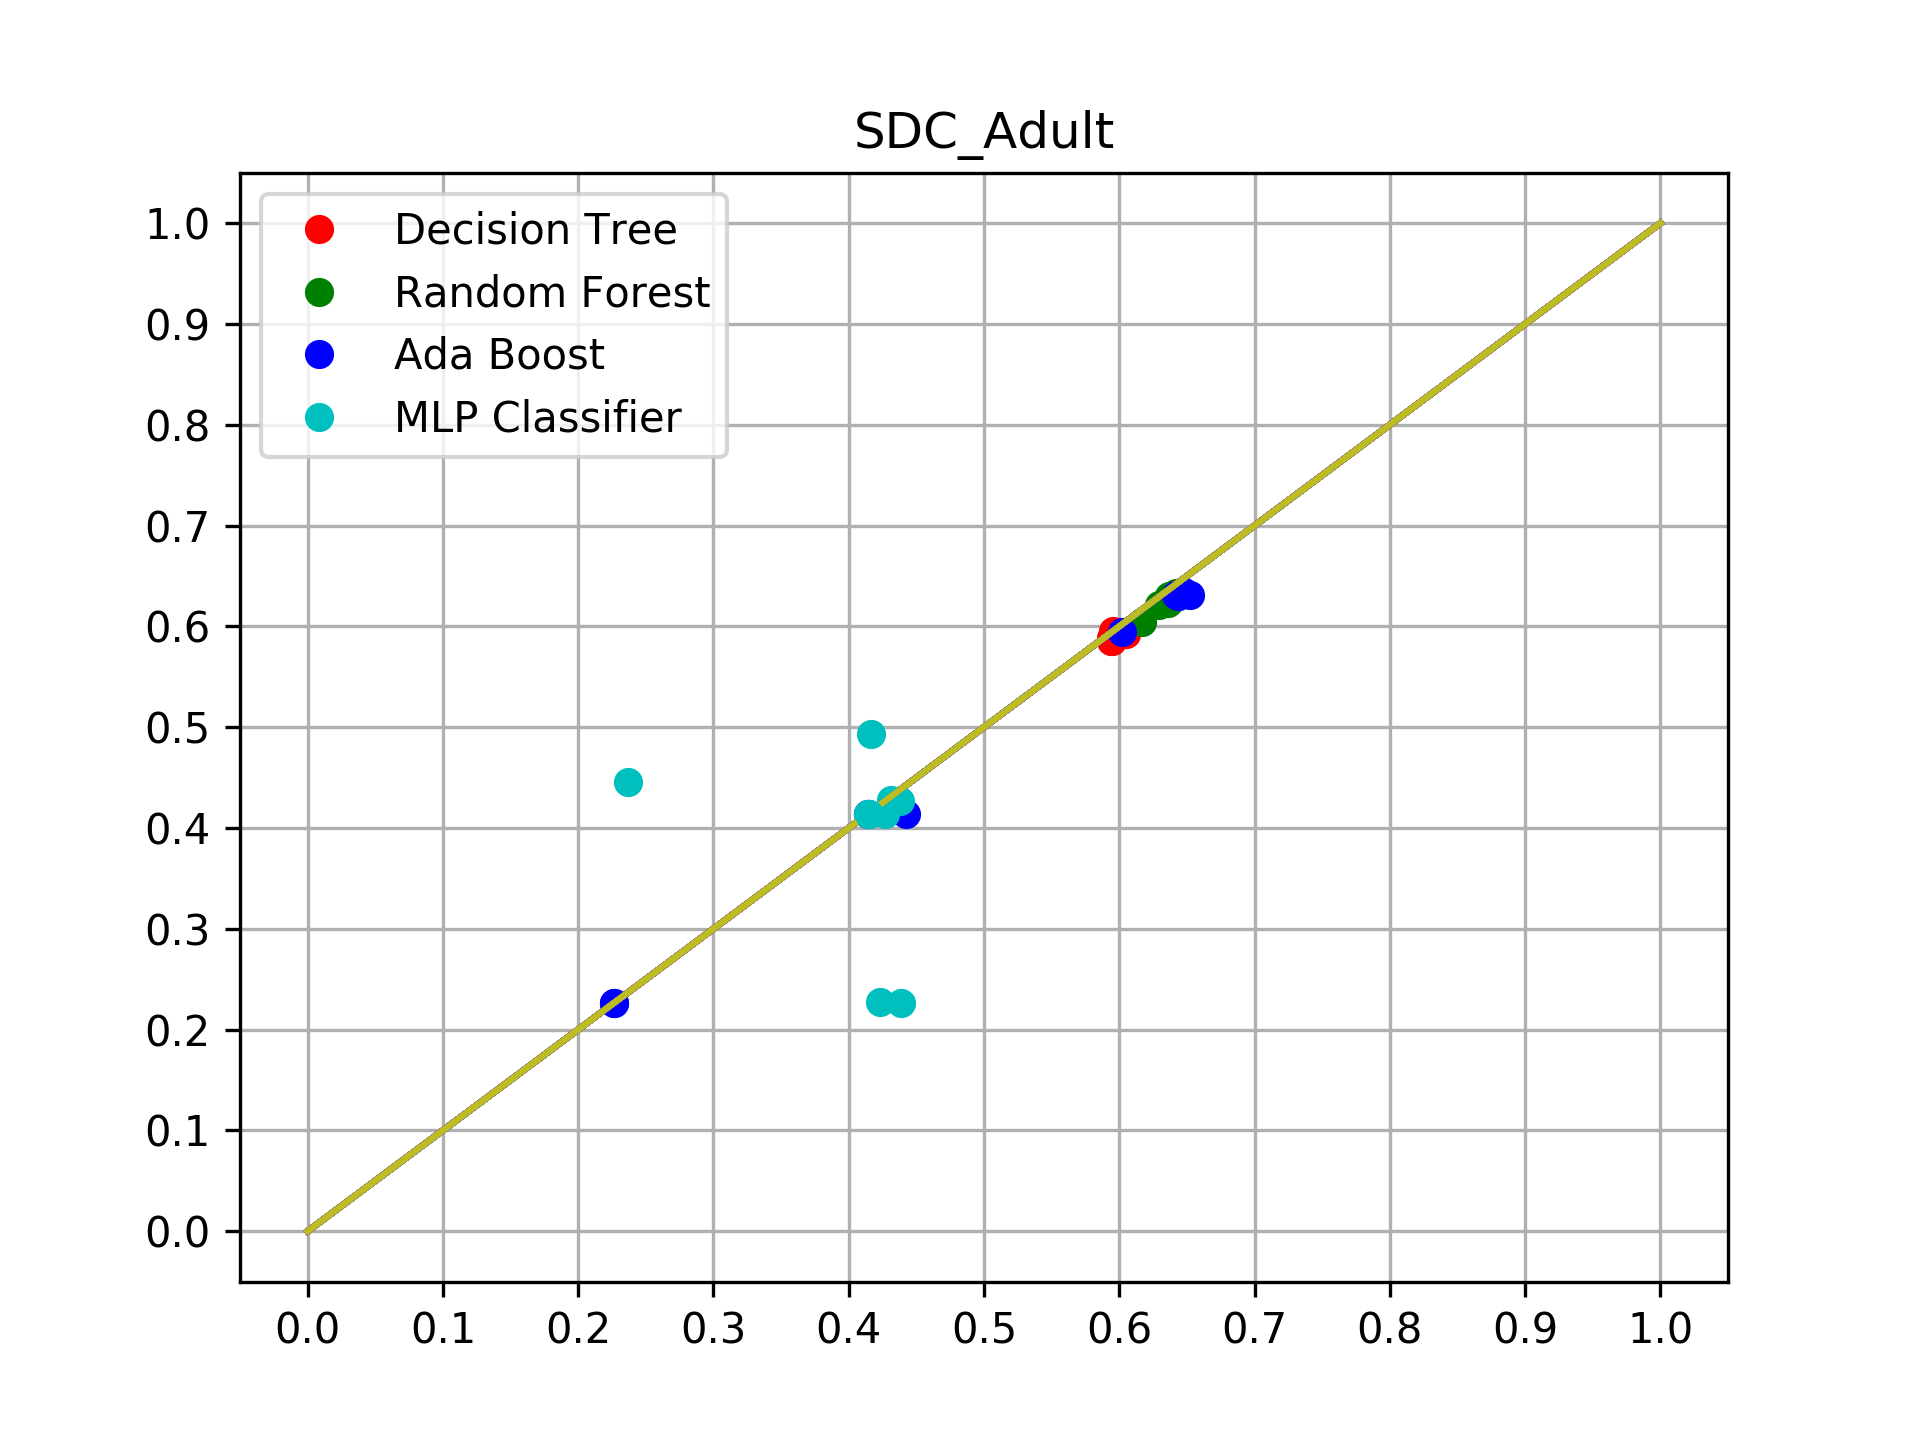
\includegraphics[trim={1cm 0.8cm 1cm 1.37cm},clip,width=0.24\textwidth]{images/SDC_Adult_1.png}}\\
\vspace{-1em}
\subfigure[Ours,low-privacy,Health]{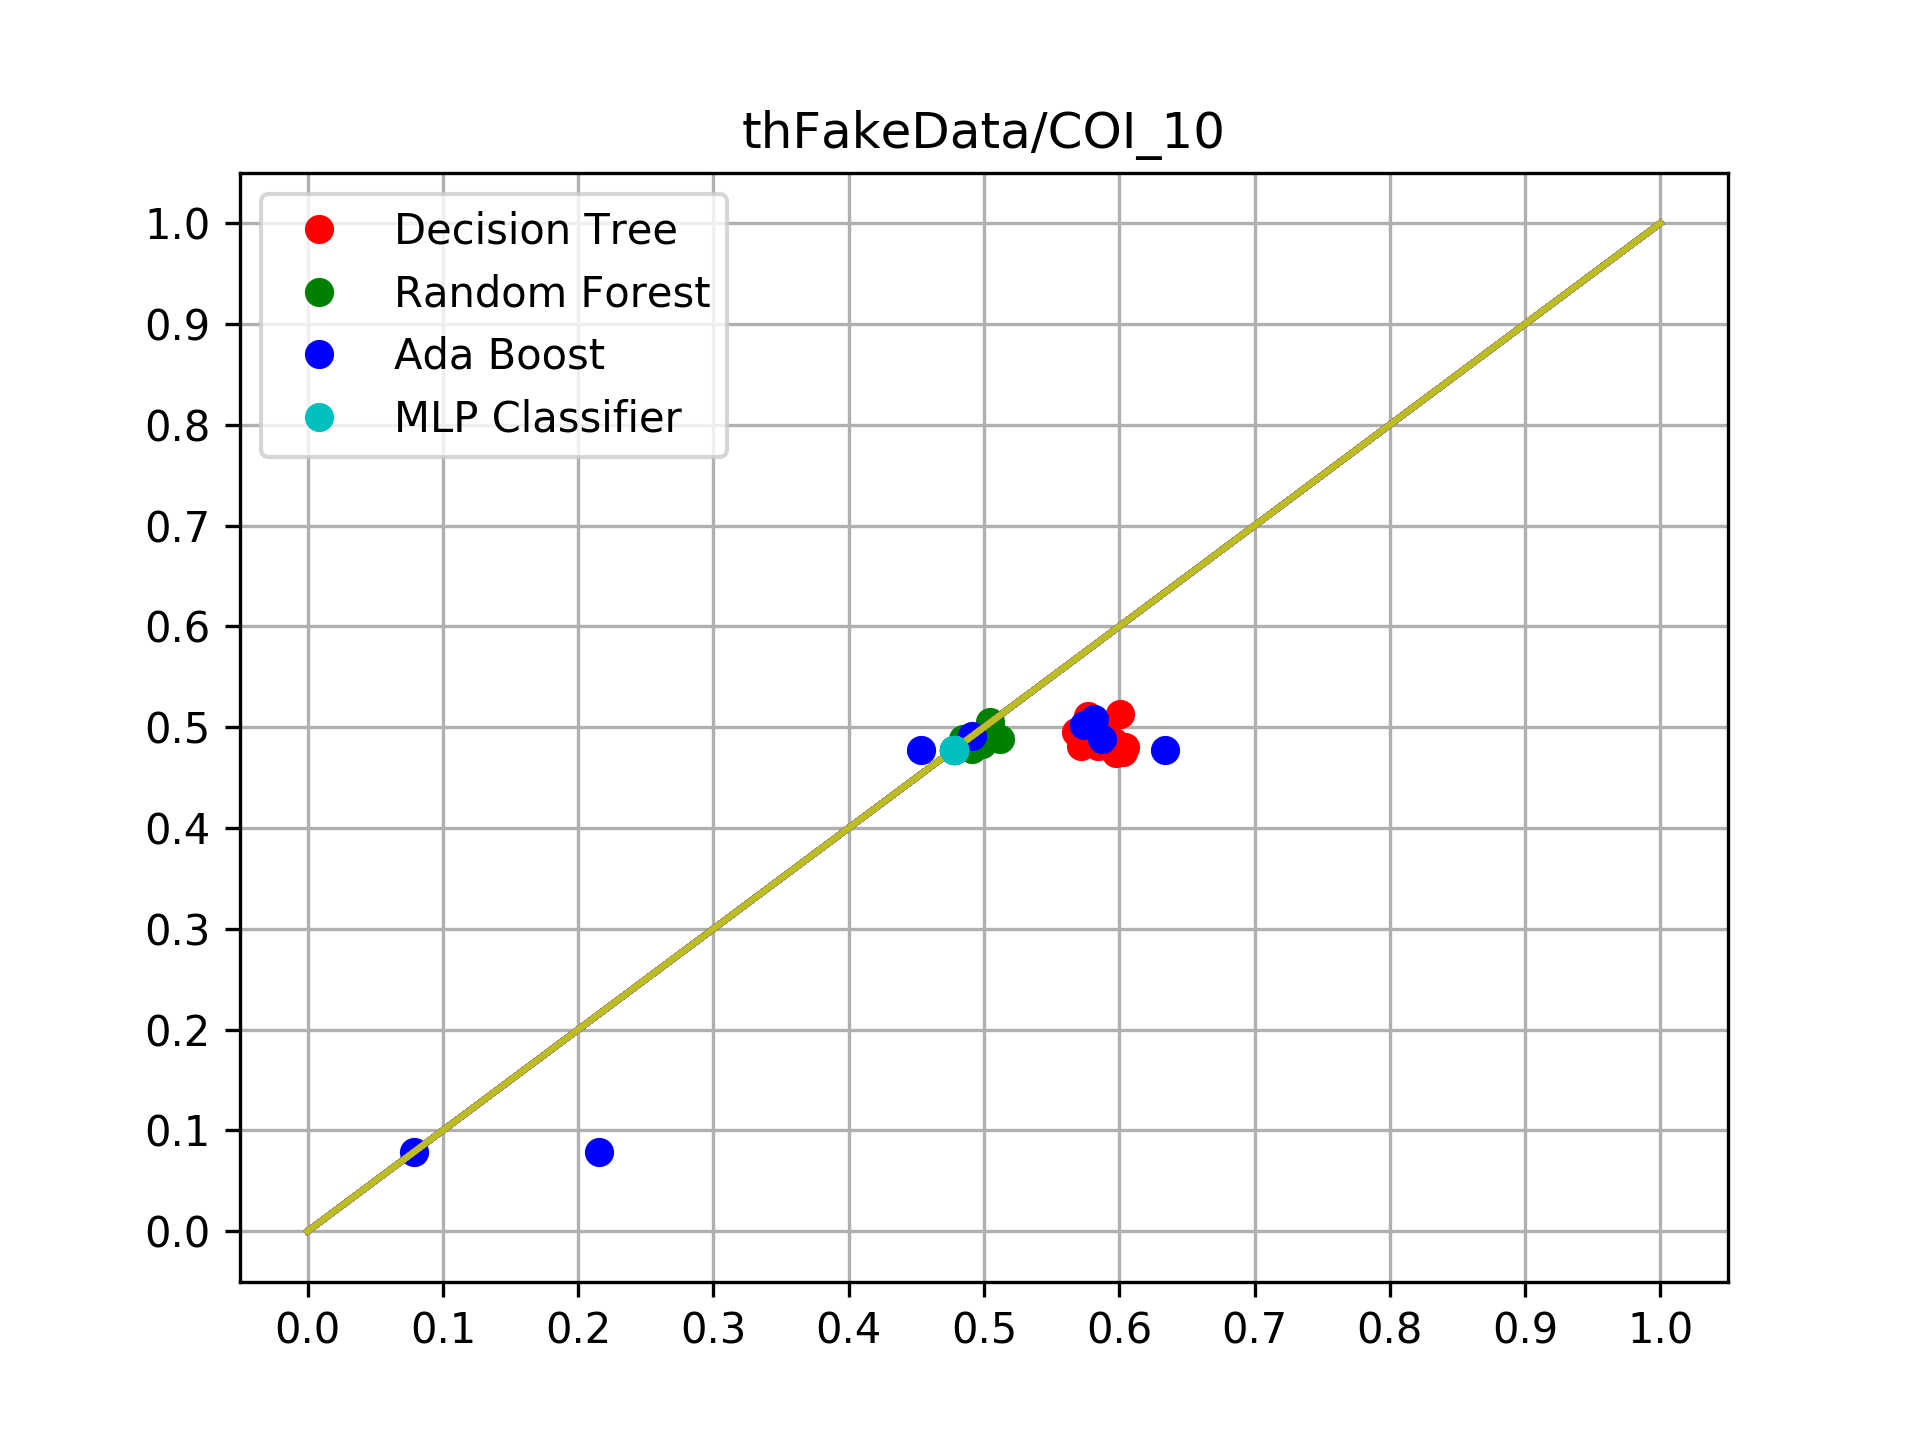
\includegraphics[trim={1cm 0.8cm 1cm 1.37cm},clip,width=0.24\textwidth]
{images/Health_DCGAN_14.png}}
\subfigure[Ours,high-privacy,Health]{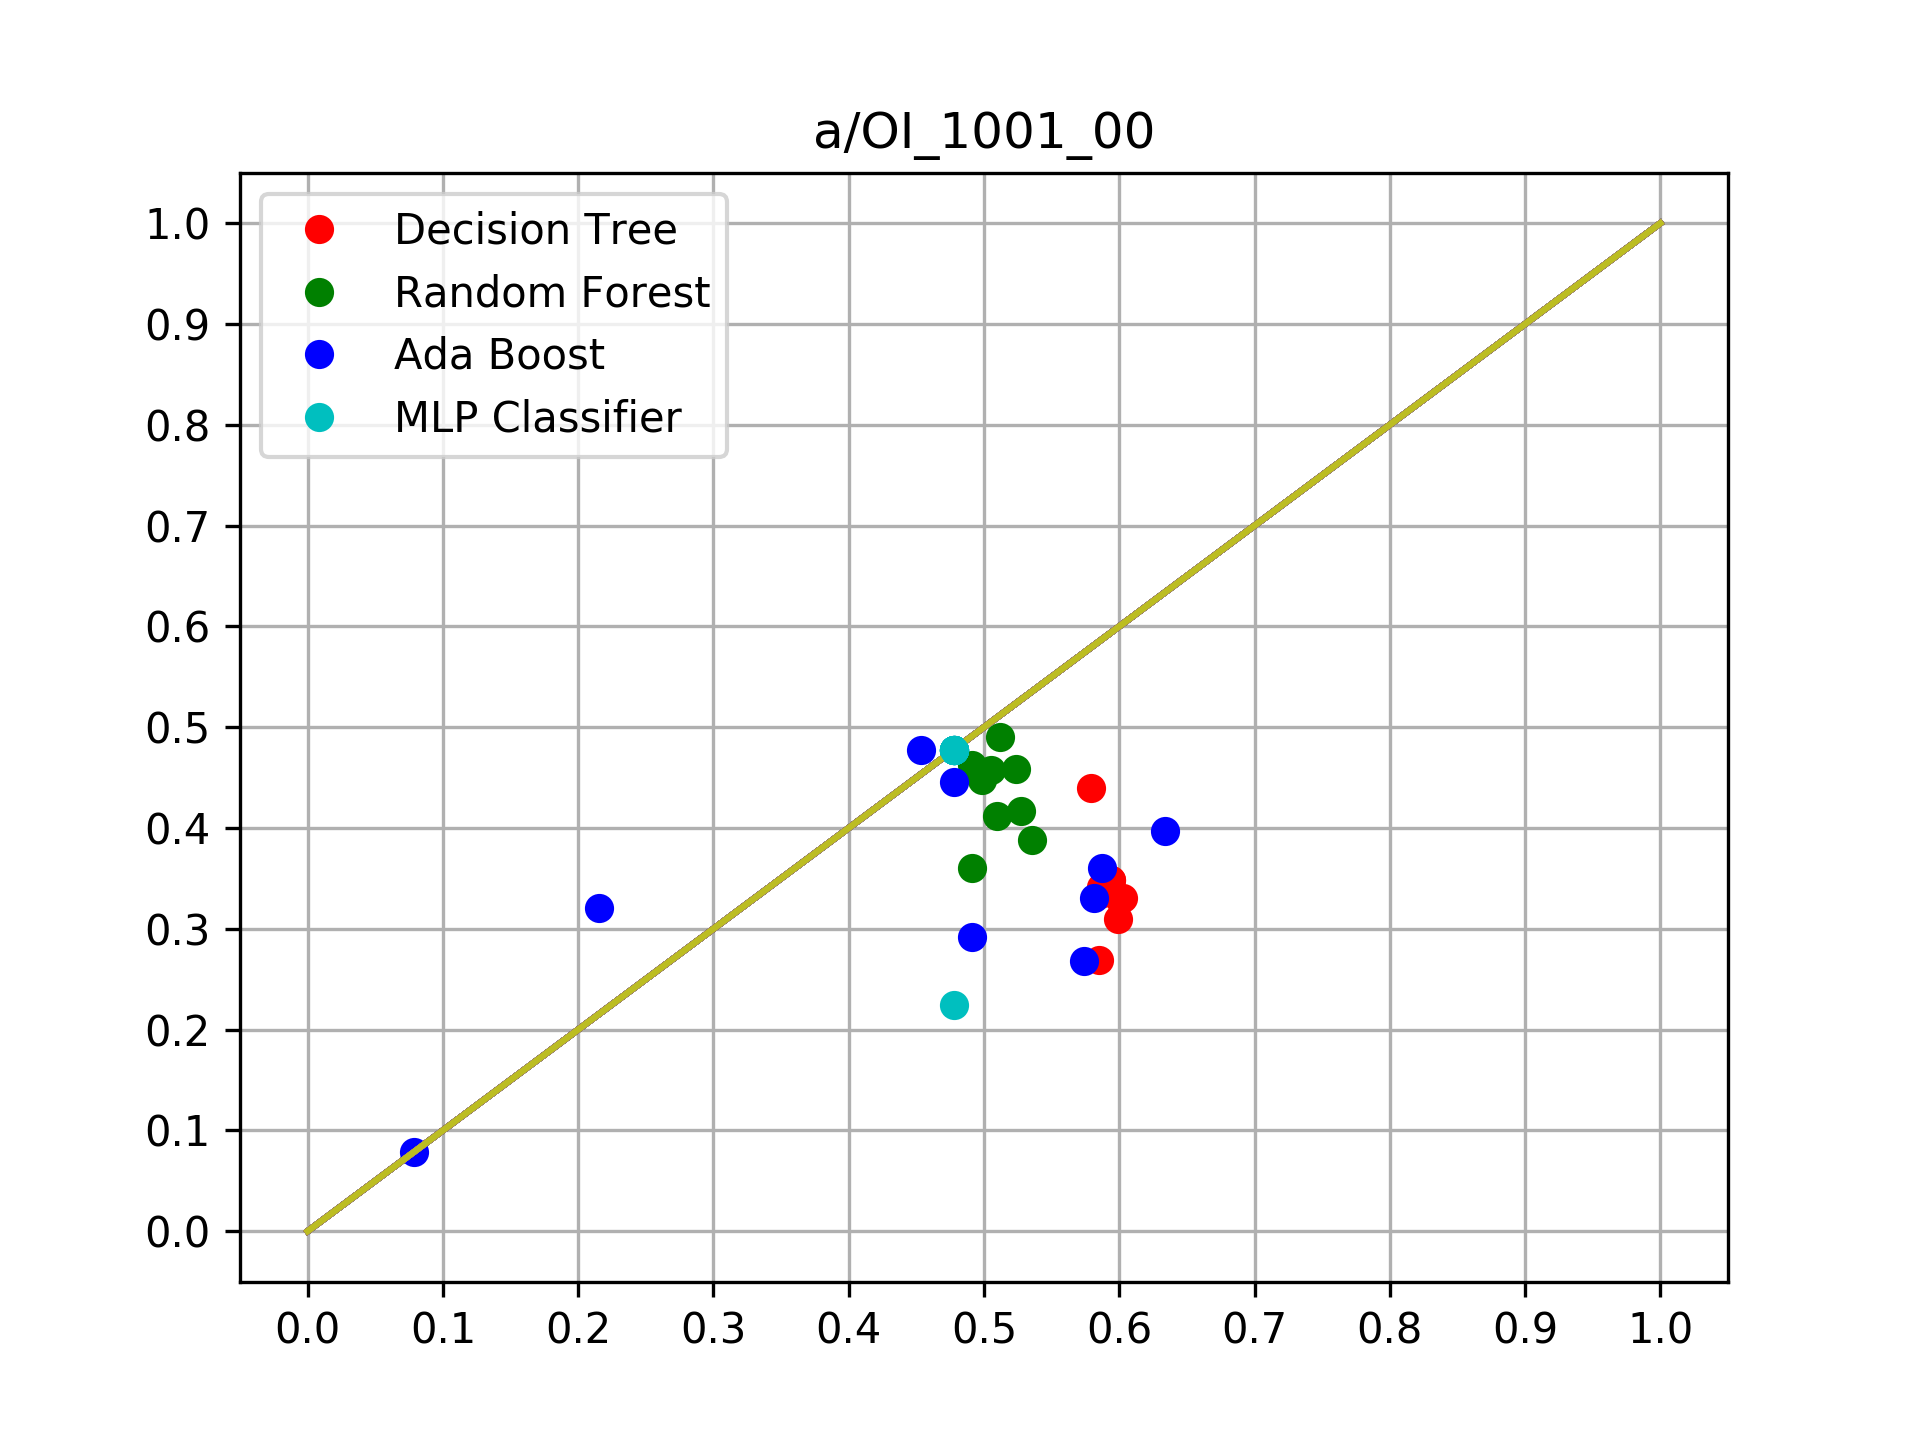
\includegraphics[trim={1cm 0.8cm 1cm 1.37cm},clip,width=0.24\textwidth]
{images/Health_DCGAN_12.png}}
\subfigure[The best of ARX,Health]{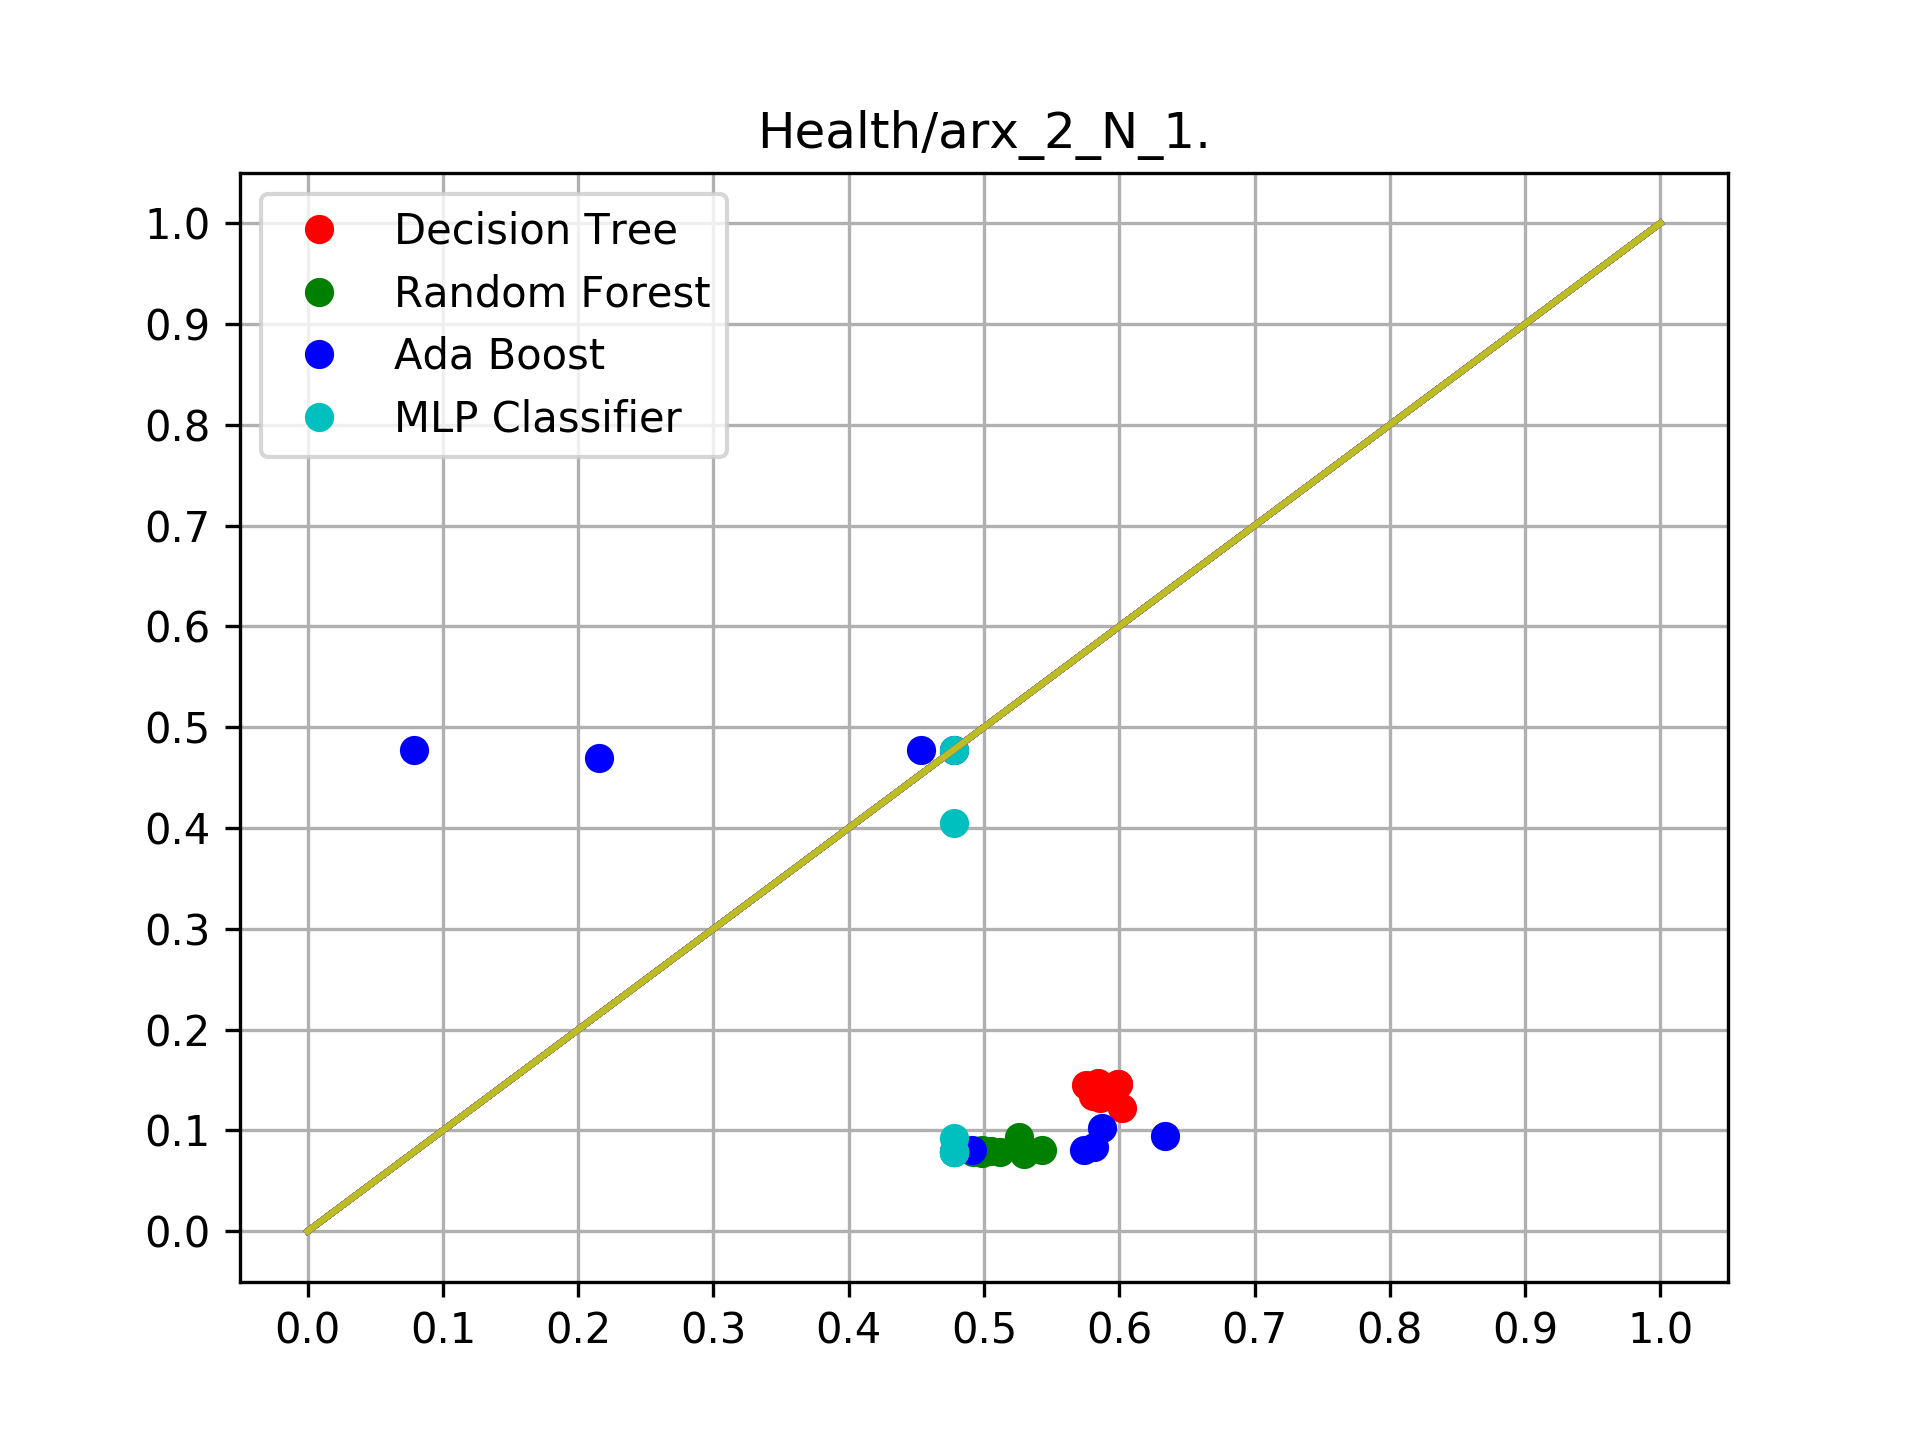
\includegraphics[trim={1cm 0.8cm 1cm 1.37cm},clip,width=0.24\textwidth]
{images/Health_ARX_17.png}}
\subfigure[The best of sdcMicro,Health]{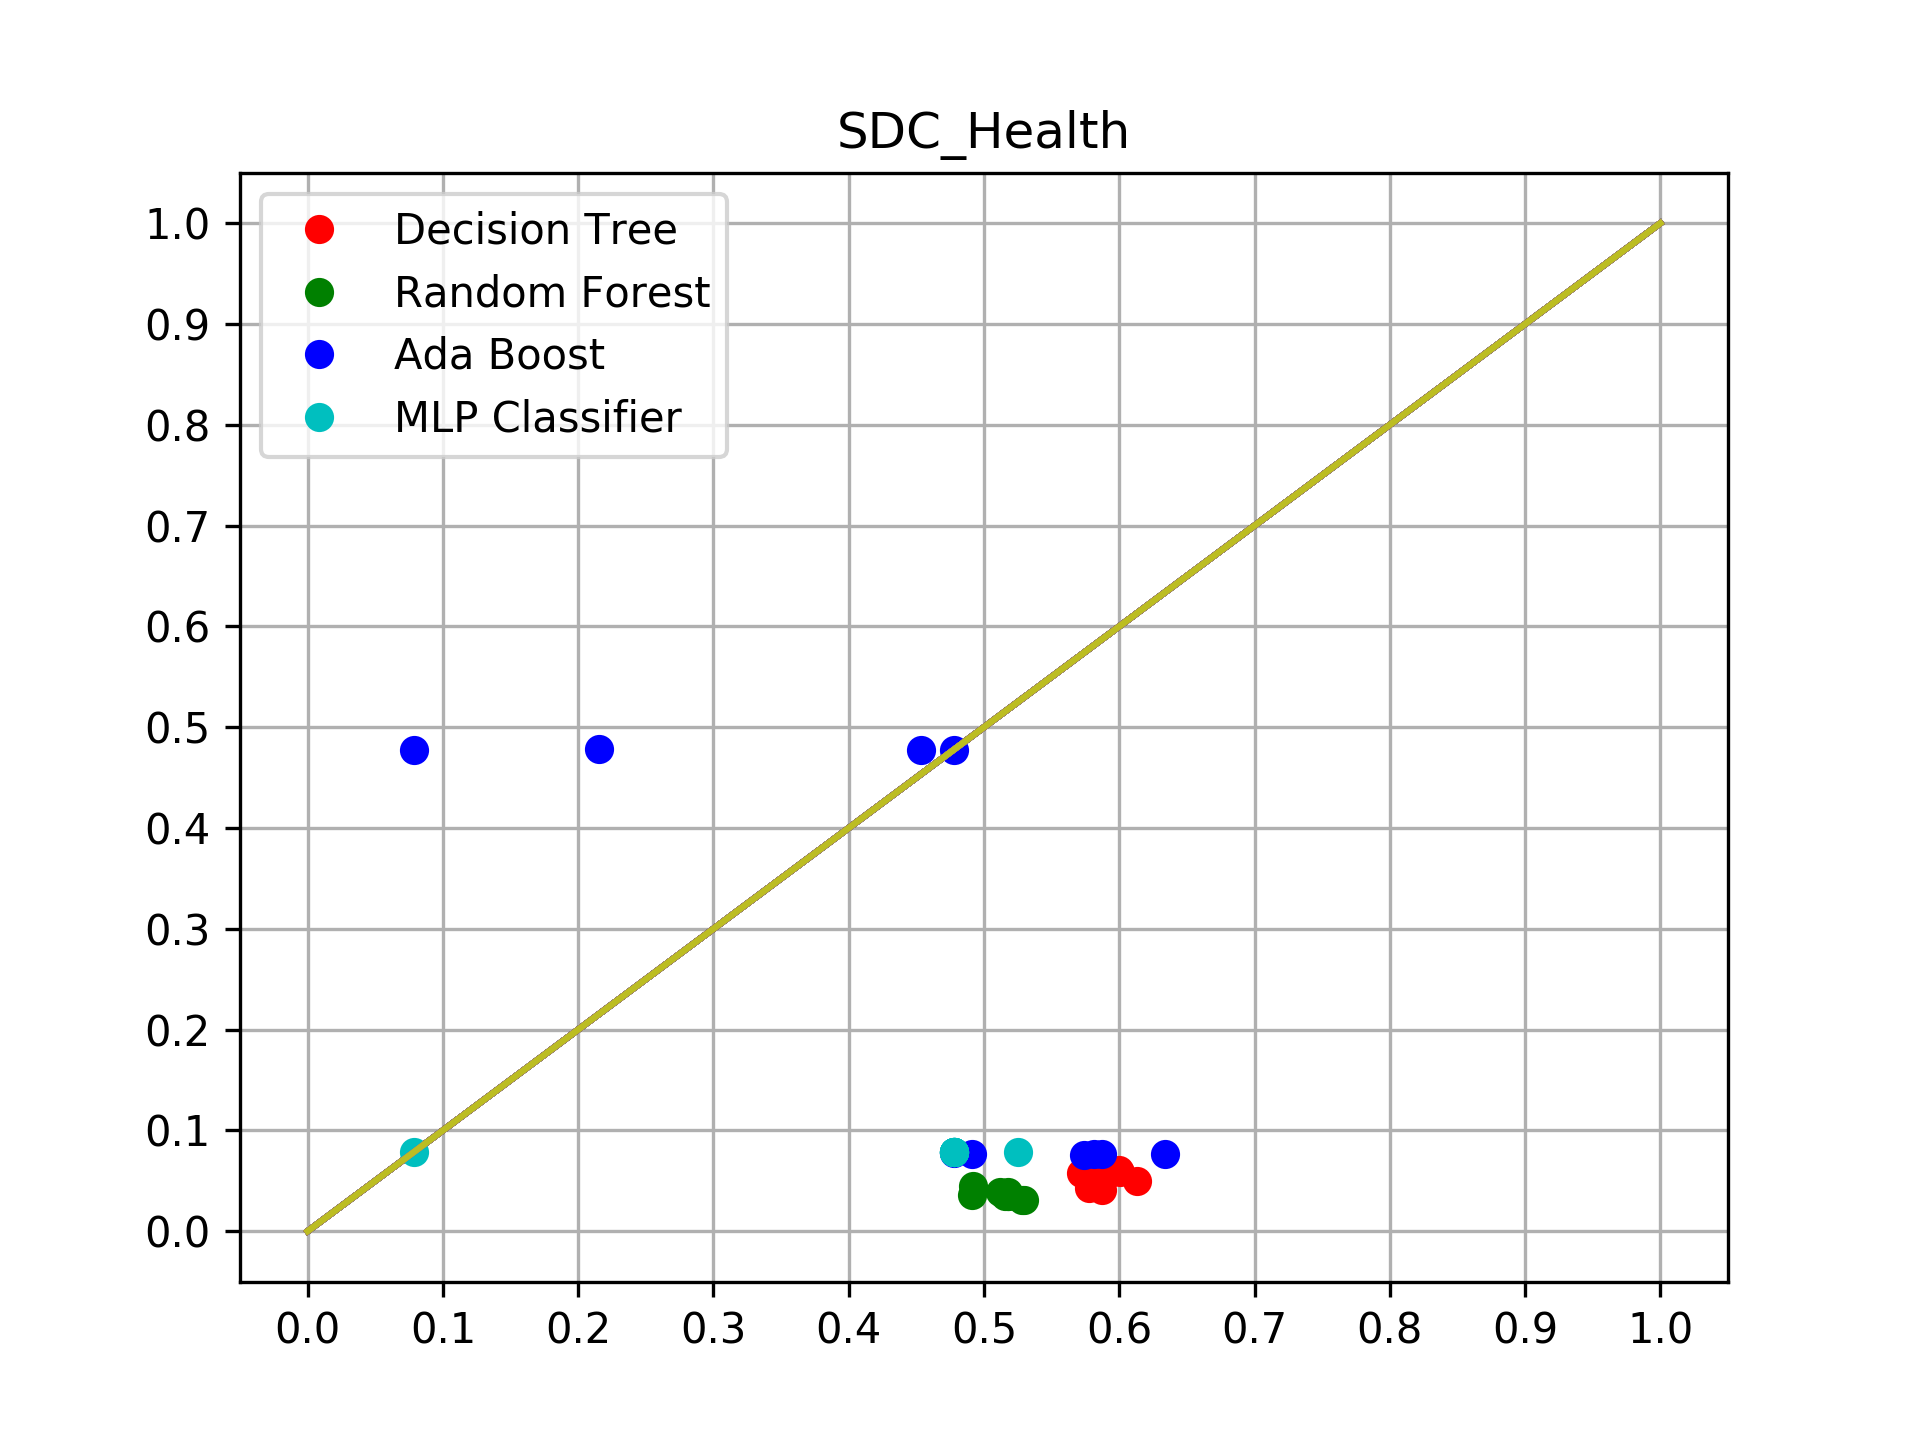
\includegraphics[trim={1cm 0.8cm 1cm 1.37cm},clip,width=0.24\textwidth]
{images/Health_SDC_1.png}}\\

\vspace{-1em}
\subfigure[Ours,low-privacy,Airline]{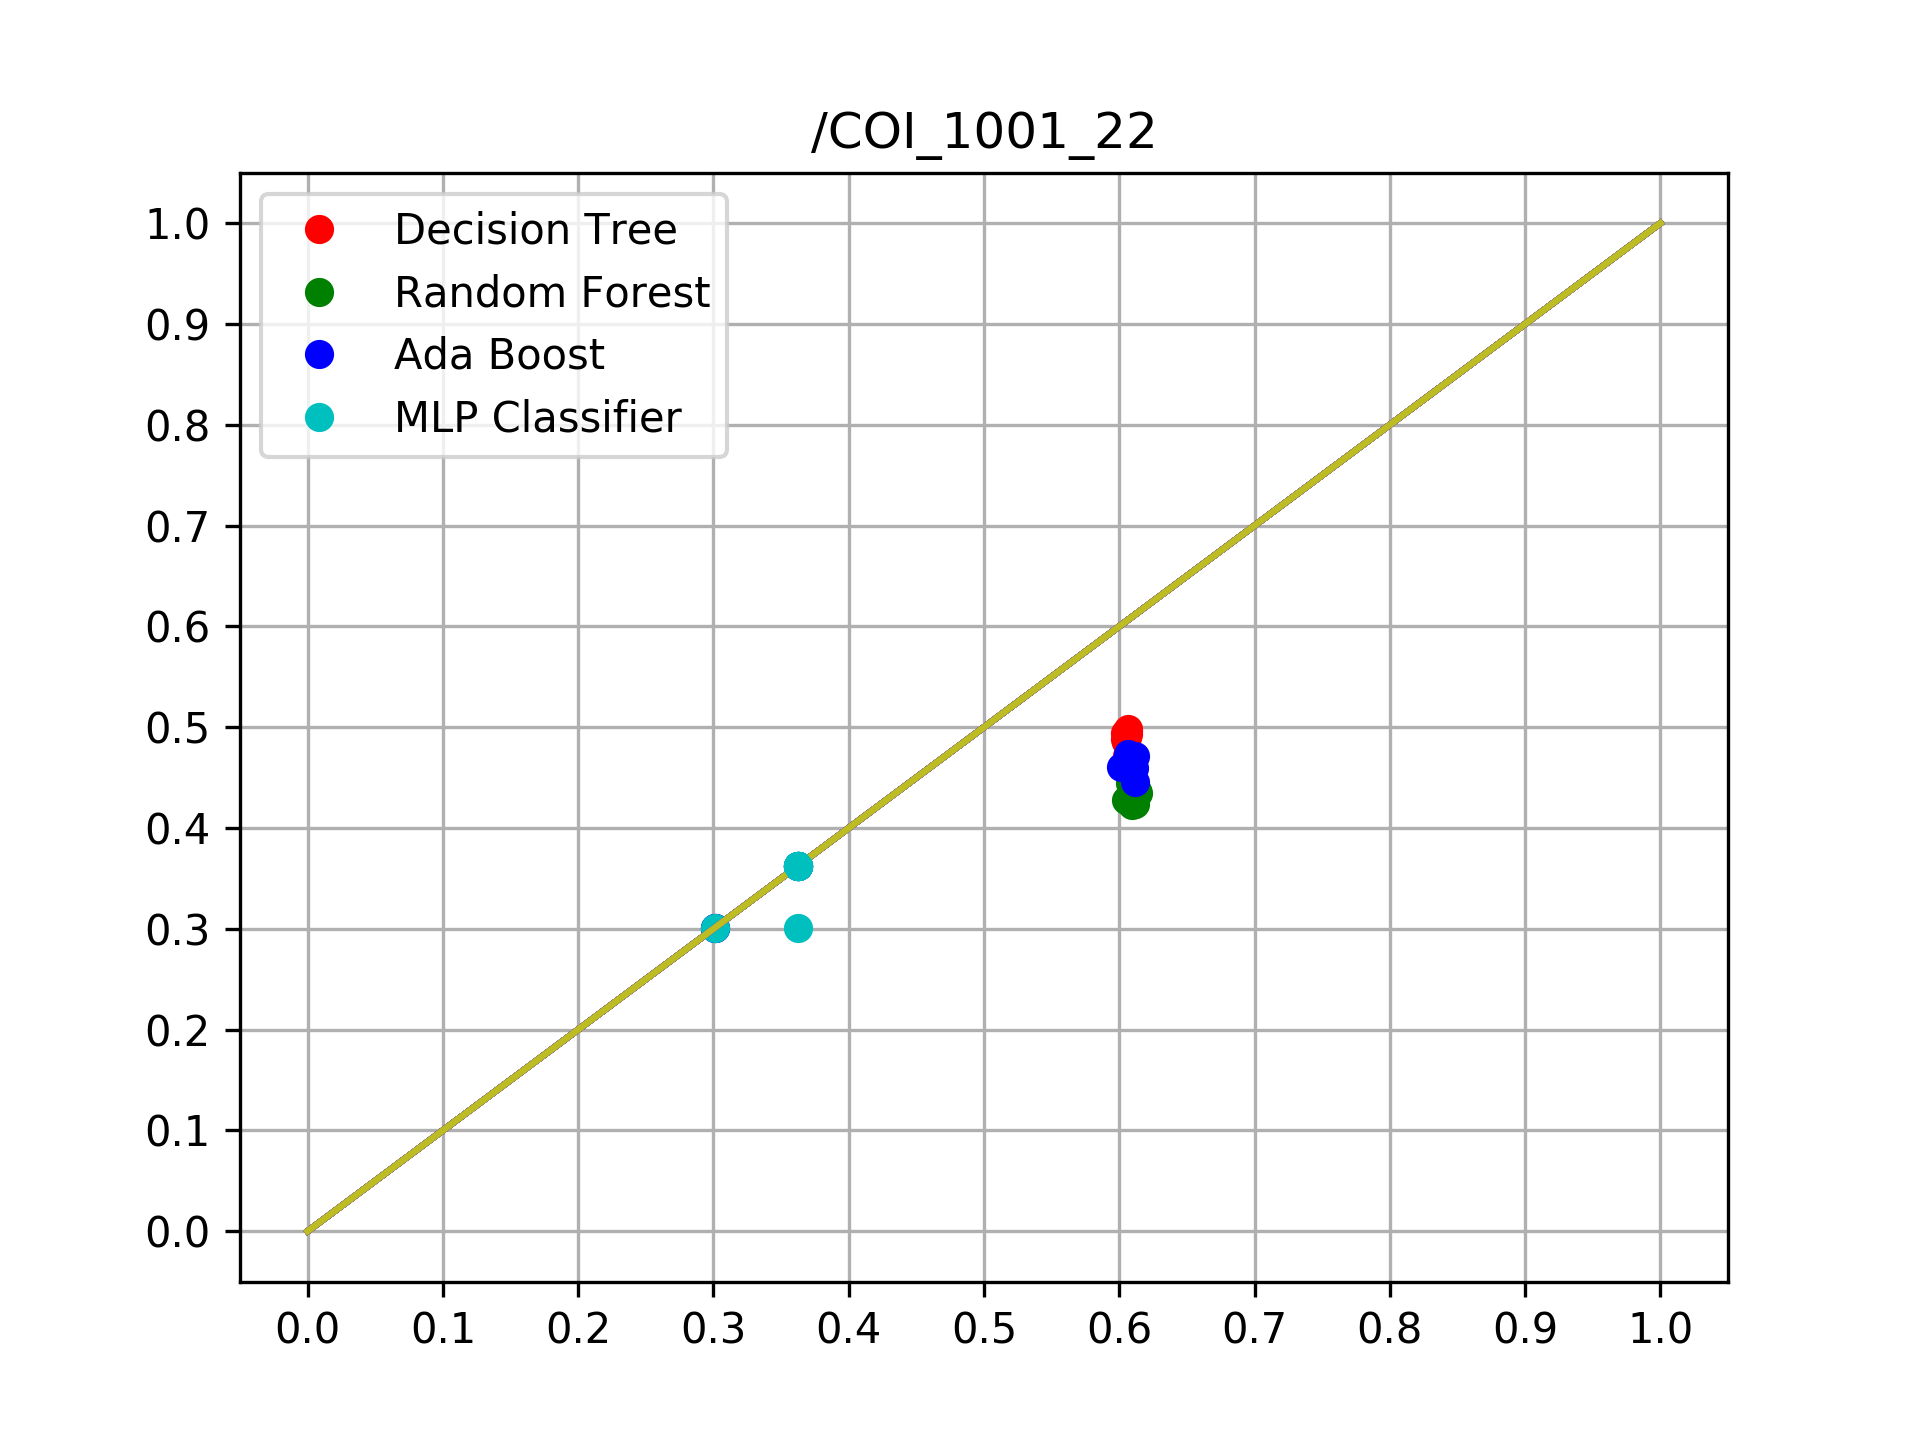
\includegraphics[trim={1cm 0.8cm 1cm 1.37cm},clip,width=0.24\textwidth]
{images/Ticket_DCGAN_10.png}}
\subfigure[Ours,high-privacy,Airline]{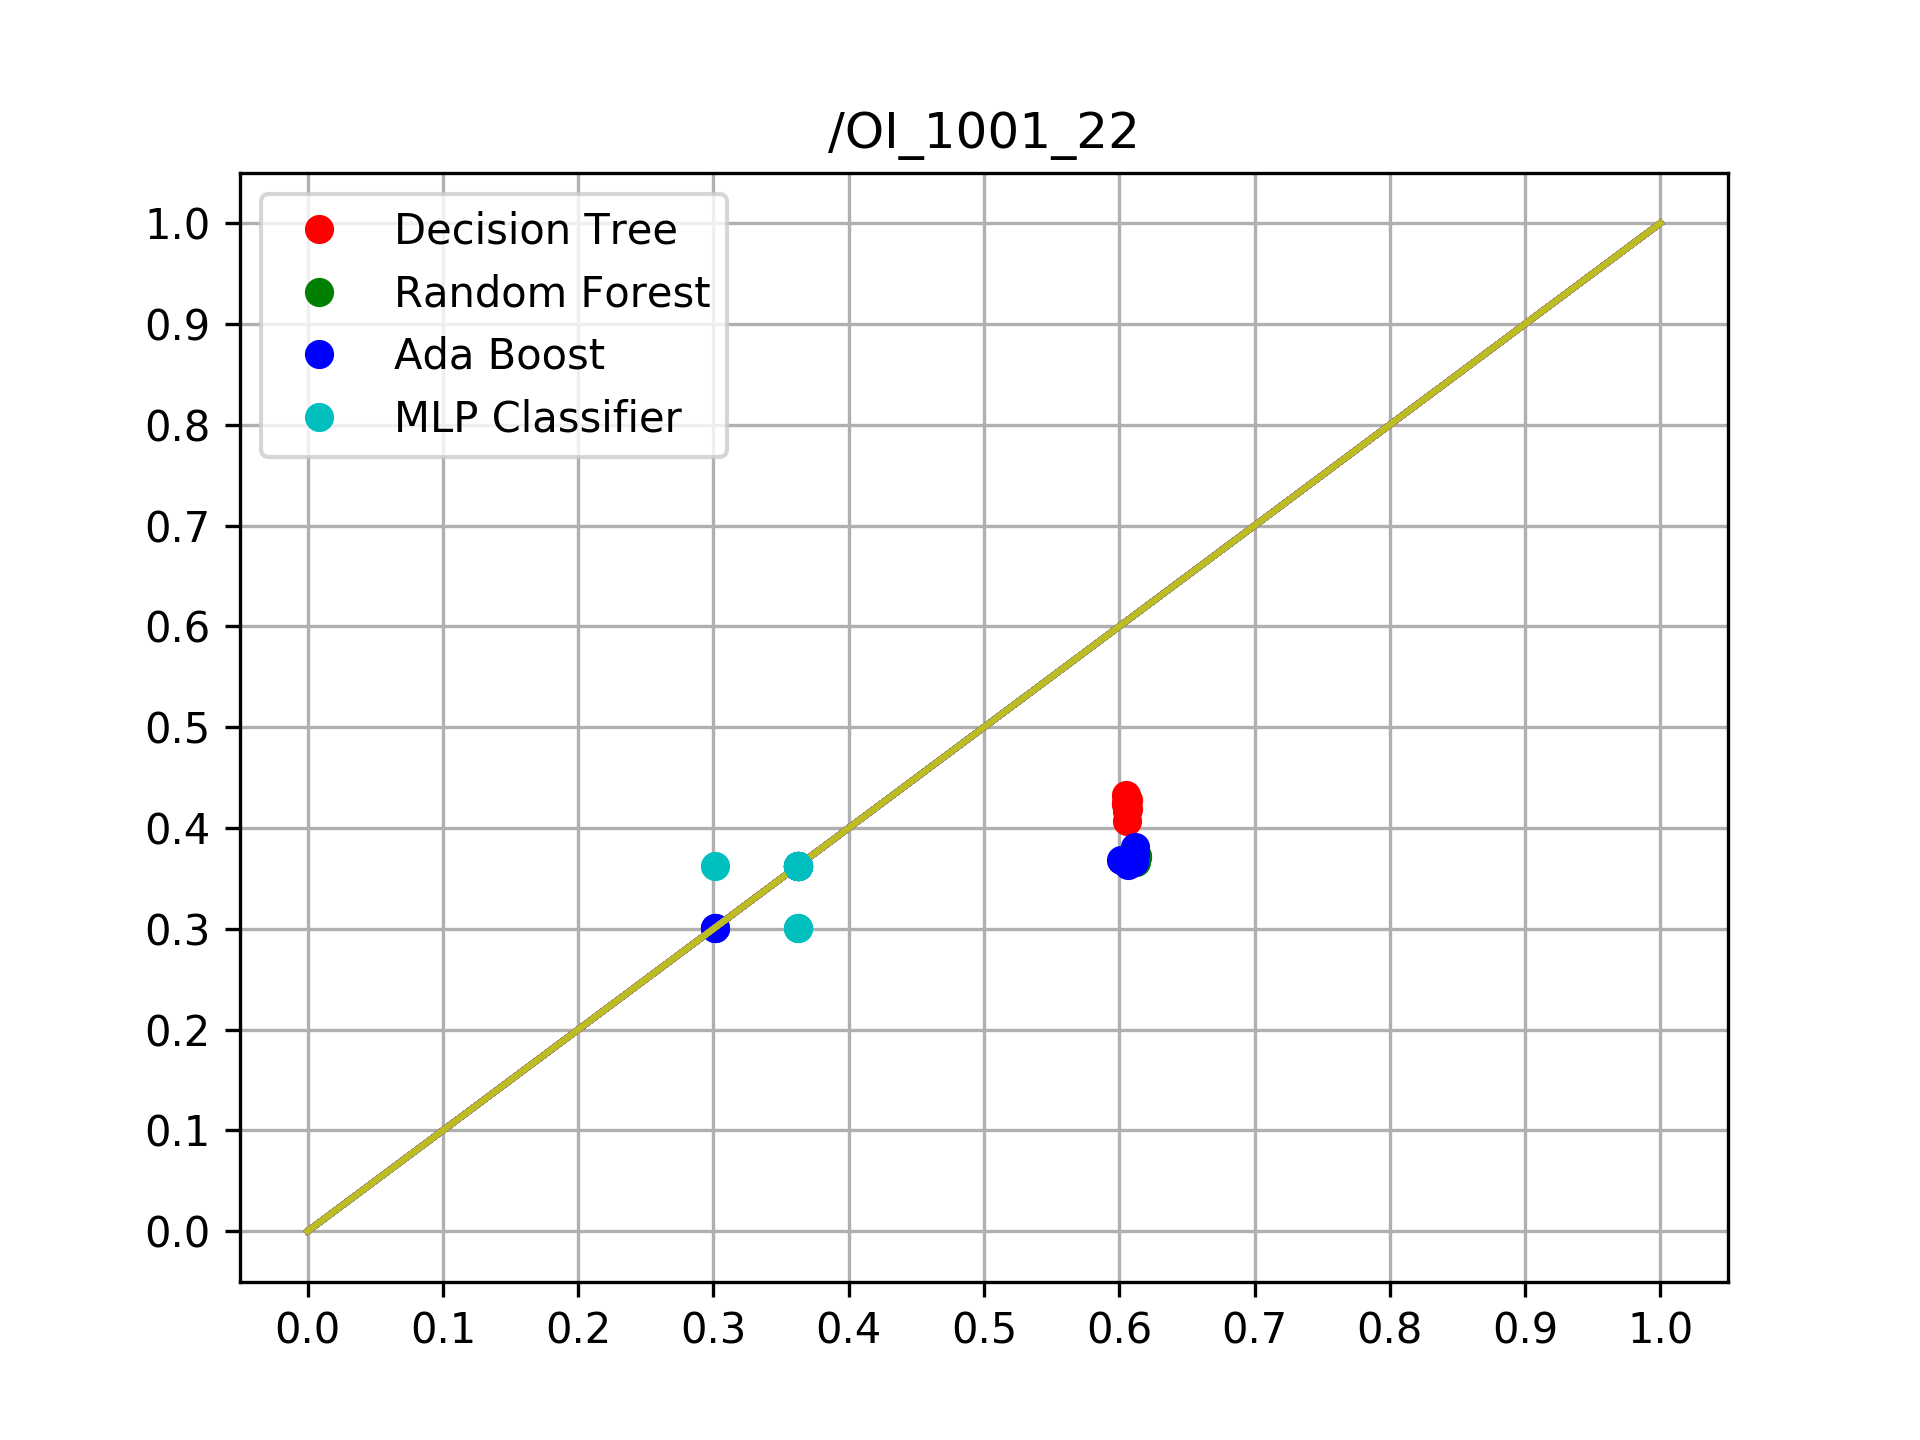
\includegraphics[trim={1cm 0.8cm 1cm 1.37cm},clip,width=0.24\textwidth]
{images/Ticket_DCGAN_15.png}}
\subfigure[The best of ARX,Airline]{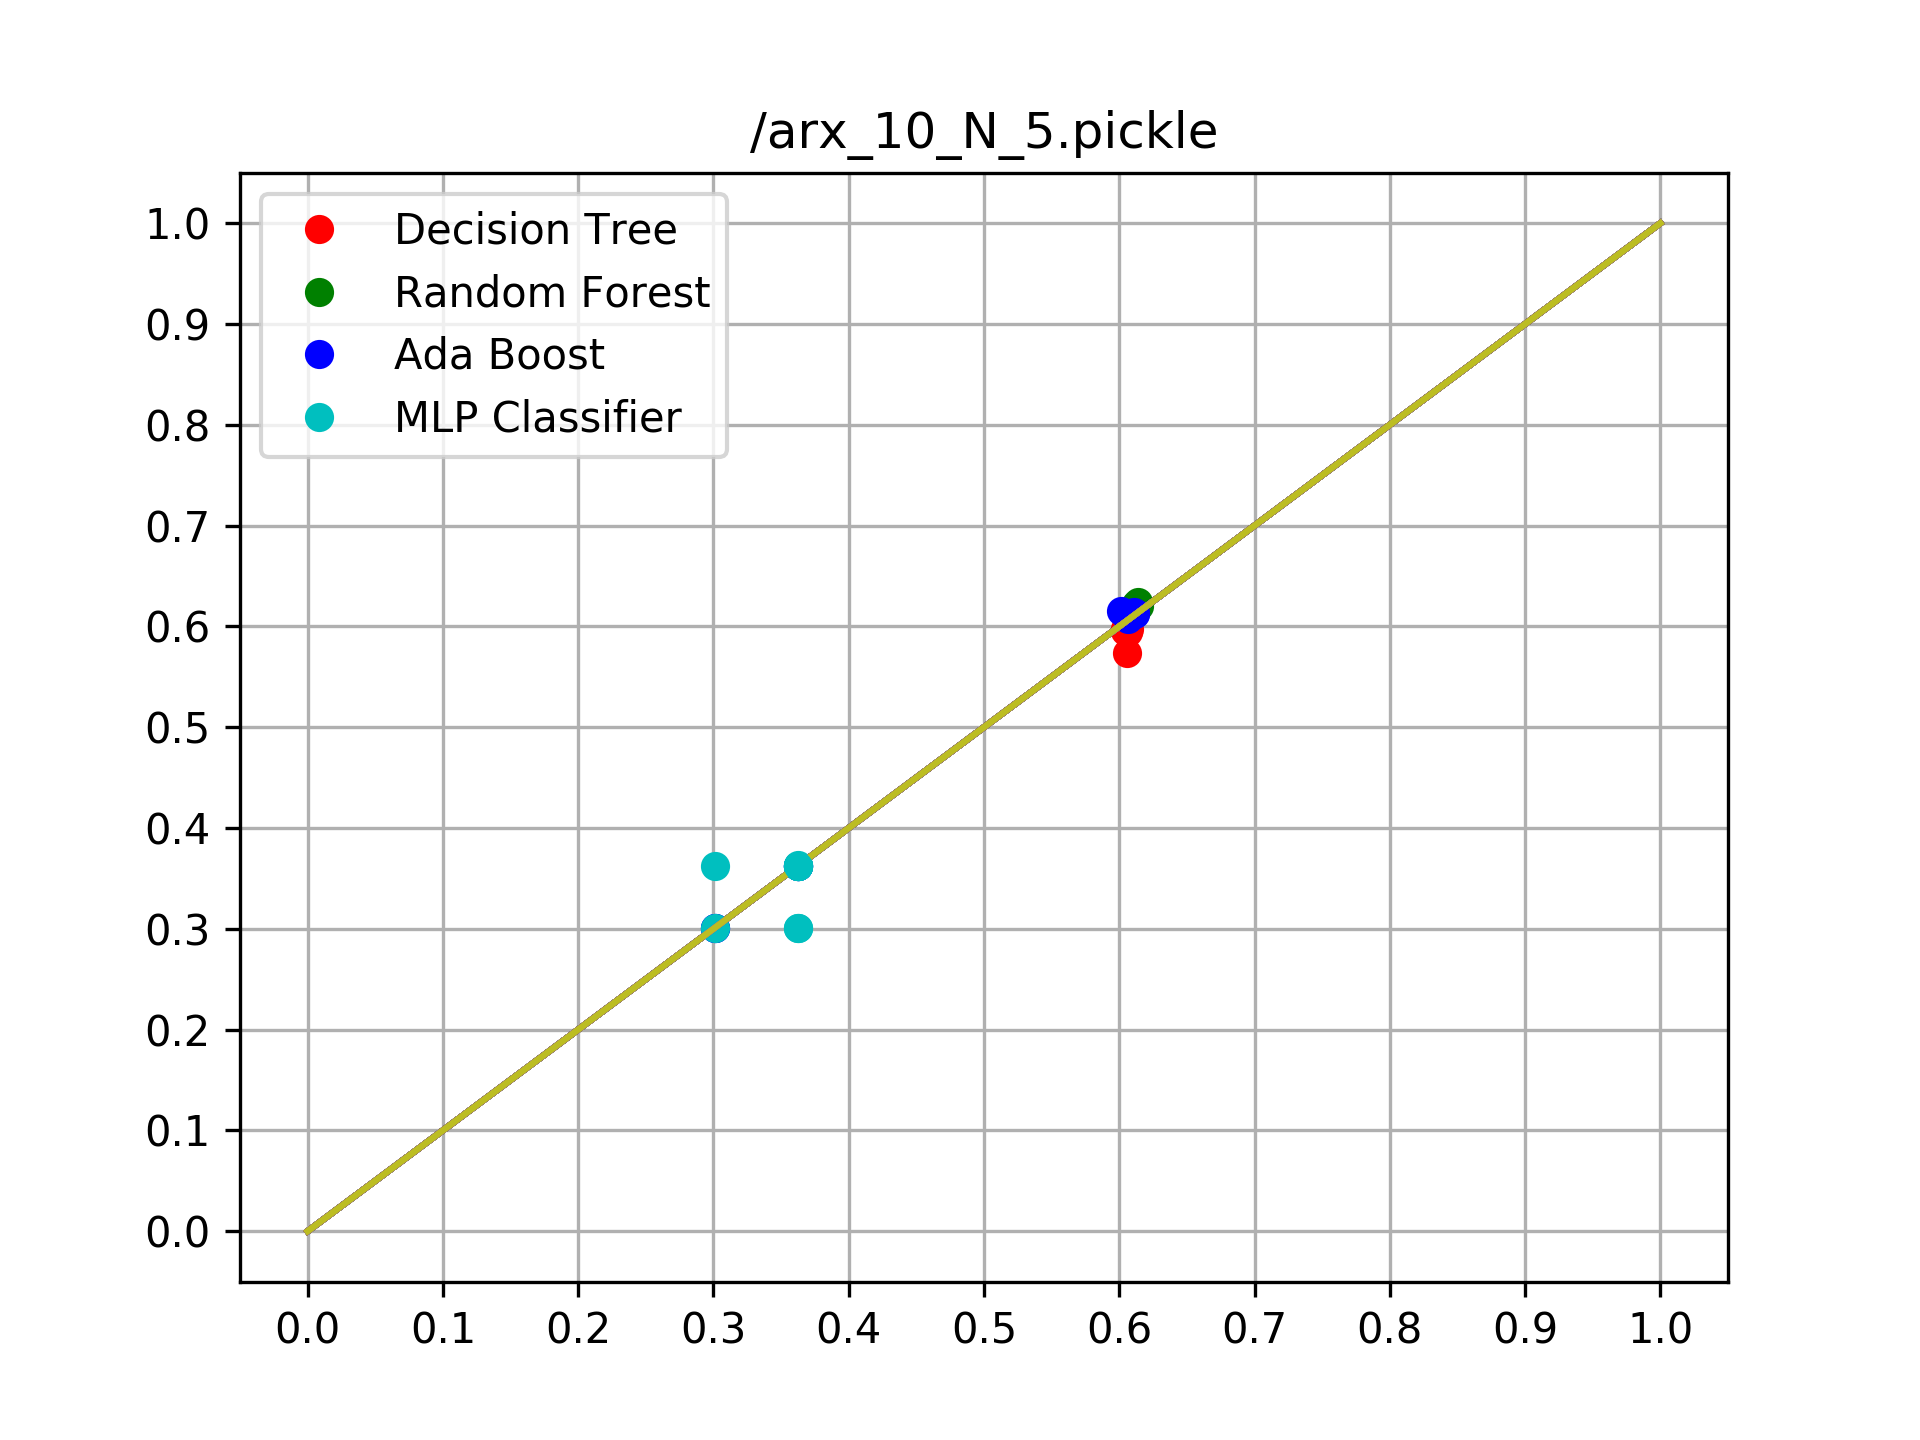
\includegraphics[trim={1cm 0.8cm 1cm 1.37cm},clip,width=0.24\textwidth]
{images/Ticket_ARX_4.png}}
\subfigure[The best of sdcMicro,Airline]{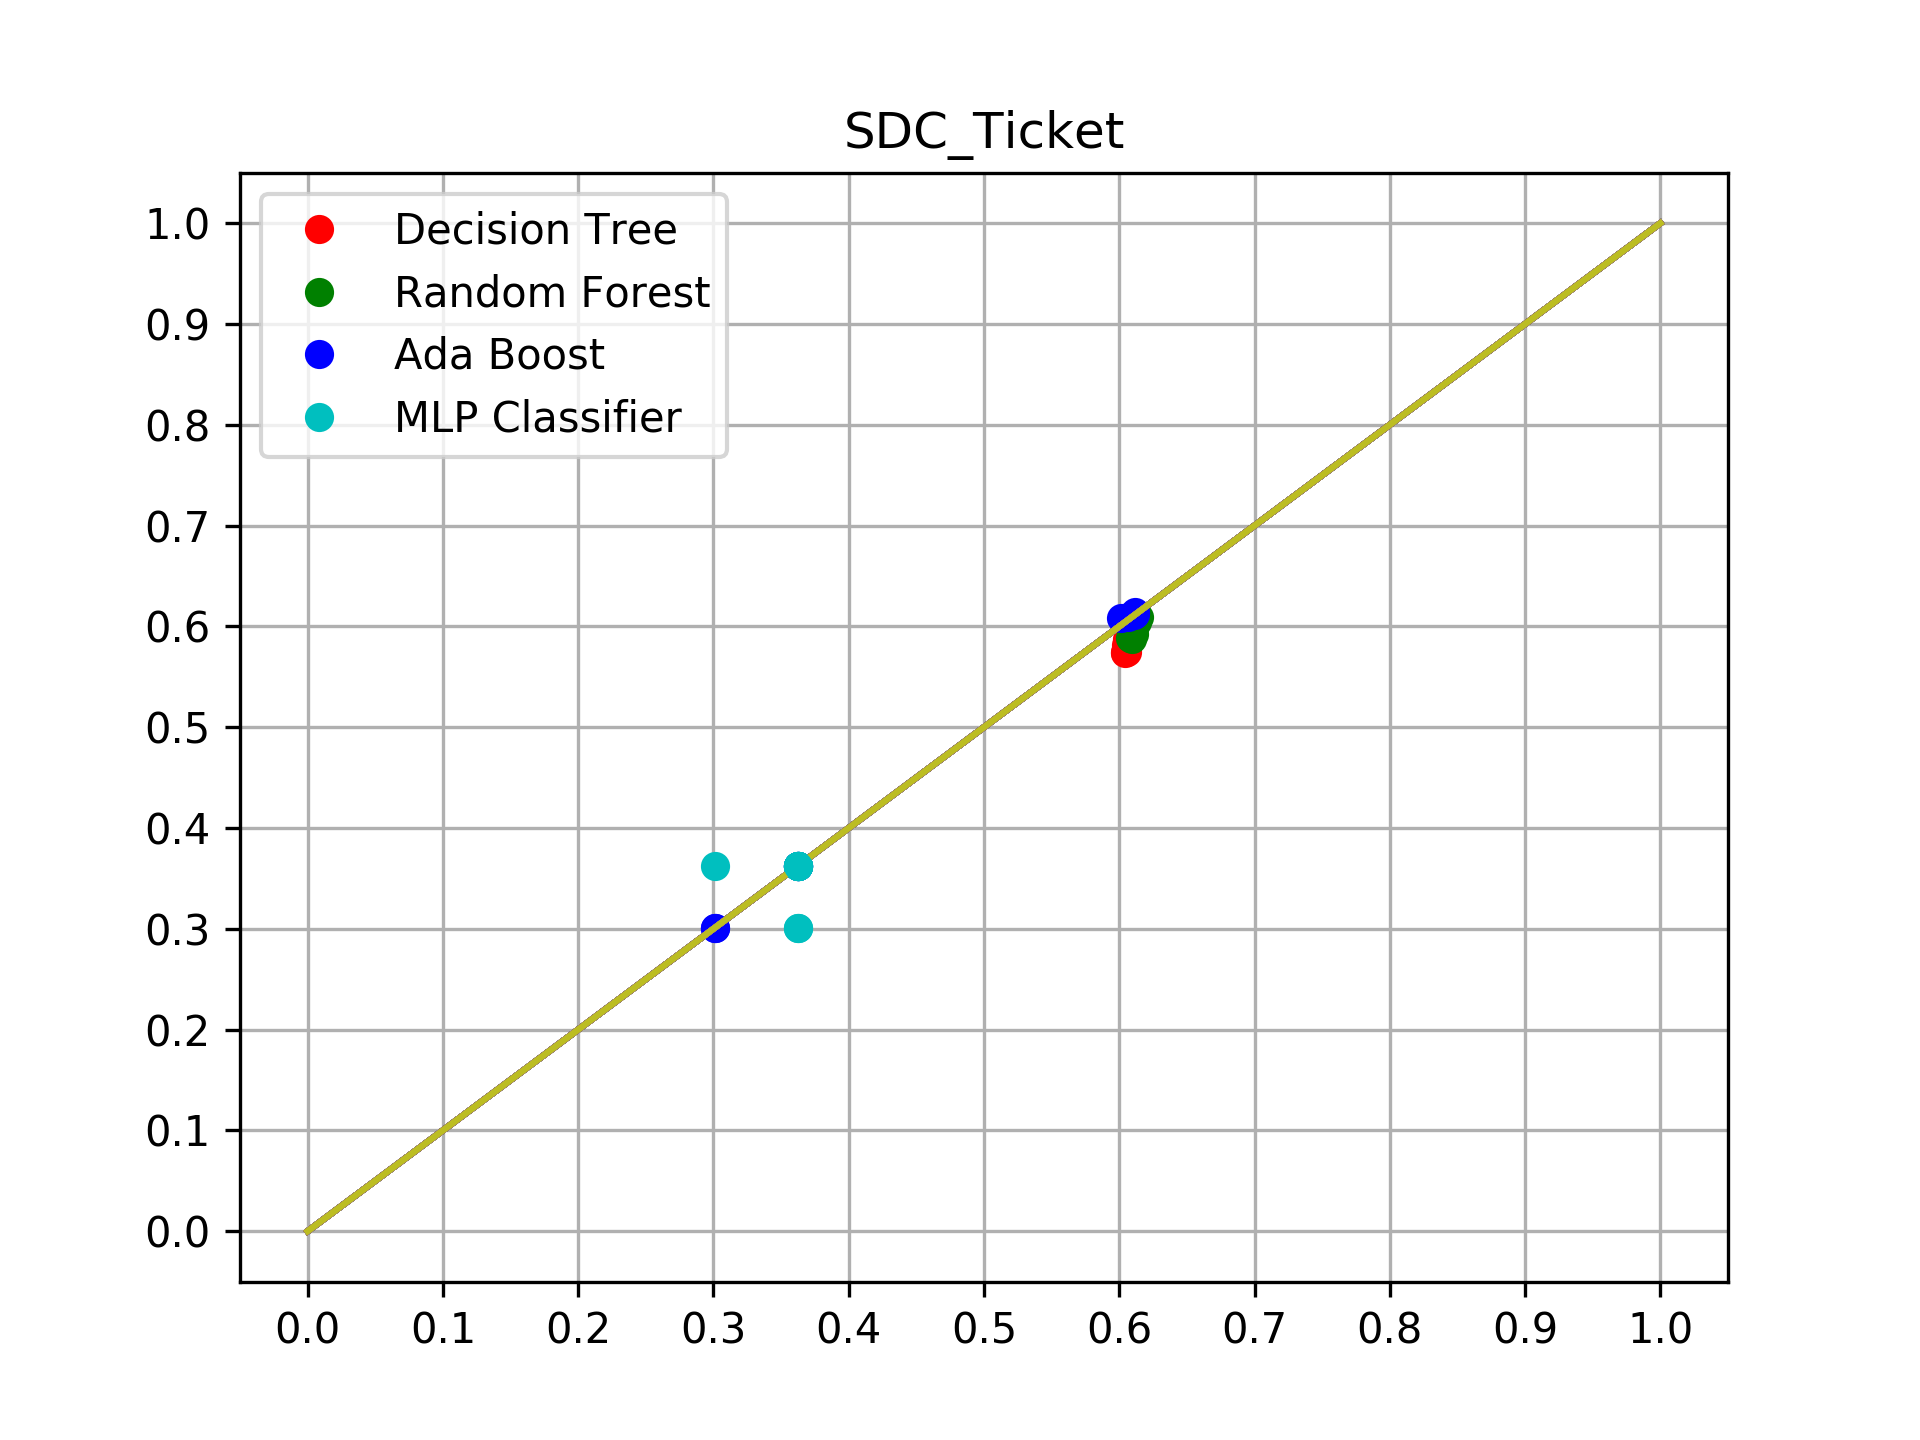
\includegraphics[trim={1cm 0.8cm 1cm 1.37cm},clip,width=0.24\textwidth]
{images/Ticket_SDC_1.png}}\\

\vspace{-1em}
\caption{Classification score similarity of ARX, sdcMicro, and table-GAN. We remove DCGAN that did not show reliable performance for space limitations. We plot $(x,y)$ after fixing a classification algorithm and its parameter, where $x$ is the F-1 score of the algorithm trained with the original table and $y$ is the F-1 score of the algorithm trained with an anonymized\slash perturbed\slash synthesized table. We test 4 algorithms and 10 parameters for each algorithm. Points on the diagonal line (i.e., $x=y$) mean perfect model compatibility. Only our table-GAN shows reliable model compatibility in all datasets.}\label{fig:ss}
\end{figure*}

\begin{figure*}[t]
\centering
\subfigure[Ours,low-privacy,LACity]{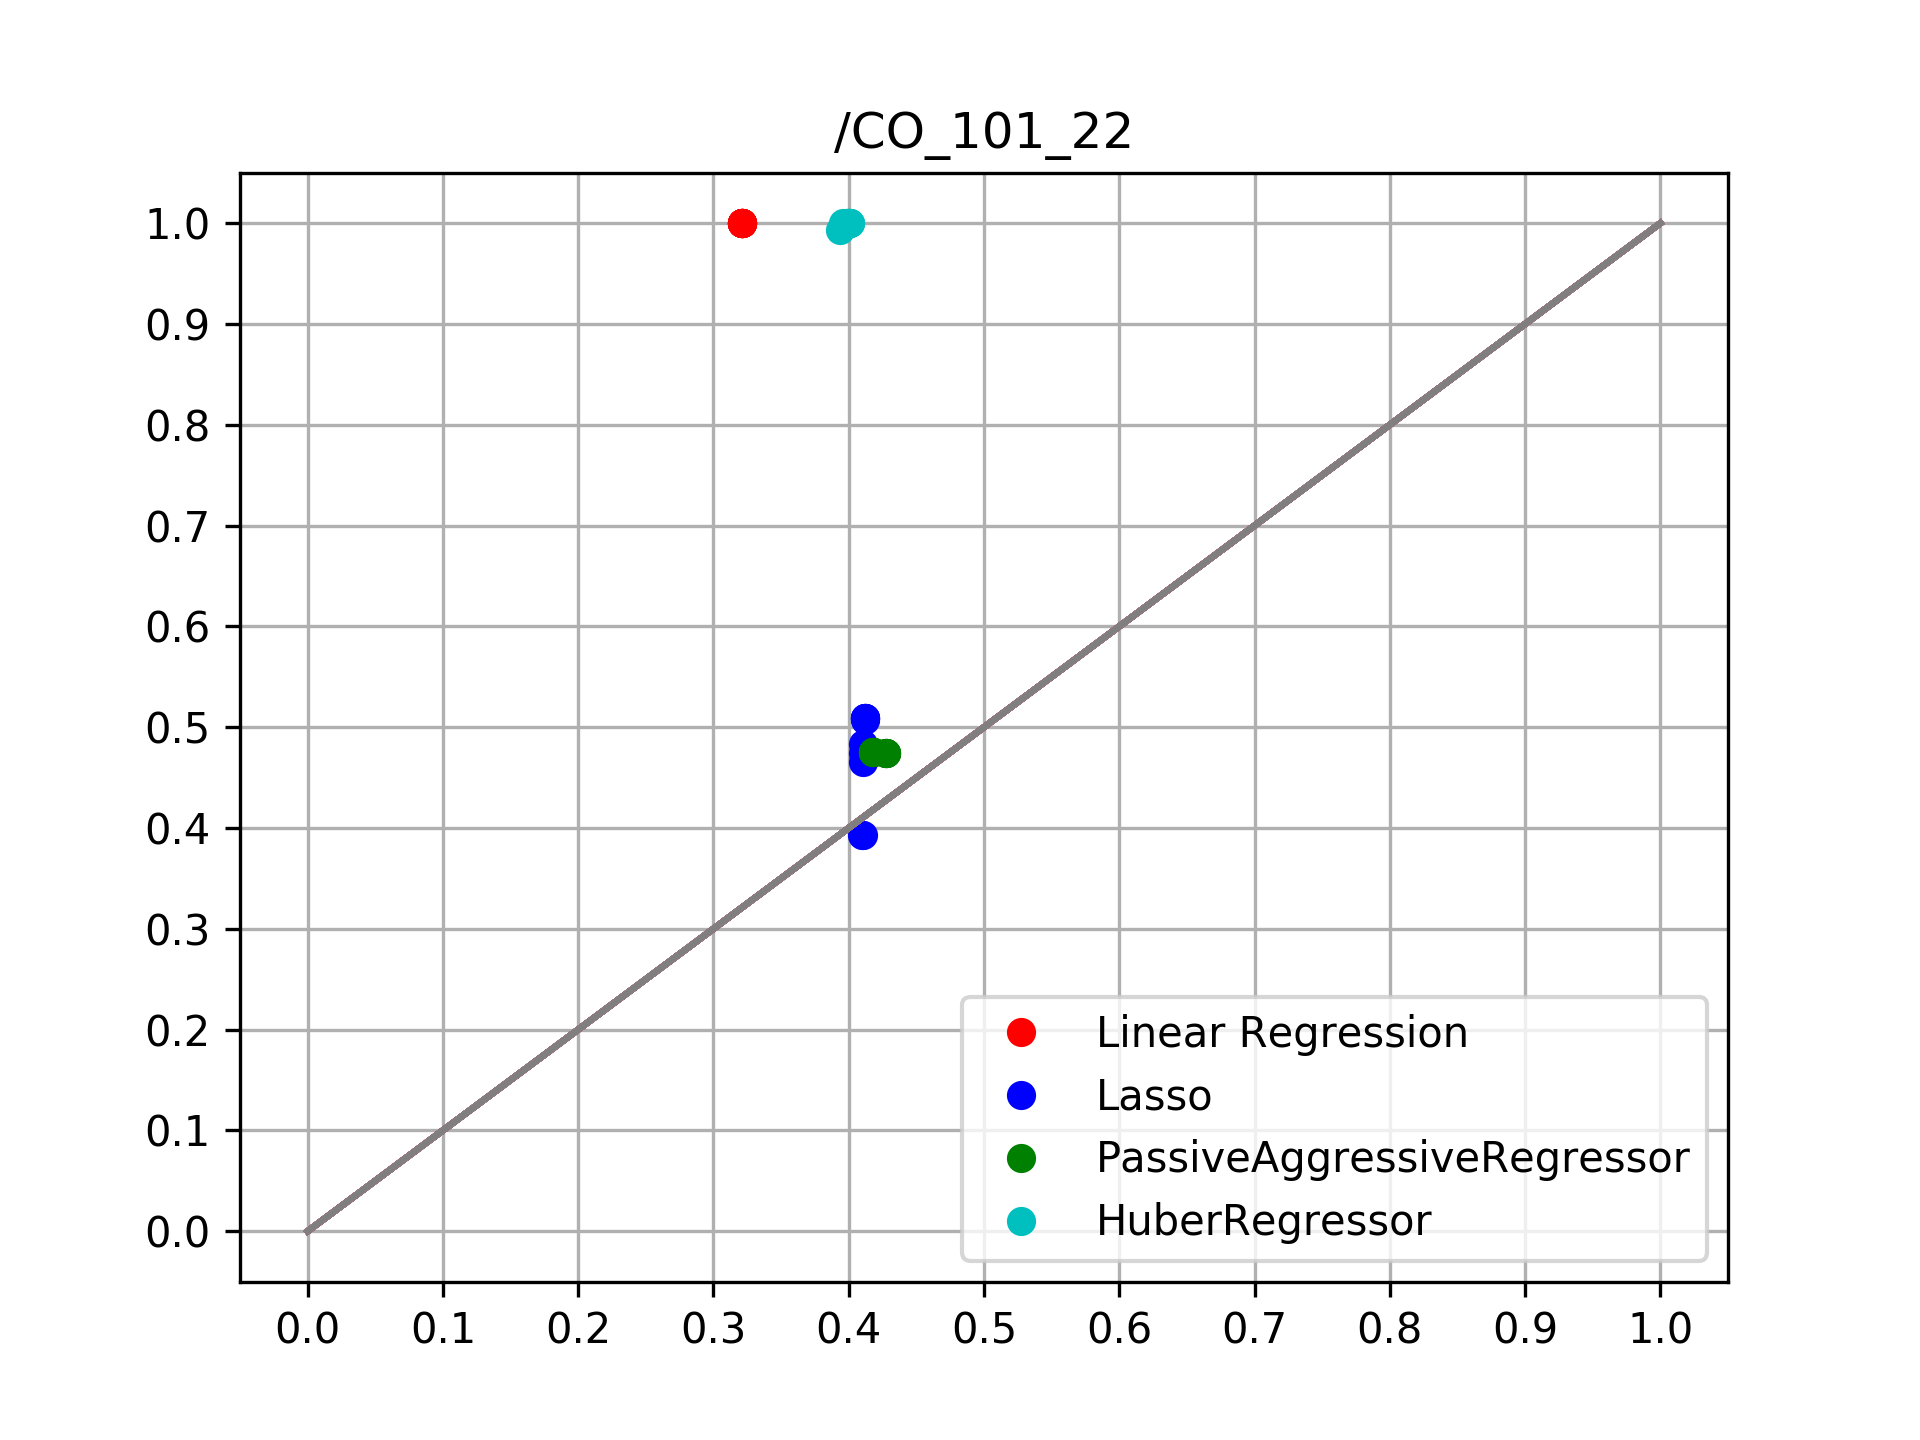
\includegraphics[trim={1cm 0.8cm 1cm 1.37cm},clip,width=0.24\textwidth]{images/Regression_DCGAN_LACity_2.png}}
\subfigure[Ours,high-privacy,LACity]{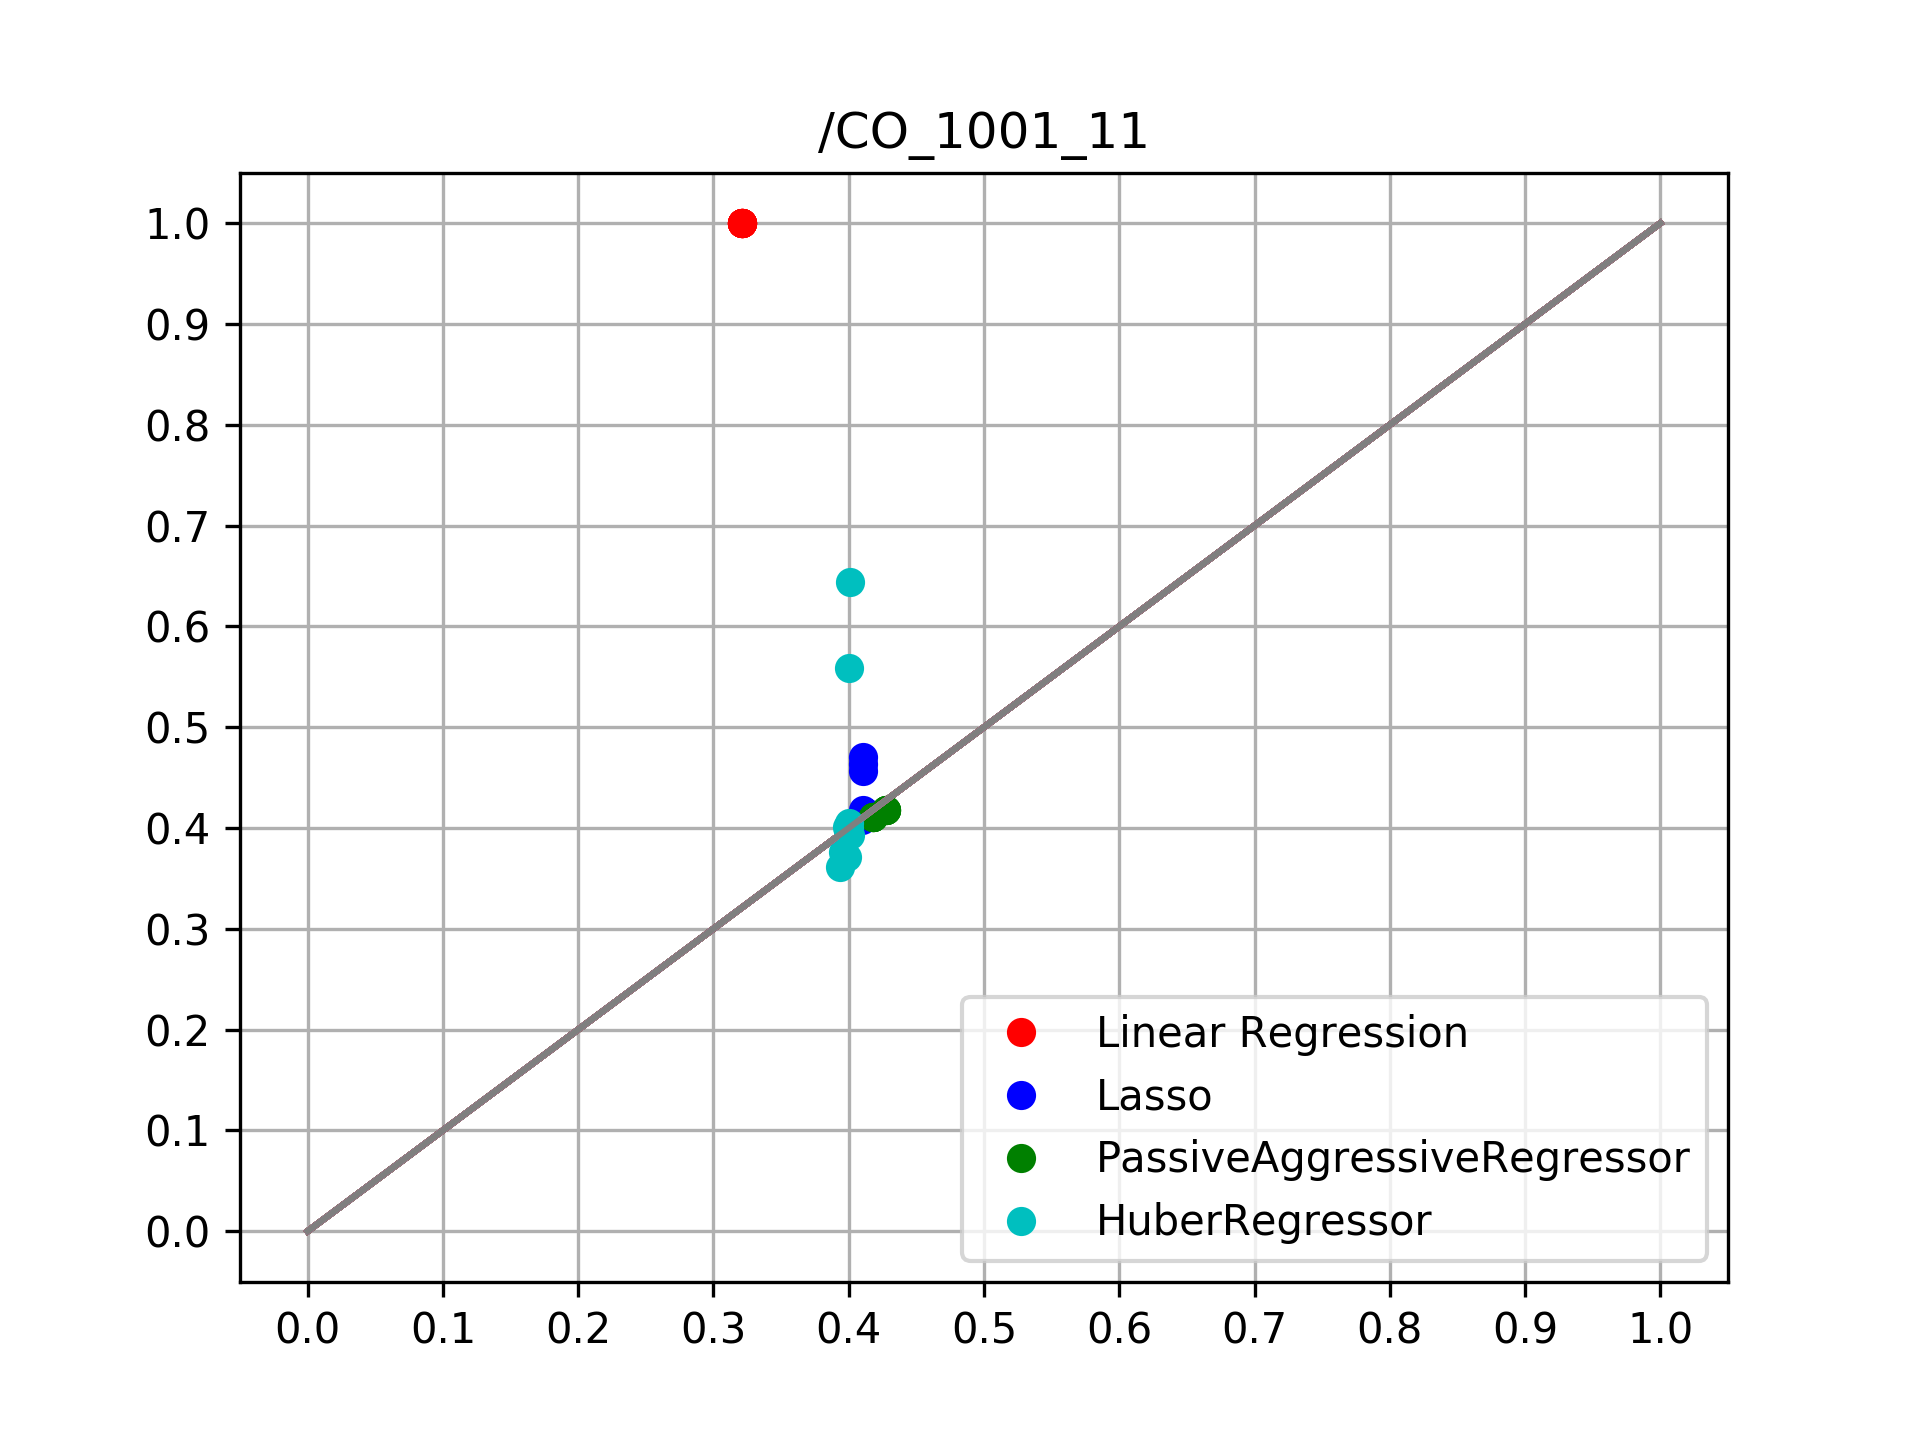
\includegraphics[trim={1cm 0.8cm 1cm 1.37cm},clip,width=0.24\textwidth]
{images/Regression_DCGAN_LACity_3.png}}
\subfigure[The best of ARX,LACity]{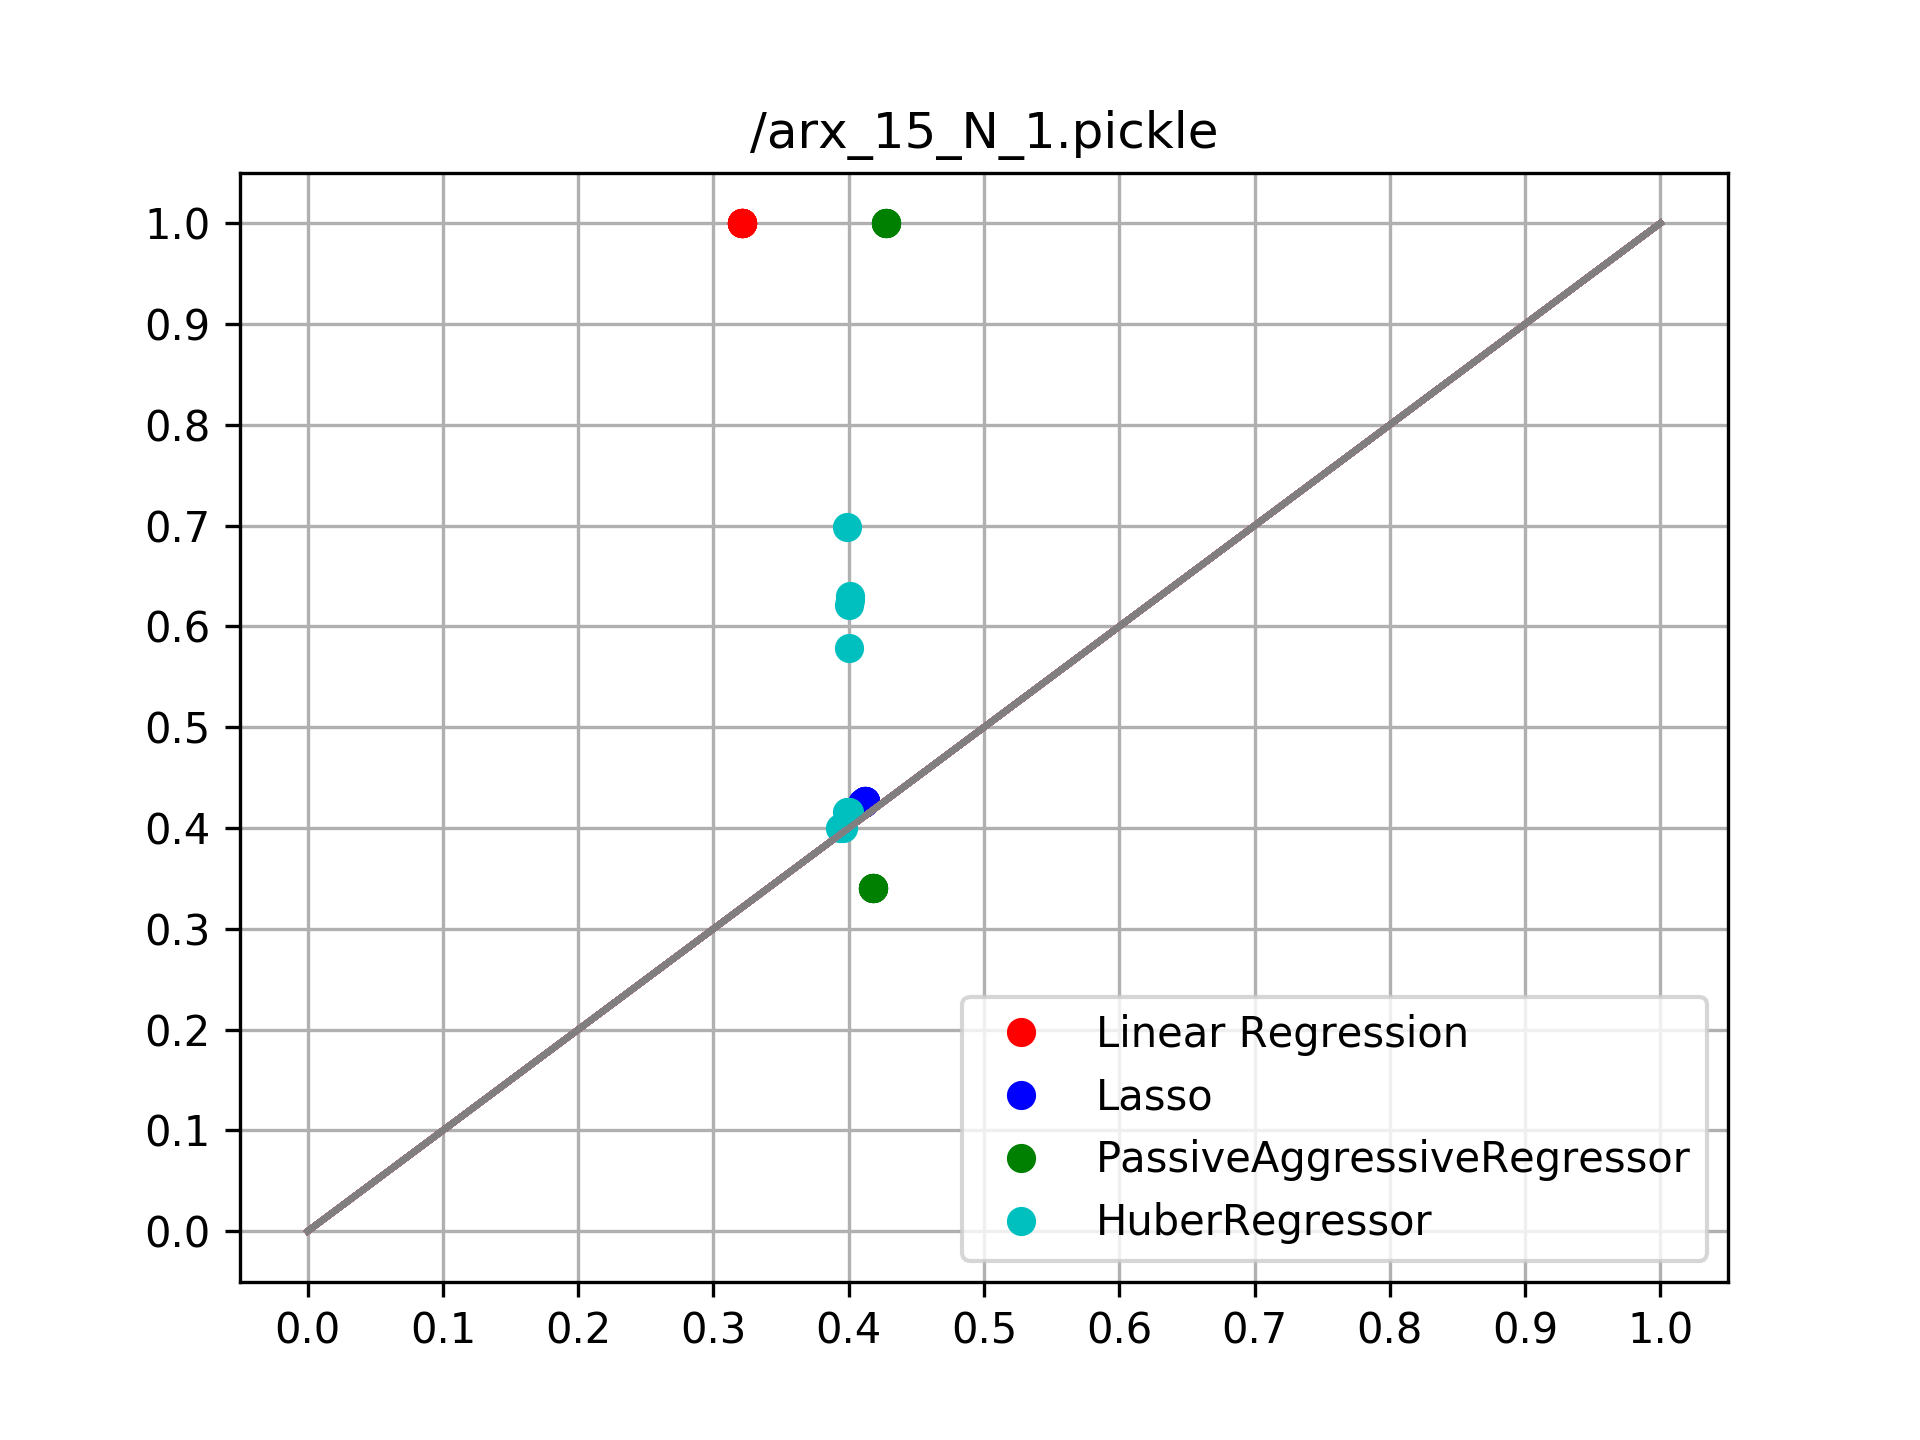
\includegraphics[trim={1cm 0.8cm 1cm 1.37cm},clip,width=0.24\textwidth]{images/Regression_ARX_LACity_36.png}}
\subfigure[The best of sdcMicro,LACity]{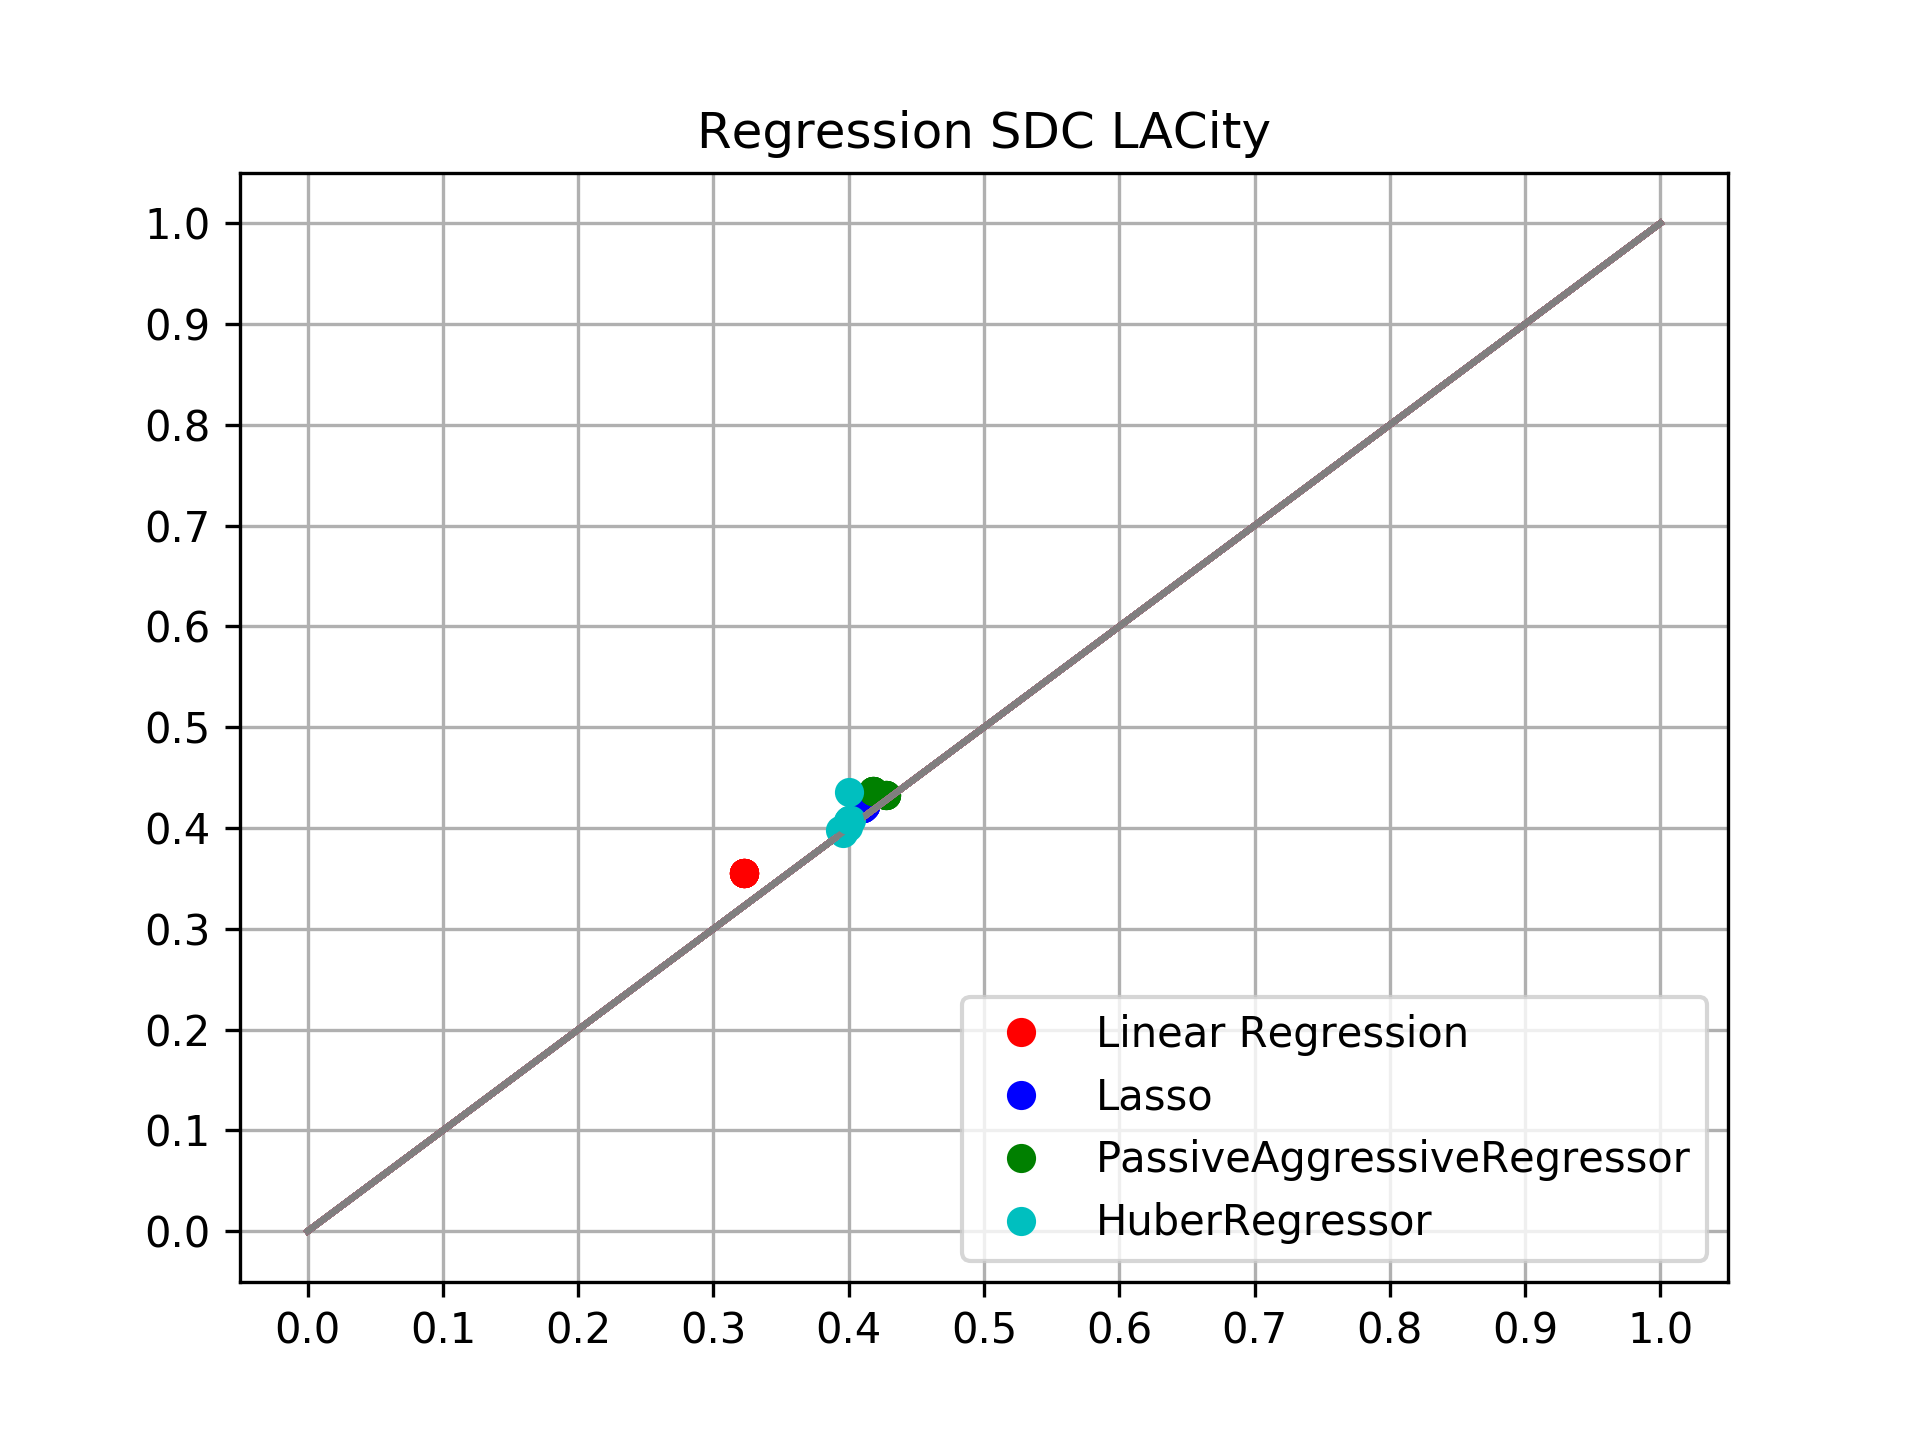
\includegraphics[trim={1cm 0.8cm 1cm 1.37cm},clip,width=0.24\textwidth]{images/Regression_SDC_LACity.png}}\\
\vspace{-1em}

\subfigure[Ours,low-privacy,Adult]{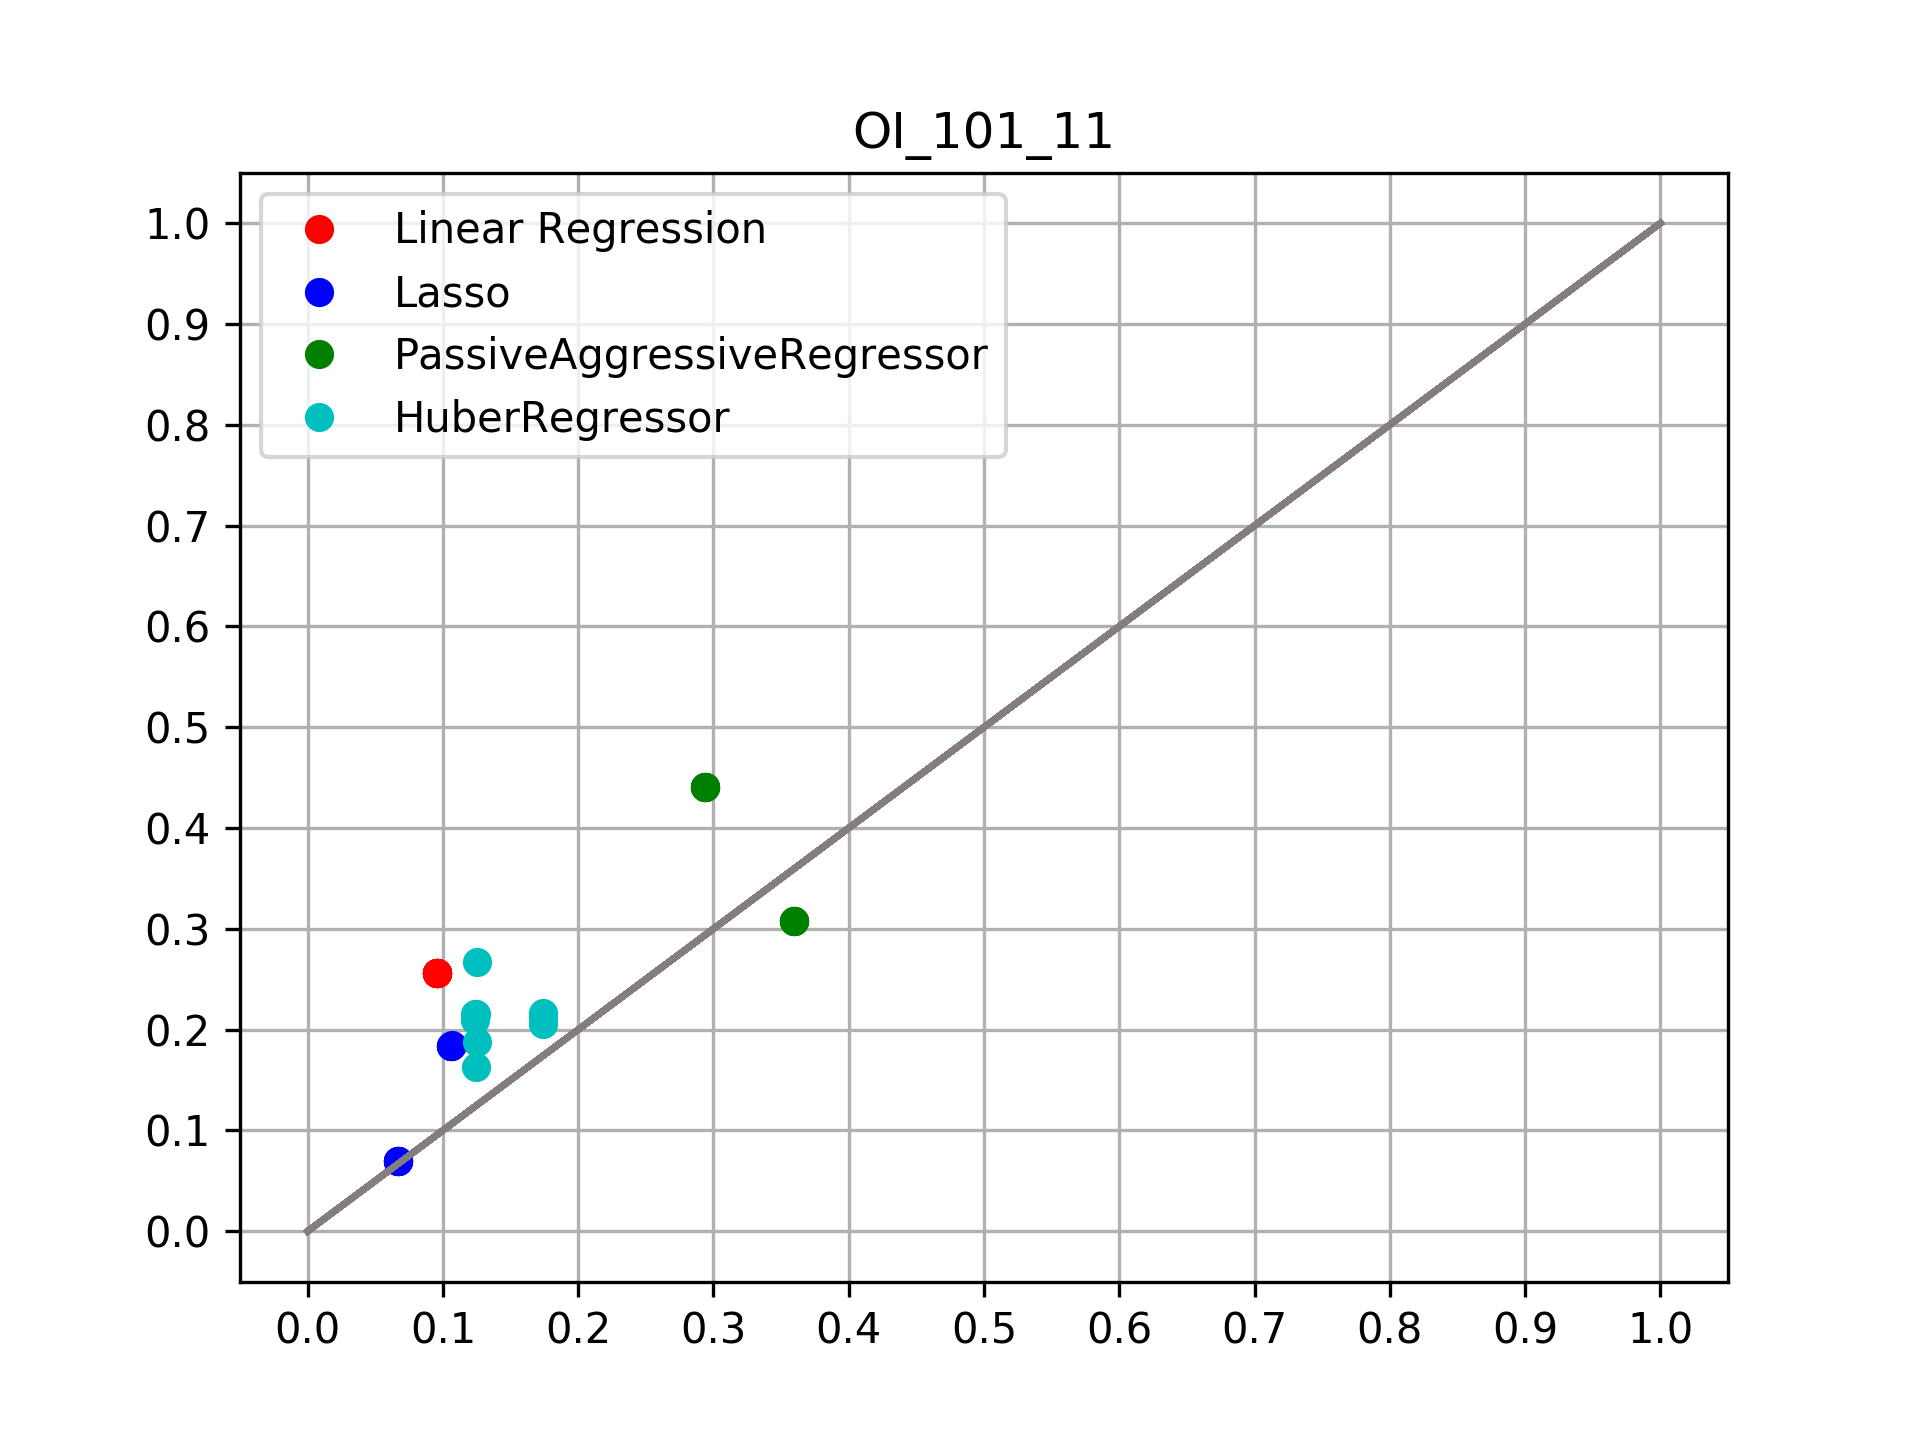
\includegraphics[trim={1cm 0.8cm 1cm 1.37cm},clip,width=0.24\textwidth]
{images/E200_Regression_DCGAN_Adult_16.png}}
\subfigure[Ours,high-privacy,Adult]{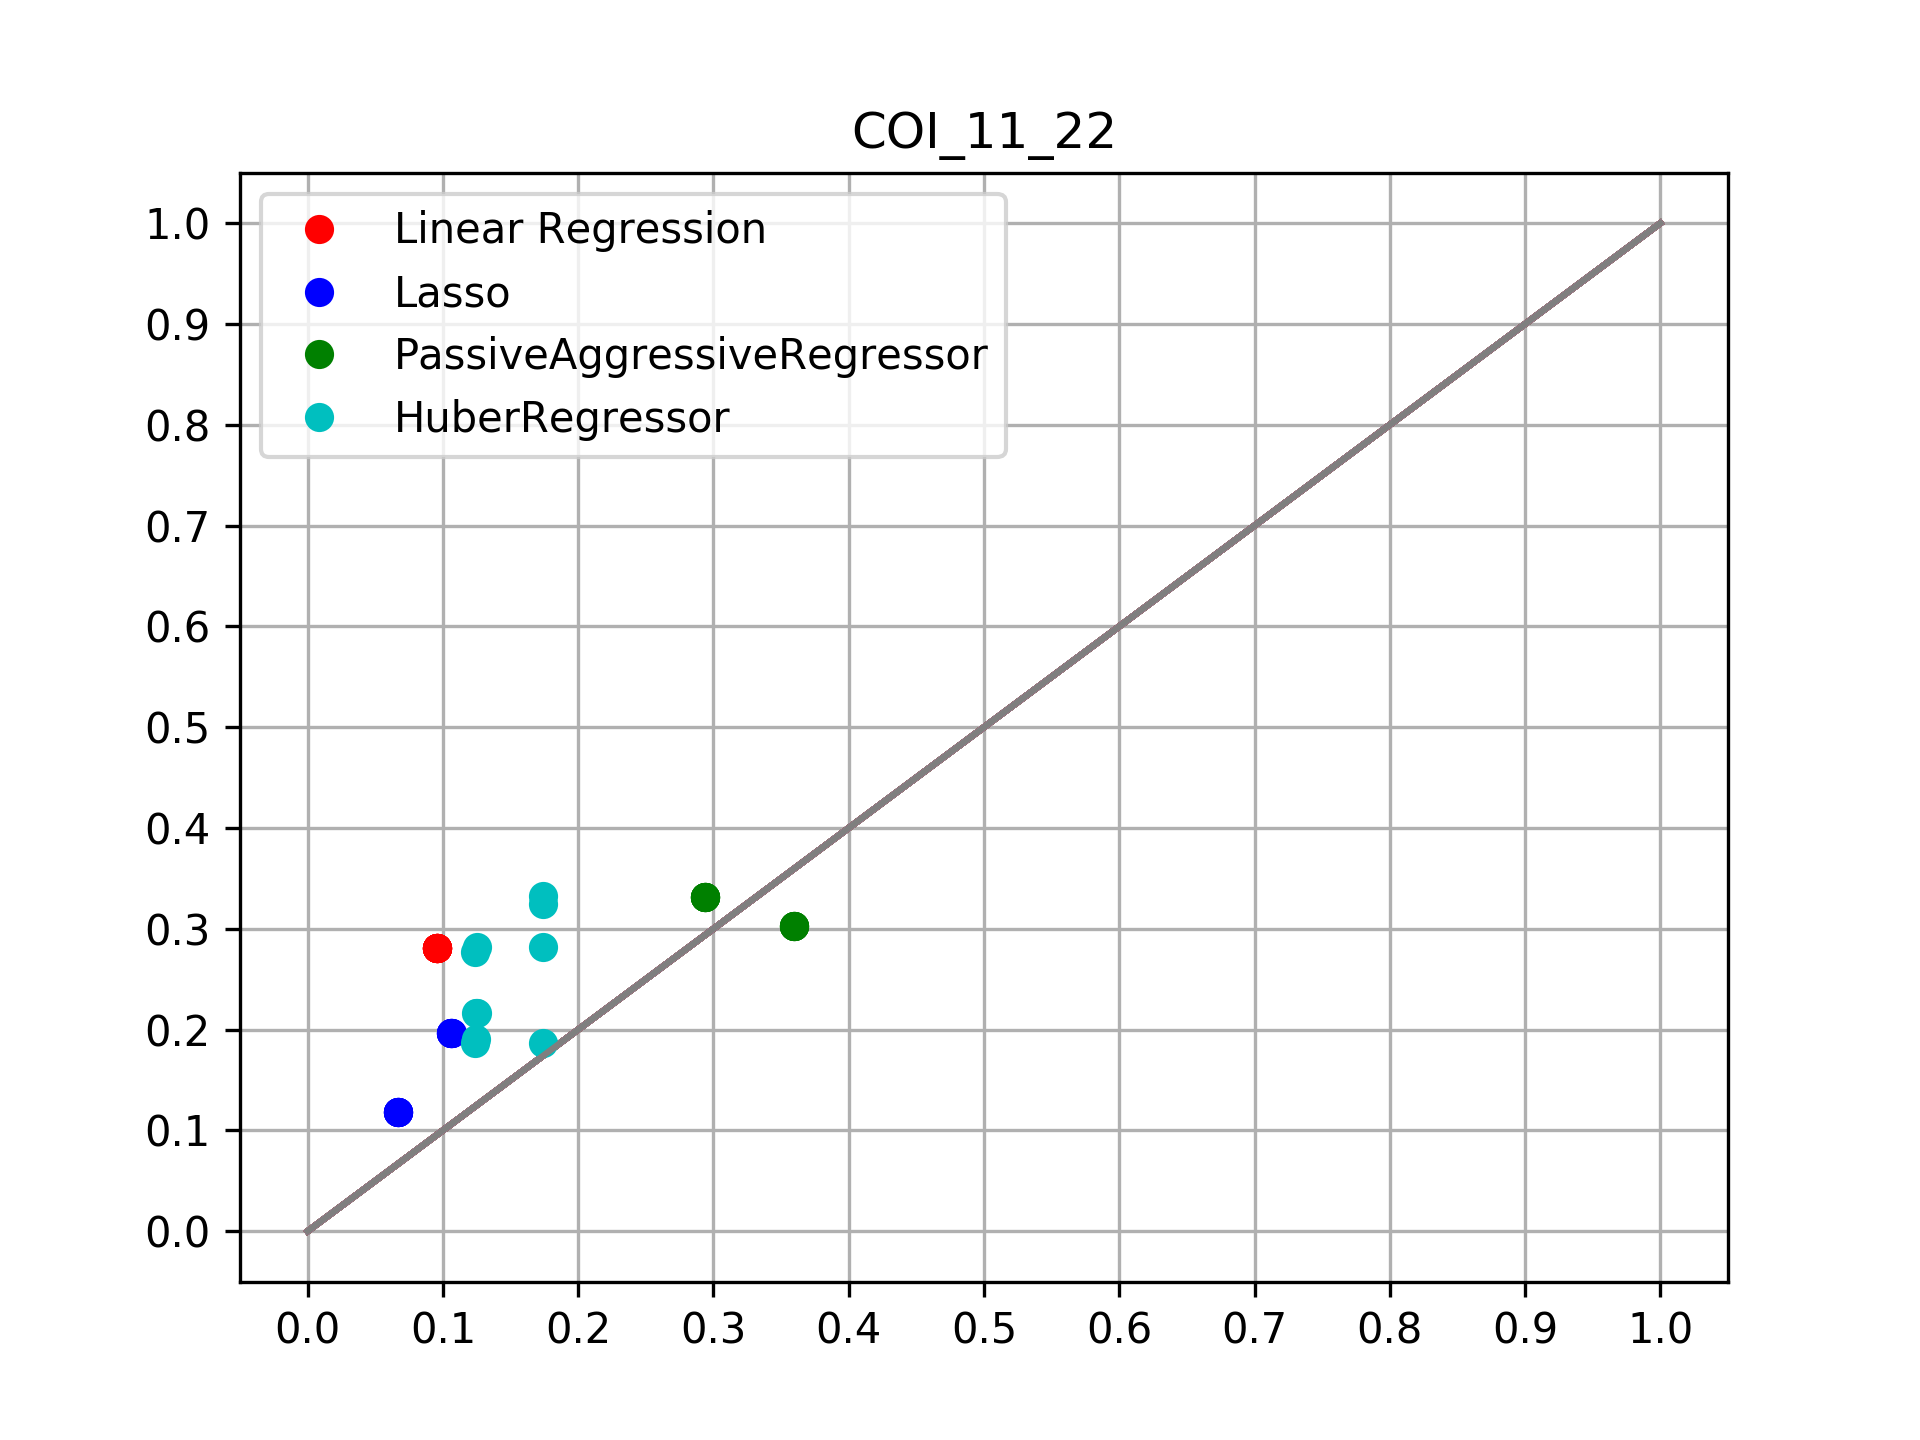
\includegraphics[trim={1cm 0.8cm 1cm 1.37cm},clip,width=0.24\textwidth]
{images/E200_Regression_DCGAN_Adult_4.png}}
\subfigure[The best of ARX,Adult]{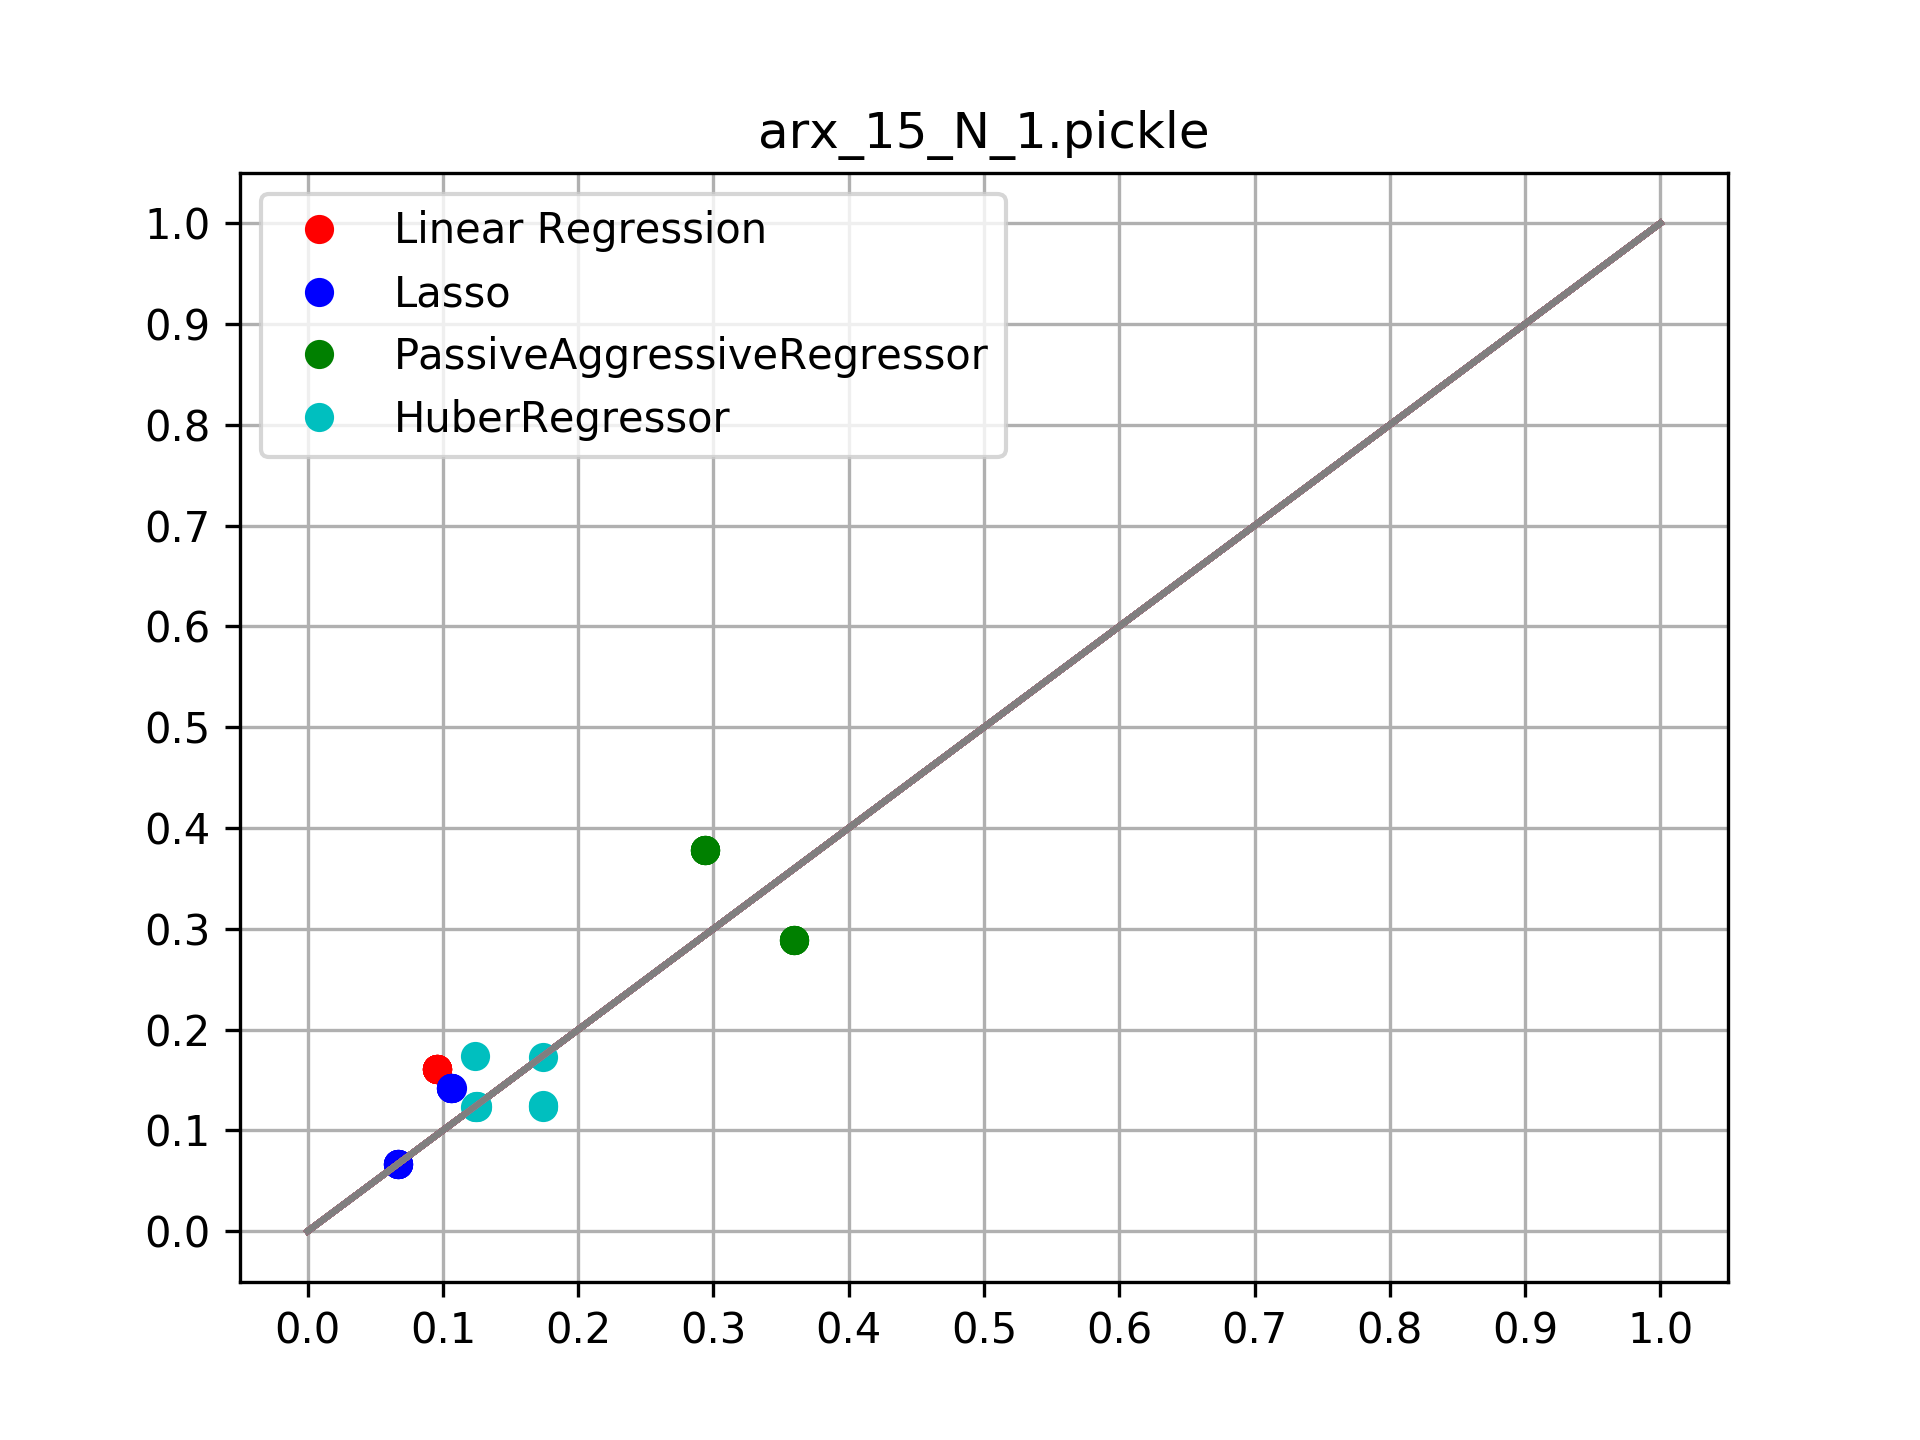
\includegraphics[trim={1cm 0.8cm 1cm 1.37cm},clip,width=0.24\textwidth]
{images/Regression_ARX_Adult_36.png}}
\subfigure[The best of sdcMicro,Adult]{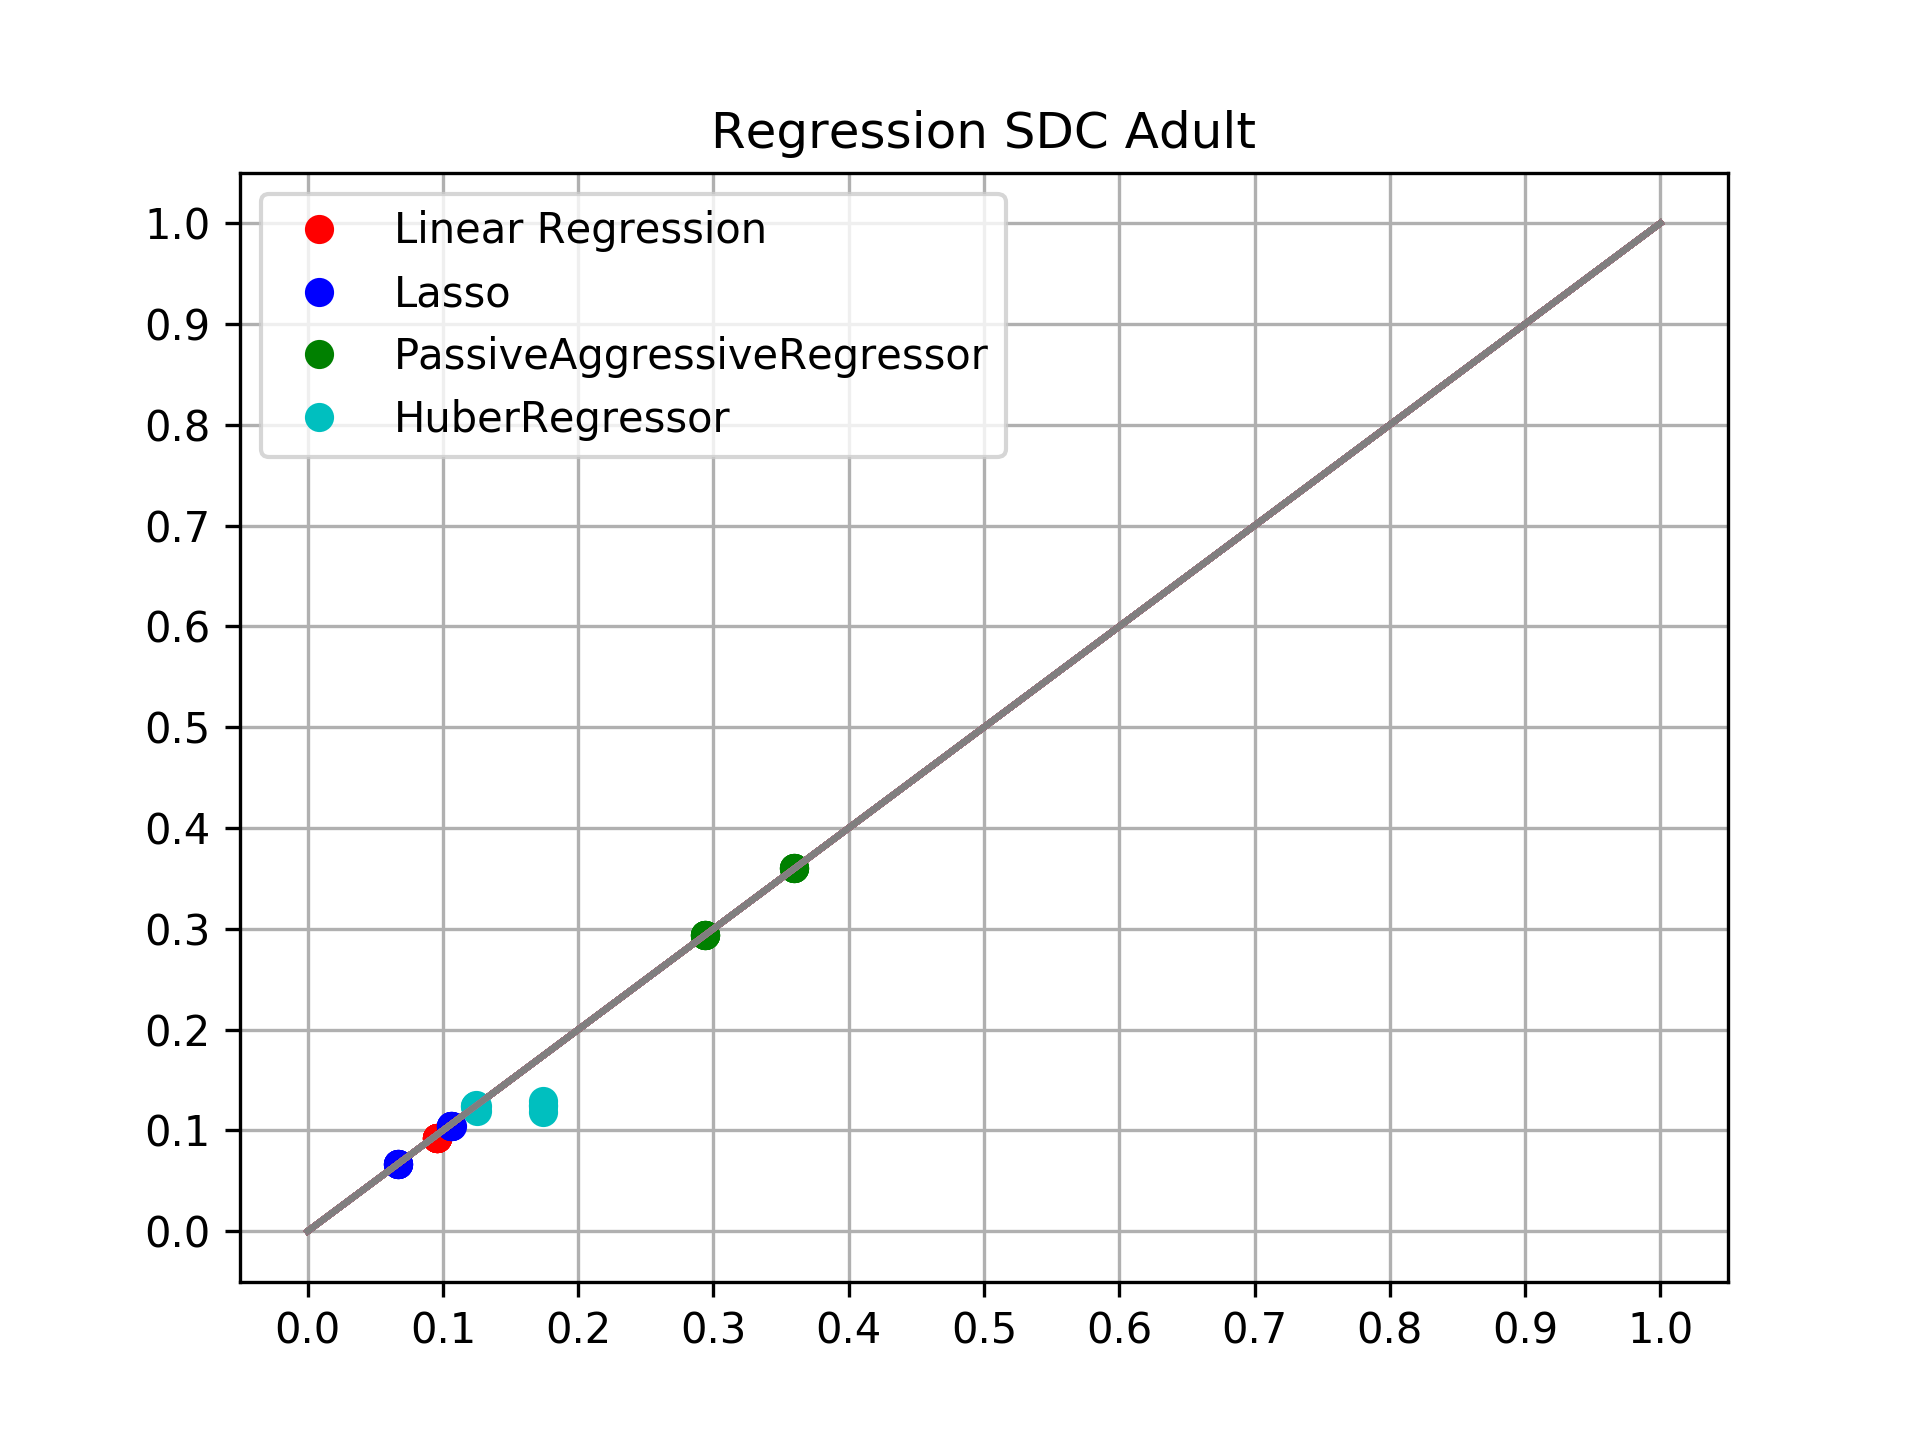
\includegraphics[trim={1cm 0.8cm 1cm 1.37cm},clip,width=0.24\textwidth]
{images/Regression_SDC_Adult.png}}\\
\vspace{-1em}

\subfigure[Ours,low-privacy,Airline]{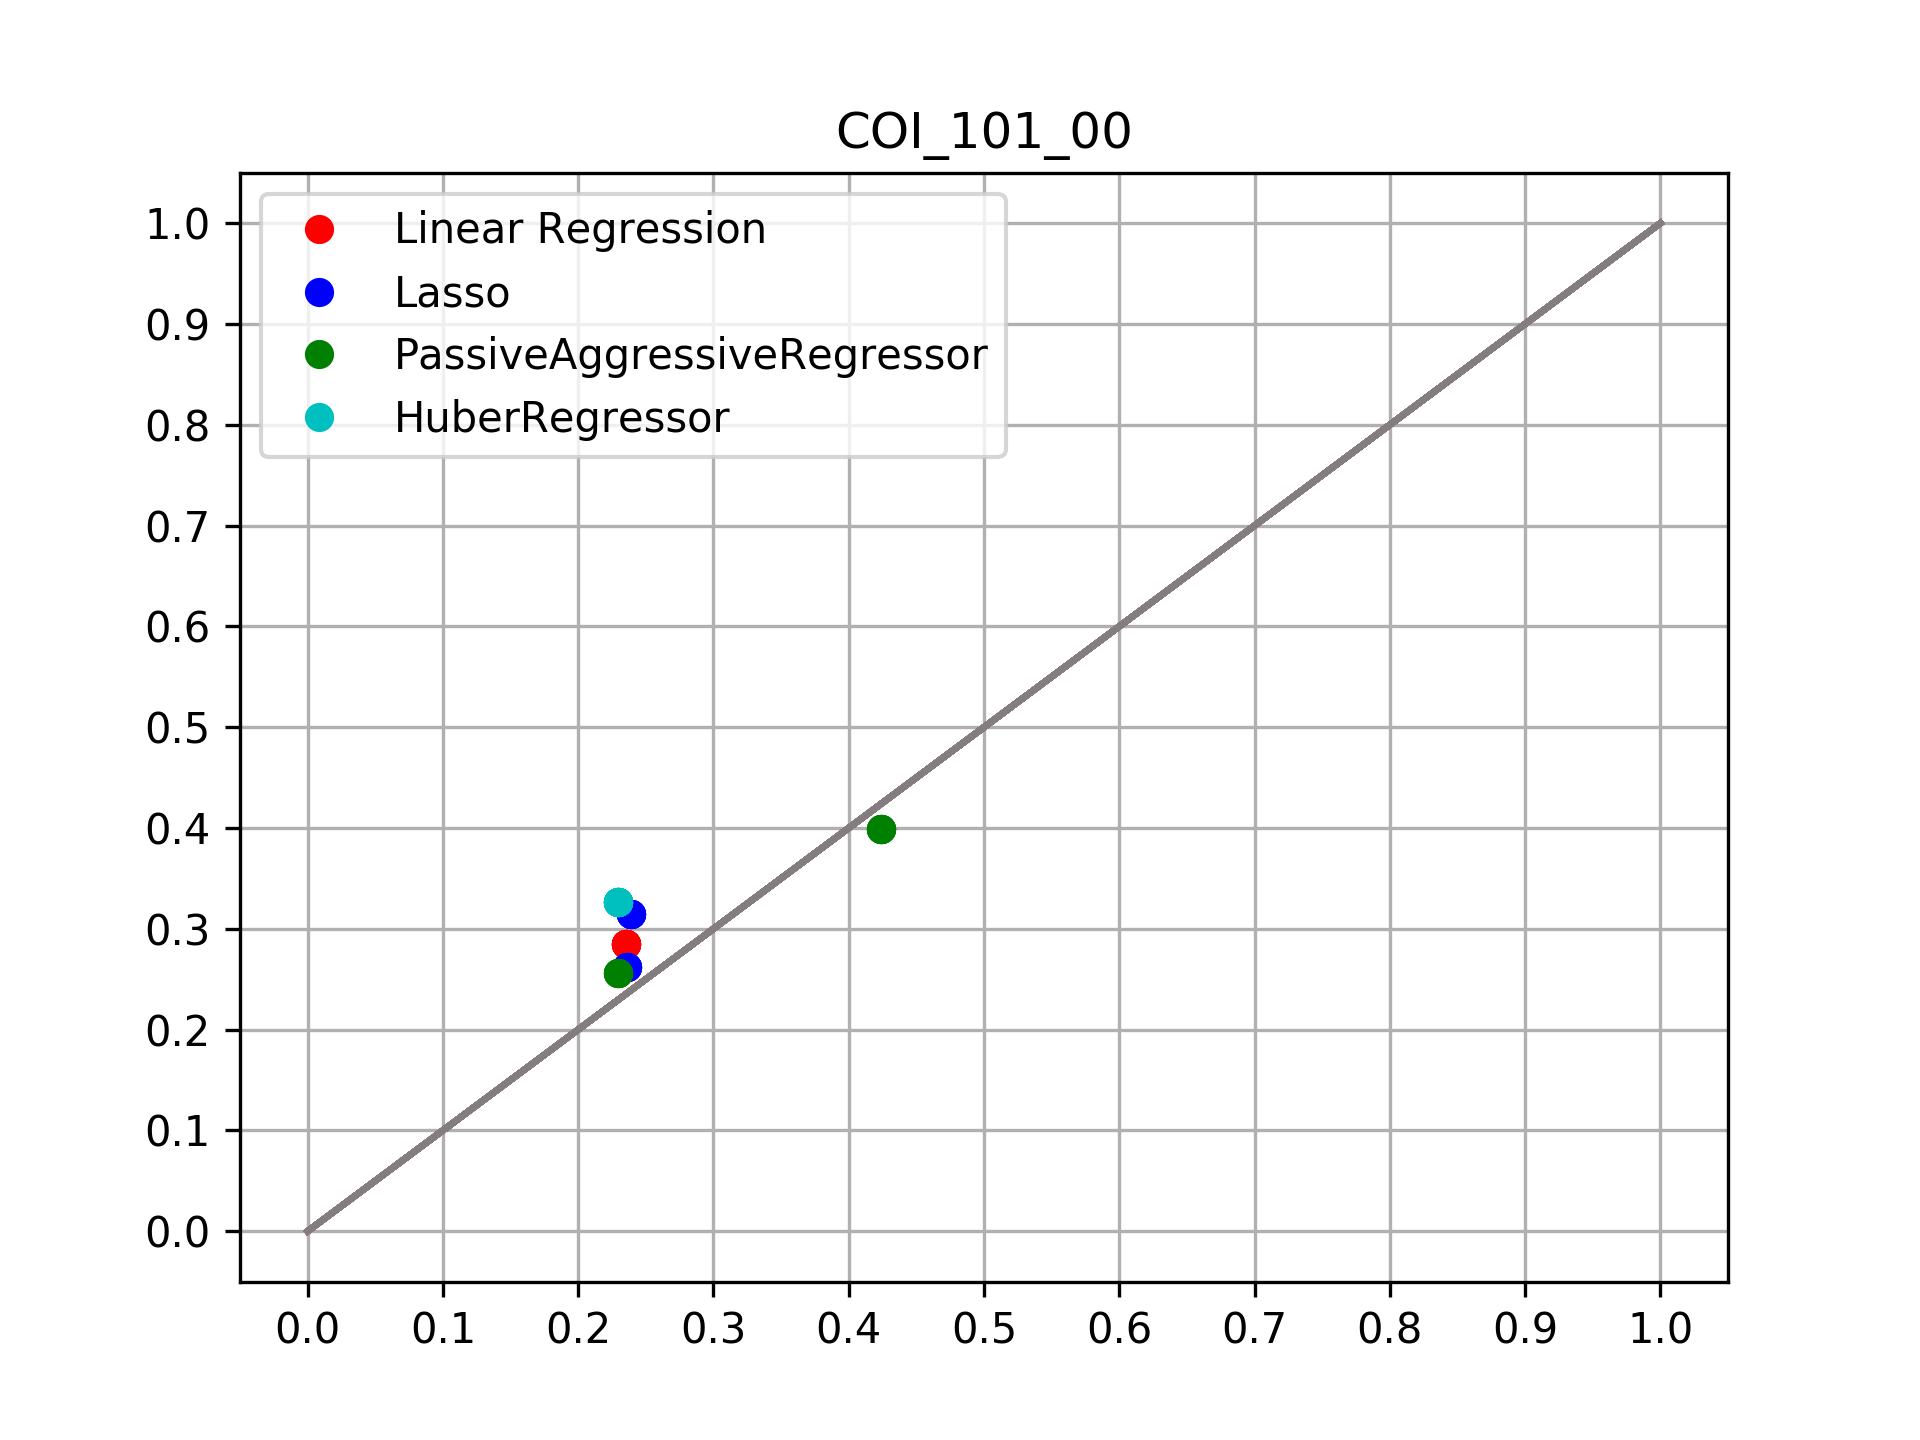
\includegraphics[trim={1cm 0.8cm 1cm 1.37cm},clip,width=0.24\textwidth]
{images/Regression_DCGAN_Ticket_5.png}}
\subfigure[Ours,high-privacy,Airline]{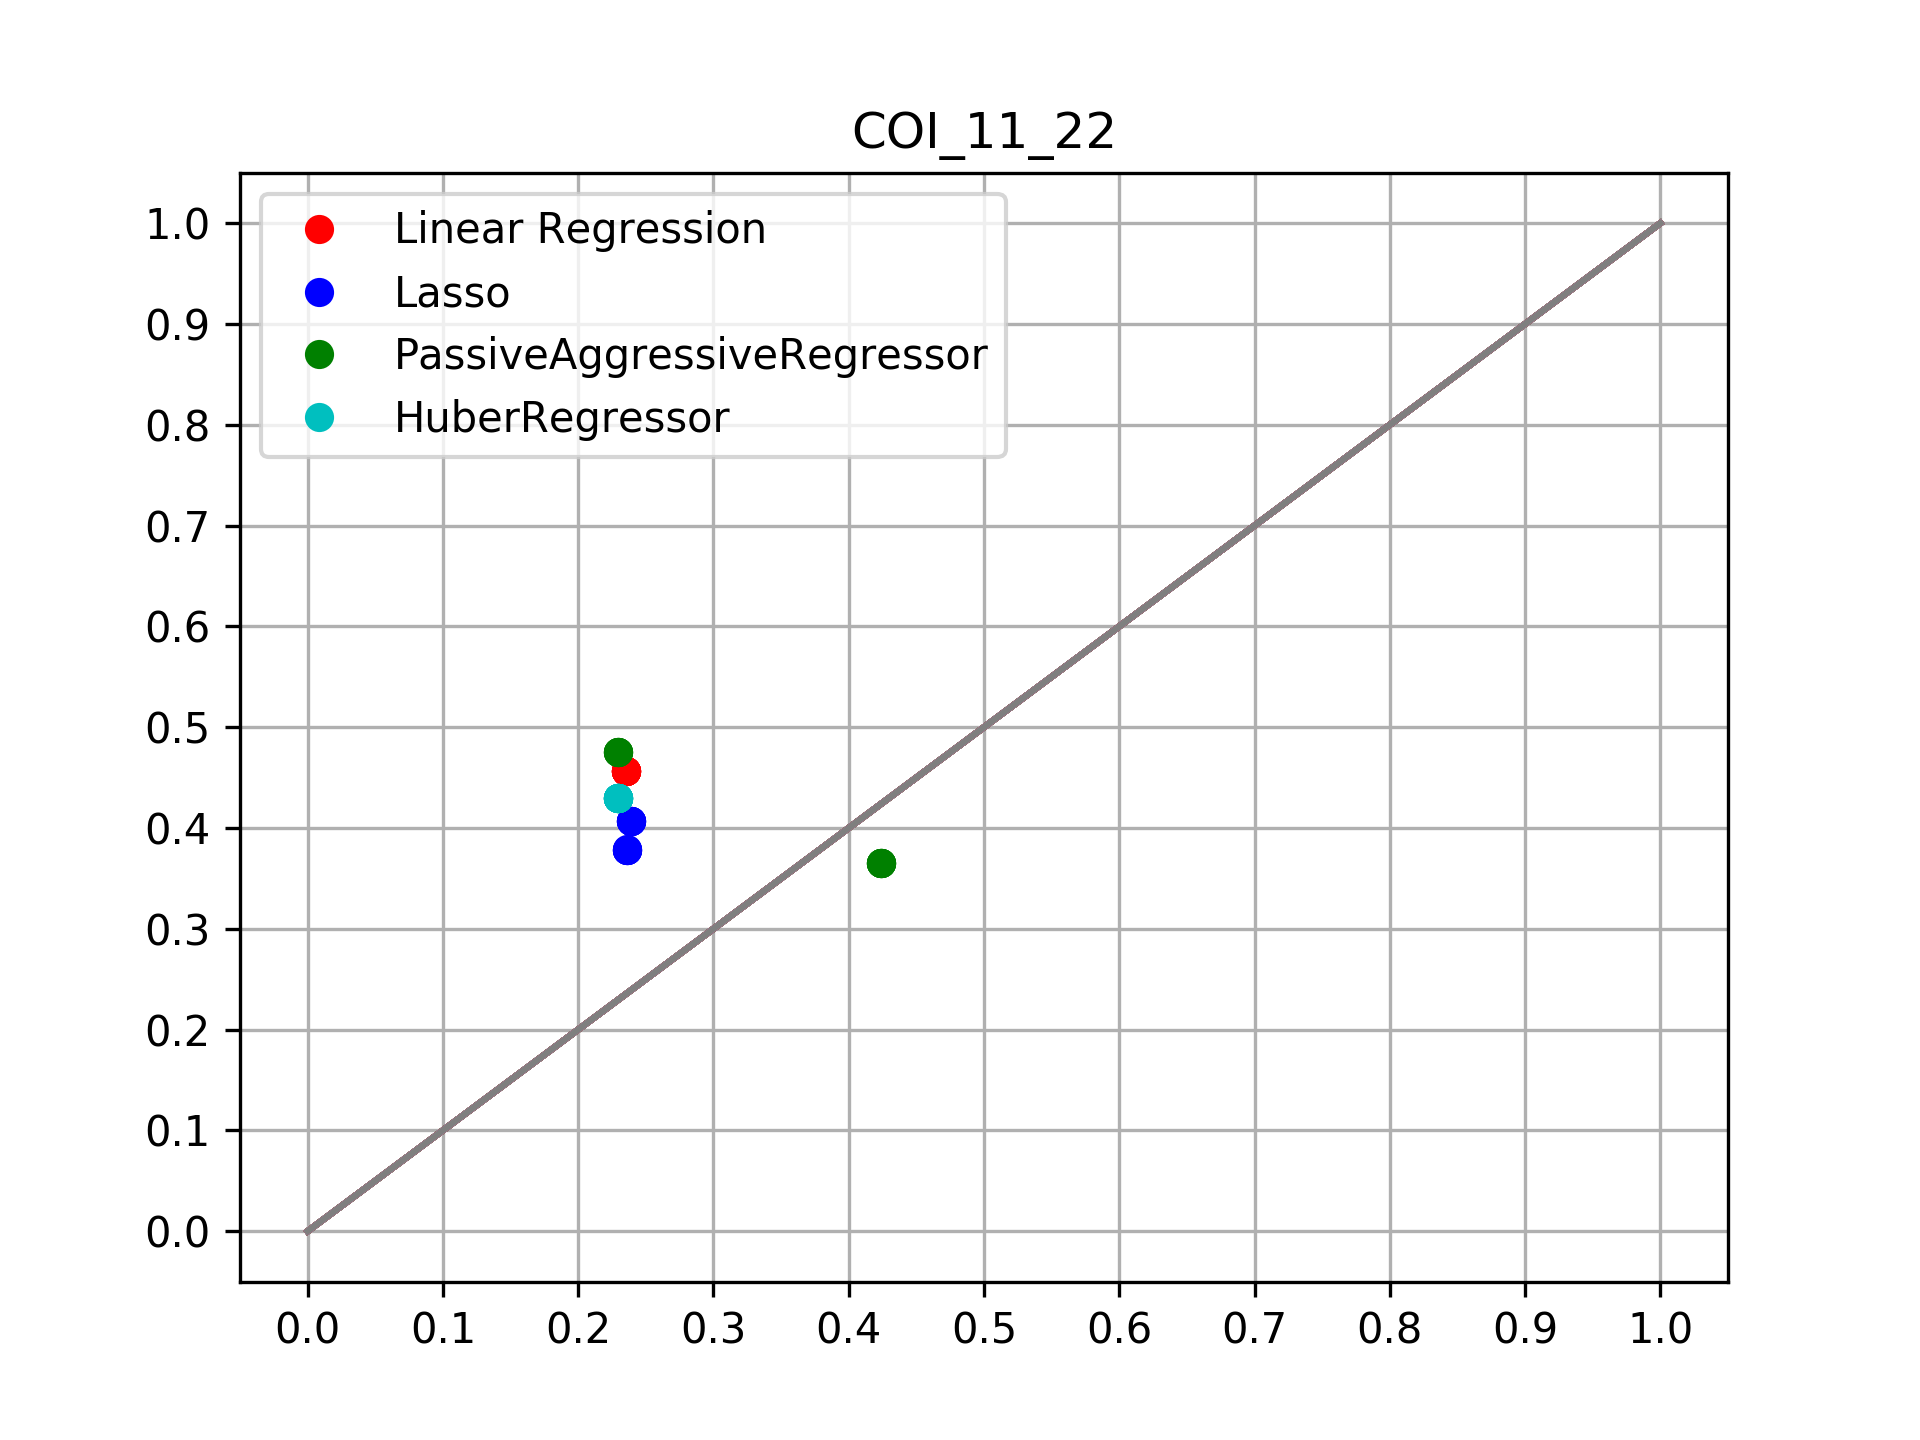
\includegraphics[trim={1cm 0.8cm 1cm 1.37cm},clip,width=0.24\textwidth]
{images/Regression_DCGAN_Ticket_4.png}}
\subfigure[The best of ARX,Airline]{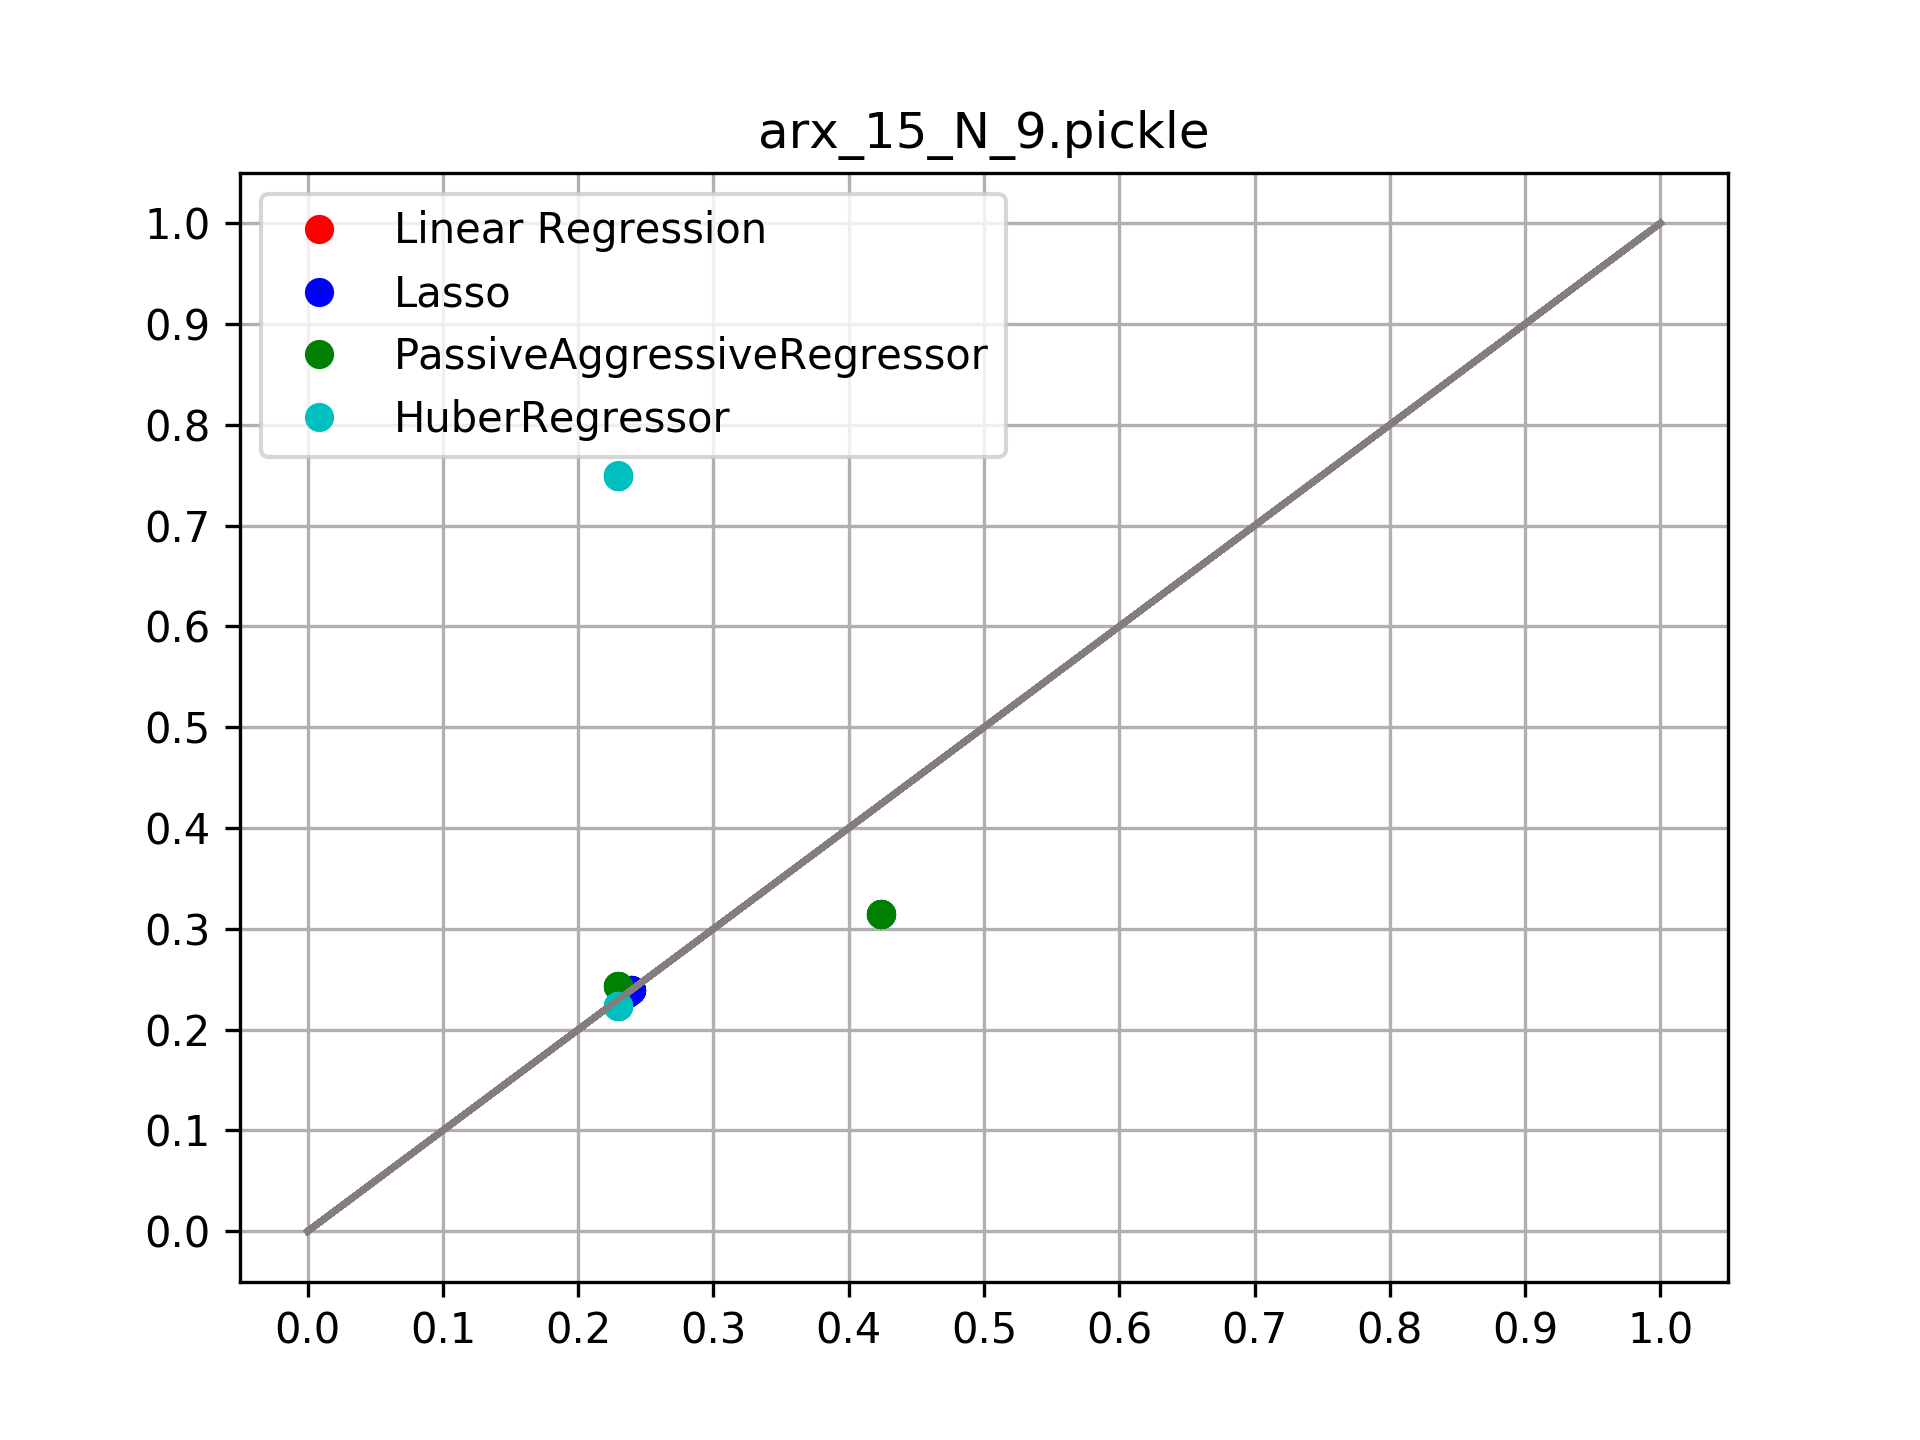
\includegraphics[trim={1cm 0.8cm 1cm 1.37cm},clip,width=0.24\textwidth]
{images/Regression_ARX_Ticket_7.png}}
\subfigure[The best of sdcMicro,Airline]{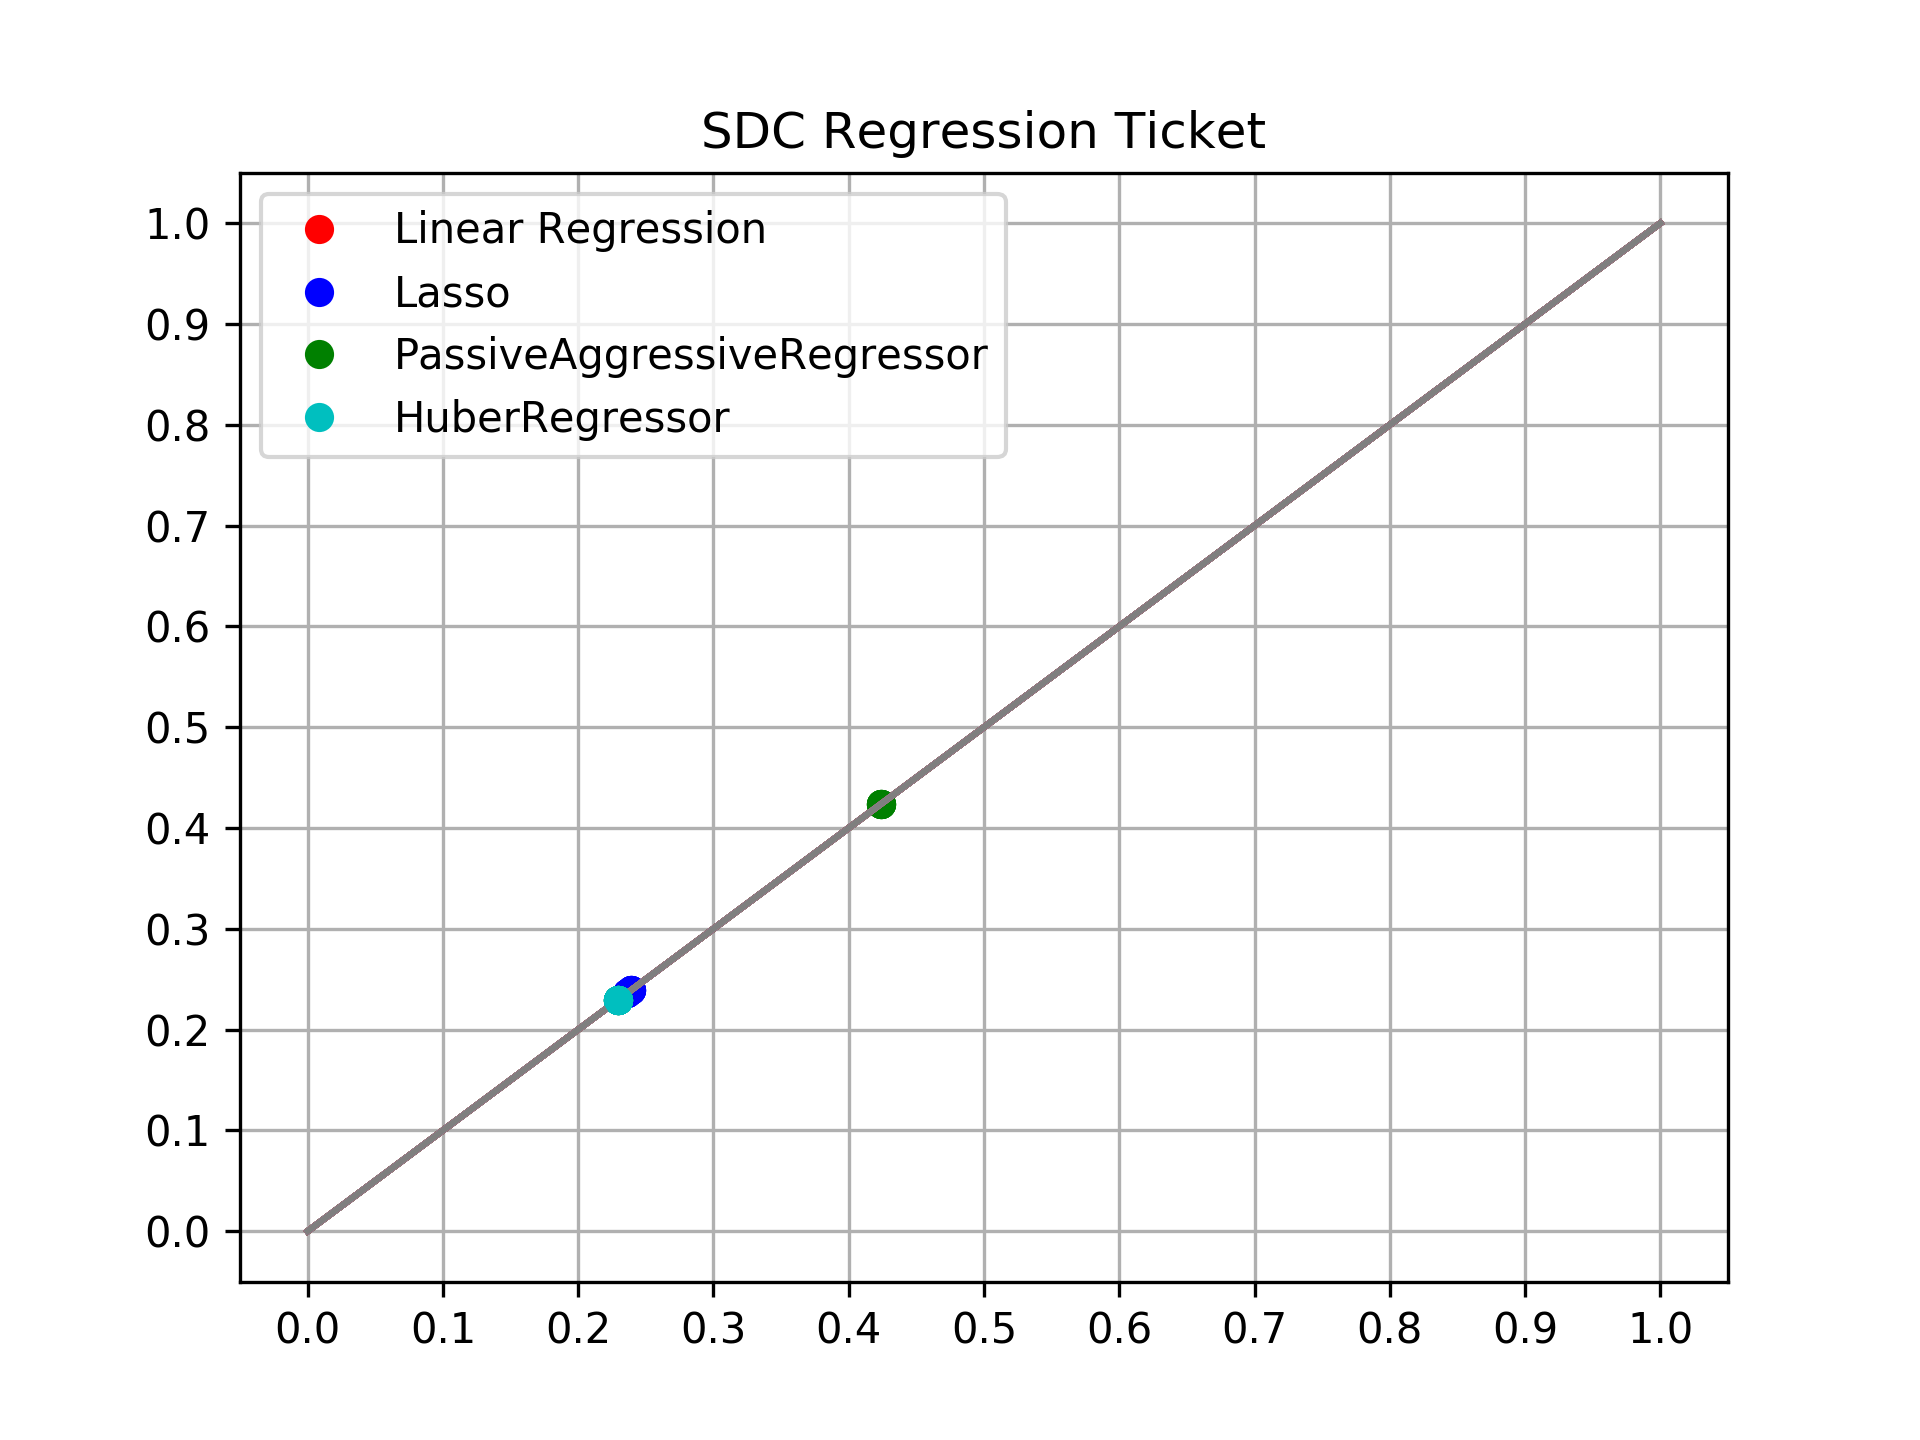
\includegraphics[trim={1cm 0.8cm 1cm 1.37cm},clip,width=0.24\textwidth]
{images/Regression_SDC_Ticket.png}}\\
\vspace{-1em}

\caption{Regression score similarity of ARX, sdcMicro, and table-GAN. We remove DCGAN that did not show reliable performance for space limitations. We plot $(x,y)$ after fixing a regression algorithm and its parameter, where $x$ is the mean relative error (MRE) score of the algorithm trained with the original table and $y$ is the MRE score of the algorithm trained with an anonymized\slash perturbed\slash synthesized table. We test 4 algorithms and 10 parameters for each algorithm. Points on the diagonal line (i.e., $x=y$) mean perfect model compatibility.}\label{fig:rss}
\end{figure*}

\subsubsection{Parameter Setups}
Table-GAN has two parameters $\delta_{mean}$ and $\delta_{sd}$ to control the level of privacy. We consider the following setups: $\delta_{mean}=0$ and $\delta_{sd}=0$ as the \textit{low-privacy setting} and $\delta_{mean}=0.2$ and $\delta_{sd}=0.2$ as the \textit{high-privacy setting}. With the low-privacy setting, realistic records are generated. By increasing the margins, we generate synthetic tables that are dissimilar to the original table.

For $k$-anonymity and $t$-closeness, we tested $k=\{2,5,15\}$ and $t=\{0.01,0.1,0.5, 0.9\}$. For $(\epsilon,d)$-differential privacy and $\delta$-disclosure, we used $\epsilon=\{0.01, 0.5, 1, 2, 5\}$, $d = \{1\mathrm{e}{-6}, 1\mathrm{e}{-3}, 1\mathrm{e}{-1} \}$, and $\delta=\{1, 2\}$. For sdcMicro, we tested the following parameter setups: $pd = \{0.01, 0.5, 1\}$ and $\alpha = \{0.01, 0.5, 1\}$.

For ARX and sdcMicro, we chose the configuration that leads to the best balance between privacy and model compatibility after testing all parameter setups. In the following subsections, we show the results of the best balance cases for ARX and sdcMicro.

\subsection{Distance to the Closest Record}
Let $r$ be a record in the original table. In an anonymized or perturbed table, a record $r'$ that is modified from $r$ always exists. Therefore, their relationship is bijective and weak from re-identification attacks in many cases. In synthetic tables, however, there is no such relationship and thus, we instead find the synthetic record closest to $r$ in Euclidean distance.

Table~\ref{T:dist} shows the average and standard deviation of distances of $(r,c)$ pairs, where $r$ is an original record and $c$ is the record closest to $r$ in an anonymized\slash perturbed\slash synthesized table. It is preferred that the average distance is large and the standard devision is small. A large standard deviation means, even though its average distance is large, there exist some $(r,c)$ pairs that are very close.

As expected, ARX did not change any sensitive values, and its average distance values are always zeros when considering only sensitive attributes. \textbf{Table-GAN with the low-privacy setting shows at most tens of times longer average distance values (and thus, substantially lower success probabilities of re-identification attacks) than ARX and sdcMicro.} Our table-GAN shows very stable average and standard deviation values. Moreover, there is no one-to-one relationship between the original and generated tables. In fact, it is almost impossible to re-identity original values from synthetic values (see our generation examples in Table~\ref{T:org_data} and~\ref{T:syn_data}).
% In general, ARX and sdcMicro show lower distance values than table-GAN in all tested parameter setups.

\subsection{Statistical Comparison}
We show the cumulative distributions and histograms of selected sensitive attributes in Figure~\ref{fig:cd}. We mainly compare DCGAN and the proposed table-GAN after omitting ARX and sdcMicro because they do not significantly change sensitive attributes and show complete matches (i.e., zero-privacy for sensitive attributes) in many cases.

Figures~\ref{fig:cd} (a), (b) and (c) are cumulative distributions of the same attribute in the LACity dataset. Blue lines are by real values in the original table, and orange lines are by synthetic values. Table-GAN with the low-privacy setting produces a more realistic cumulative distribution and a wider range of values than DCGAN and table-GAN with the high-privacy setting. In particular, it is able to reproduce almost all values except for the sparse region emphasized by a red circle in the figure. In fact, this type of neglecting minor cases is one common characteristic of modern machine learning algorithms. They strategically neglect some minor cases to minimize loss functions. However, our model compatibility test shows that this is not critical.

Figures~\ref{fig:cd} (d), (e) and (f) show three cumulative distributions of the same discrete attribute in the Adult dataset by DCGAN and table-GAN. In the low-privacy setting, synthetic values have an almost identical distribution to the original distribution. This pattern is the case in Figures~\ref{fig:cd} (g), (h) and (i) for the Health dataset. In general, table-GAN with the low-privacy setting generates the most similar distributions among all except the anonymization methods.

Histograms are compared in Figures~\ref{fig:cd} (j), (k) and (l). The original distribution has a long-tail distribution, and the low-privacy setting shows an almost perfect match, whereas other methods do not show any similarity. In particular, DCGAN performs very poorly in this test. This result implies the importance of loss functions. Our table-GAN has almost the same neural network architecture as DCGAN. However, we designed considerably more complicated loss definitions. In Figures~\ref{fig:cd} (m), (n) and (o), both of table-GAN and DCGAN successfully reproduce the entire range of values.

To summarize, table-GAN with the low-privacy setting shows very high-quality synthesis performance. In all cases, synthetic tables are statistically similar to the original table. DCGAN performs poorly in many cases because its loss function is not designed for the purpose of table synthesis. Table-GAN with the high-privacy setting performs better than DCGAN.

\subsection{Machine Learning Score Similarity}\label{sec:clas}
We perform several classification and regression tasks to check the model compatibility. These tests are the most important part of our research.  Many anonymization and perturbation methods have been proposed, but their model compatibility is unknown in many cases. We perform in-depth analyses and prove that our table-GAN shows the best balance between privacy level and model compatibility.

\subsubsection{Classification}

In Figure~\ref{fig:ss}, we plot $(x,y)$ pairs, where $x$ is the F-1 score of the model trained with the original table and $y$ is the F-1 score of the model trained with an anonymized\slash perturbed\slash synthesized table in each dataset. We check scores for unknown testing records. Recall that we exclude the grid search, and every $x$ and $y$ pair is calculated using the same machine leaning algorithm with the same parameter setup. We used decision tree, random forest, AdaBoost, and multi-layer perception classifiers and 10 parameter setups for each algorithm (i.e., 40 points in total in a plot). The diagonal line represents perfect model compatibility (i.e., $x=y$ and anonymized\slash perturbed\slash synthetic tables train machine learning algorithms in the same way as the original table). For ARX, we choose the best configuration that shows the best model compatibility in each dataset.

Figures~\ref{fig:ss} (a)-(d) show the F-1 score similarity in the LACity dataset. The tables anonymized by ARX (5-anonymity and 0.01-closeness) and sdcMicro show the best model compatibility in (c) and (d), which is very clear because their modifications to any sensitive attributes are very limited, as shown in the previous DCR tests. ARX with $(\epsilon,d)$-differential privacy and $\delta$-disclouse does not show as good model compatibility as them and we removed it for space limitations. QIDs are also important features in this dataset. Thus, they do not show perfect model compatibility due to the modified QID values\footnote{We applied the label encoding algorithm implemented in scikit-learn (\url{http://scikit-learn.org/stable}) if modified QIDs are not numerical values.}. Table-GAN with the low-privacy setting in (a) shows the second-best model compatibility with very small differences.
% This is a very outstanding result considering the privacy level difference between (a) and (c) in the previous DCR tests. Therefore, our table-GAN has the best balance between privacy perseverance and model compatibility for the LACity dataset.

Figures~\ref{fig:ss} (e)-(h) show the test results from the Adult dataset. Surprisingly, table-GAN with the low-privacy setting in (e) shows model compatibility that is slightly worse than the best ARX\slash sdcMicro cases. In many cases, points by both methods are around the diagonal line. For the Health dataset in Figures~\ref{fig:ss} (i)-(l), our table-GAN shows better model compatibility than all other baseline methods. Only our table-GAN shows practically meaningful model compatibility in this dataset.

Classification scores in the Airline dataset are in Figures~\ref{fig:ss} (m)-(p). ARX and sdcMicro show very good model compatibility. Table-GAN with the low-privacy setting is slightly worse than them. However, its model compatibility is still acceptable.

% All these results prove that the proposed table-GAN's model compatibility is comparable to that of the state-of-the-art methods. \textbf{It is only our table-GAN that shows reasonable model compatibility in all datasets}. ARX and sdcMicro perform poorly in the Health dataset. Moreover, our table-GAN shows consistently higher levels of privacy than other baselines in the previous DCR tests.

\subsubsection{Regression}

In Figure~\ref{fig:rss}, we show the results of the regression model compatibility tests. We follow the same plotting method that shows $(x,y)$ scores. We use mean relative error (MRE) as a base metric to evaluate regression models. Points on the diagonal line means perfect model compatibility. We use the following four regression algorithms and 10 parameter setups for each algorithm: linear regression, Lasso regression, passive aggressive regression, Hurber regression. Because the Health dataset has only binary labels, we could not perform regression tests.

In almost all datasets, table-GAN, ARX and sdcMicro show very good model compatibility. In general, sdcMicro shows better model compatibility than others, which is obvious considering the very low distance in the DCR tests (i.e., low privacy). Our table-GAN shows better model compatibility than ARX.

% Recall that ARX and sdcMicro exhibit poor classification model compatibility in the Health dataset in Figures~\ref{fig:ss} (k) and (l). 




% One interesting result can be observed between table-GAN with the high-privacy setting and DCGAN. Recall that DCGAN performed poorly in previous statistical tests. However, table-GAN with the high-privacy setting has a larger average distance than DCGAN in some cases. This means that our table-GAN is able to provide a high level of privacy while maintaining global statistics better than DCGAN.

% \subsection{Final Remarks and Future Works}
% Existing anonymization methods show good model compatibility (except classification tests in the Health and LACity datasets). However, their privacy level is weak, as shown in the DCR tests.

% Our table-GAN shows very stable model compatibility in all datasets and its privacy level is much higher than other baseline methods.

% We will extend our method to process all data types of relation databases. 
% We performed in-depth analyses in various datasets. In the classification and regression model compatibility tests, we expected at the beginning that existing anonymization methods that do not change sensitive attributes may show the best model compatibility. However, it turns out that it cannot be the case if QIDs are also important features in the classification test (as in the Health dataset). Our table-GAN shows model compatibility comparable to that of existing anonymization methods that do not modify sensitive attributes. Simultaneously, our table-GAN presents at most four times larger values than baseline methods in the DCR tests. This means it provides much higher privacy levels than existing methods.

% \textbf{Our experiments support that the proposed table-GAN exhibits the best trade-off between privacy level and model compatibility among all tested anonymization\slash perturbation\slash generation methods. Even with much larger privacy levels in the DCR tests, it could achieve the best or second best model compatibility in all datasets.} ARX and sdcMicro failed to show reasonable model compatibility in the Health dataset. This further implies the \emph{universality} of our method regardless of input table characteristics.

\begin{table}[t]
\small
\centering
\caption{Sample records in the original LACity table\label{T:org_data}}
\begin{tabular}{|c|c|c|c|c|c|c|}
\hline
        Year  & Salary  & Q1 & Q2 & Q3 & Dept & Job \\ \hline
        2014 & 70386.48  & 16129.89 & 17829.78 & 17678.24 &  98 & 1230 \\
  2013 & 52450.56  & 11331    & 13859.93 & 11968.32 &  70 & 2214\\
  2013 & 89303.76  & 20036.32 & 23479.2  & 21153.6  &  70& 2214\\
  2013 & 60028.96  & 15793.88 & 18560.38 & 16471.18 &  42 & 3184 \\
  2014 & 64553.13  & 14700    & 17313.1  & 15257.17 & 82 & 1368 \\
%   2014 & 65959.92  & 26530.26 & 32978.41 & 25697.5  &  98 & 3181\\
%   2014 & 47911.51  & 13493.87 & 14599.61 & 12619.57 &  4 & 3156\\
%   2013 & 87132.24  & 23355.34 & 23418.8  & 20090.4  &  98 & 1336\\
%   2014 & 55173.05  & 12701.88 & 14797.37 & 12683.46 &  42 & 3141\\
%   2013 & 107821.45 & 23997.87 & 28089.53 & 26816.01 &  70 & 2214\\
\hline
\end{tabular}
% \vspace{1em}
% \centering
% \caption{Sample records in an anonymized table. Dept was anonymized based on the generalization method, and Job was anonymized based on the micro-aggregation method.\label{T:arx_data}}\vspace{-1em}
% \begin{tabular}{|c|c|c|c|c|c|c|}
% \hline

%        Year  & Salary  & Q1 & Q2 & Q3 & Dept & Job \\ \hline
%         2014 & 70386.48  & 16129.89 & 17829.78 & 17678.24 &  4 & 2498 \\
%   2013 & 52450.56  & 11331    & 13859.93 & 11968.32 &  3 & 2214\\
%   2013 & 89303.76  & 20036.32 & 23479.2  & 21153.6  &  3& 2214\\
%   2013 & 60028.96  & 15793.88 & 18560.38 & 16471.18 &  2 & 2112 \\
%   2014 & 64553.13  & 14700    & 17313.1  & 15257.17 & 4 & 2498 \\
%   2014 & 65959.92  & 26530.26 & 32978.41 & 25697.5  &  4 & 2498\\
%   2014 & 47911.51  & 13493.87 & 14599.61 & 12619.57 &  1 & 845\\
%   2013 & 87132.24  & 23355.34 & 23418.8  & 20090.4  &  4 & 2498\\
%   2014 & 55173.05  & 12701.88 & 14797.37 & 12683.46 &  2 & 2112\\
%   2013 & 107821.45 & 23997.87 & 28089.53 & 26816.01 &  3 & 2214\\
% \hline
% \end{tabular}
\centering
\caption{Sample records in the synthesized table by table-GAN with the low-privacy setting. For each real record in Table~\ref{T:org_data}, we have chosen the closest synthetic record in Euclidean distance.\label{T:syn_data}}
\begin{tabular}{|c|c|c|c|c|c|c|}
\hline
       Year  & Salary  & Q1 & Q2 & Q3 & Dept & Job \\ \hline 
2013& 72005.93  & 11747.34 & 17186.00 & 19557.64 & 50 & 1451 \\
2013 & 59747.90  & 4369.88  & 13377.60 & 22311.95 & 73 & 1248 \\
2013 & 85600.46  & 17993.01 & 25420.13 & 27127.87 & 46 & 2025 \\
2013 & 65156.87  & 11011.99 & 20201.47 & 23563.72 & 67 & 1887 \\
2014 & 68638.75  & 9642.26  & 13674.69 & 15680.99 & 51 & 998  \\
% 2014 & 73140.91  & 14474.15 & 28872.33 & 30307.91 & 71 & 2279 \\
% 2013 & 59747.90  & 4369.88  & 13377.60 & 22311.95 & 73 & 1248 \\
% 2013 & 83500.37  & 18666.59 & 24082.54 & 26570.42 & 41 & 1868 \\
% 2013 & 67157.95  & 8104.19  & 13731.41 & 16964.88 & 53 & 1076 \\
% 2013 & 91477.97  & 19280.95 & 33788.71 & 36766.97 & 52 & 2474\\
\hline
\end{tabular}
% \centering
% \caption{Records in a synthesized (fake) Table-Sensitive +QID}
% \label{T:syn_data}
% \begin{tabular}{|c|c|c|c|c|c|c|}
% \hline
%        Year  & Salary  & Q1 & Q2 & Q3 & Dept & Job \\ \hline 
% 2013 & 72005.93  & 11747.34 & 17186.00 & 19557.64 & 50 & 1451 \\
% 2013 & 59747.90  & 4369.88  & 13377.60 & 22311.95 & 73 & 1248 \\
% 2013 & 85600.46  & 17993.01 & 25420.13 & 27127.87 & 46 & 2025 \\
% 2013 & 65156.87  & 11011.99 & 20201.47 & 23563.72 & 67 & 1888 \\
% 2014 & 68638.75  & 9642.26  & 13674.69 & 15680.99 & 51 & 998  \\
% 2014 & 73140.91  & 14474.15 & 28872.33 & 30307.91 & 71 & 2279 \\
% 2013 & 59747.90  & 4369.88  & 13377.60 & 22311.95 & 73 & 1248 \\
% 2013 & 83500.37  & 18666.59 & 24082.54 & 26570.42 & 41 & 1868 \\
% 2013 & 67157.95  & 8104.19  & 13731.41 & 16964.88 & 53 & 1077 \\
% 2013 & 91477.97  & 19280.95 & 33788.71 & 36766.97 & 53 & 2475\\
% \hline
% \end{tabular}
\end{table}

\subsection{Generation Example}
We show generation examples based on the LACity dataset in Table~\ref{T:syn_data}. Sample records of the original LACity table are shown in Table~\ref{T:org_data} after selecting a subset of columns for space reasons.

% Table~\ref{T:arx_data} is generated by ARX based on $k$-anonymity and $t$-closeness. The Dept attribute of the table is anonymized using the generalization method that changes values to ranges. After applying label encoding, we could obtain numbers. The Job attribute is anonymized with the micro-aggregation technique that converts values into the most frequent value of equivalence classes, called \textit{mode}. As expected, sensitive attributes are disclosed without any modifications. Consequently, we expected perfect compatibility with the anonymized table. However, its model compatibility is considerably worse than our expectation in Figures~\ref{fig:ss} (c) because QIDs are also key attributes to predict the ground-truth label of the LACity dataset.

Our table-GAN (with the low-privacy setting) generates Table~\ref{T:syn_data}. Because there is no one-to-one correspondence between Table~\ref{T:org_data} and Table~\ref{T:syn_data}, we select a synthetic record closest to each real record of Table~\ref{T:org_data} after attribute-wise normalization. As shown, real records have very different values from the closest synthetic record. It is almost impossible to identify original records in the synthetic table. \textbf{Surprisingly, its model compatibility is comparable to other anonymized tables (where sensitive values are not modified) and in some other datasets, our table-GAN shows better model compatibility than other baseline methods. This is a remarkable result because we achieve a practically meaningful level of model compatibility without disclosing any real records}.